%!TEX root=main.tex
\chapter{数据中心与可编程网卡概论}
\label{chapter:background}

本章介绍全文的背景和相关工作。第 1 节回顾数据中心的发展历史,展望数据中心的未来趋势,提出数据中心的性能开销与挑战,以及性能优化的可能方向。第 2 节综述数据中心计算、内存、存储和网络互连系统硬件的发展趋势。第 3 节讨论基于专用芯片、网络处理器、通用处理器、FPGA 的四种可编程网卡架构。第 4 节调研可编程网卡在微软 Azure、亚马逊 AWS 等数据中心的部署。

\section{数据中心全栈优化的历史机遇}
\label{background:sec:challenge}

\subsection{数据中心的细粒度计算趋势}
\label{background:sec:datacenter-granular}


从 20 世纪 50 年代计算机的诞生到 90 年代互联网兴起前,人类的算力大部分用于高性能计算、数字化企业和个人计算机(PC),其产生的数据大多存储在一个个信息孤岛上。需要处理大量信息的大型机乃至超级计算机一般采用软硬件一体化系统,即软硬件是由同一个公司团队开发的。由于采用了高速硬件互连、硬件冗余,这些系统往往同时具备高性能和高可靠性,但成本随系统规模的扩大急剧增加。为了充分利用昂贵的计算机,虚拟化的概念应运而生。其中 20 世纪 50 至 60 年代的分时系统 \cite{strachey1959time,amdahl1964architecture} 实现了多个用户任务分时复用硬件,发展成为 70 年代 UNIX 等现代操作系统 \cite{bach1986design} 的前身。20 世纪 70 至 90 年代,虚拟机监视器(Virtual Machine Monitor,VMM)进一步实现了多个操作系统分时复用硬件 \cite{popek1974formal,agesen2010evolution},为云计算的发展做了技术准备。

在现代史上,产品传输成本较低、能够赋能各行各业的通用目的技术(General Purpose Technology,GPT)大多发展成为按需租用的社会基础服务。
一个典型的例子是电力。电力作为工业和城市的基础资源,早期也是由需要电的工厂、学校等自己购买发电机来发电,逐渐才形成今天庞大而复杂的电力系统,由发电、输电、变电、配售电等多个标准化的环节构成,客户只需要按需租用电力资源。
计算机作为信息社会的基础设施,自然也不例外。从早期的客户自己购买和运维计算机、操作系统、应用程序,到今天被称为云计算的按需租用计算、存储和网络资源甚至更上层的应用服务。
未来,对提供互联网服务的公司和个人而言,自建数据中心、购买和运维服务器就像自建发电厂、购买和维护发电机一样,在大多数场景下成本很高且没有必要。

21 世纪的第一个十年,互联网的发展让越来越多的企业需要提供 24 小时运行的网络服务,互联网数据中心(Internet Data Center,IDC)托管服务逐渐兴起。然而,IDC 托管需要客户事先购买服务器硬件,并需要运维人员维护,有较高的资产成本(capex)和运营成本(opex)。很多企业的网络服务一方面具有较高的季节性(如亚马逊的黑五促销),因此在闲时大量的计算资源被闲置;另一方面数据和用户规模的扩张很快,给购买硬件和 IDC 选址带来了时间压力。为此,虚拟机托管服务提供了按需租用的虚拟机资源,实现了服务器资源按 CPU 核的切片和在不同客户间的分时复用,也便于客户内部运维人员的管理和调度。

云计算是虚拟机托管服务的升级版,标志性的变革是计算和存储的解耦。虚拟主机托管服务把一台主机上的计算和存储资源分片成多个虚拟机,一旦主机的硬件或虚拟化软件(hypervisor)发生故障,虚拟机也就停机,其中的数据还有丢失的风险。在云计算中,虚拟机的存储资源在分布式存储系统中有多个副本,从而计算节点发生故障时可以从其他计算节点重启虚拟机,存储节点的故障则一般对客户透明。计算和存储的解耦不仅大大提高了服务可用性和数据安全性,也方便了虚拟化软件升级和虚拟机热迁移。

除了与其他公司共享硬件资源,IT 企业使用云计算进行虚拟化还有一个目的,即复用硬件基础设施,为公司内不同类型的服务提供不同的服务质量保证。例如,5G 核心网需要在同一张物理网络上支持多种不同需求的服务,如 5G 的三种典型应用场景:极高带宽(eMBB)、极大规模(MTC)、极低和极稳定延迟(URLLC)。高带宽、大规模、低延迟等需求某种程度上是互相矛盾的,需要根据应用的需求进行权衡。因此,3GPP 标准中指明了 5G 核心网采用基于服务的系统架构,这些服务需要使用虚拟化的网络功能来实现 \cite{3gpp-23501,3gpp-38300}。

云计算并不止步于基于虚拟机的虚拟化。计算的粒度还在不断降低。2013 年 Docker 框架提出以来,大量互联网公司使用容器(container)部署服务 \cite{bernstein2014containers}。容器不仅是轻量级的虚拟机,更重要的是重新定义了互联网服务的架构,从少量复杂的宏服务(macroservice)解耦合成大量简单的微服务(microservice)。每个微服务使用容器的形式部署,可以实现高效的可扩放数据中心调度、软件依赖管理和微服务间的隔离,提高开发、测试和运维的效率。微服务架构相比传统架构的计算粒度更细,因而对总请求服务能力的需求更高,对微服务间通信的需求也很高。
例如,微信有超过 3000 个微服务运行在超过 2 万台服务器上。入口层的微服务每天响应 100 亿至 1000 亿次用户请求,而每个用户请求会在系统内部触发更多的微服务请求,因此整个微信后端每秒需要响应数以亿计的微服务请求 \cite{zhou2018overload}。

基于容器的微服务并不是计算粒度缩小的终点。容器内仍然运行着传统操作系统的进程,这些进程即使没有外部请求,也在消耗一定的内存资源。为了保证容器能及时响应用户随时可能到来的请求,CPU 等计算资源也需要预留。容器也需要占据一定的存储空间。因此,云服务商需要为每个容器预留计算、内存和存储资源,并为这些预留的资源收费。容器的扩放、调度和运维也需要容器的使用者(即网络服务开发者)负责,虽然有 Kubernetes \cite{burns2016borg} 等开源框架,但也增加了容器使用者的负担。2015 年,亚马逊 AWS 推出了名为 Lambda 的无服务器计算(serverless computing)服务,使得用户只需在云服务商的编程框架内编写事件驱动的业务代码,而把执行环境、扩放、调度等任务都留给云服务商。目前,亚马逊、微软、谷歌、阿里、腾讯等主流云服务商都提供了无服务器计算服务。

从物理机到虚拟机,再到基于容器的微服务,以及未来的函数计算,数据中心的计算粒度正在变得越来越细。下文将讨论细粒度计算对资源虚拟化和通信的需求对数据中心系统的挑战。

\subsection{数据中心的分布式计算趋势}
\label{background:sec:datacenter-distributed}

除了细粒度计算,数据中心的另一大趋势是分布式计算。

20 世纪末,连接信息孤岛的搜索引擎拉开了互联网时代的序幕。数据中心不仅需要搜集、处理和索引海量信息,还需要实时响应大量用户的信息检索请求。传统的超级计算机、大型机和企业级存储不仅成本高昂,也无法满足海量信息存储和用户请求处理的可扩放性。为此,Google 提出用普通商用服务器组建可扩放的数据中心,用软件来实现存储的分区和冗余、用户请求的分派,在相对不可靠的硬件基础上组建起容错的系统 \cite{dean2008mapreduce}。

这些普通商用服务器之所以成本较低,是因为它的架构与大量商用的个人计算机(PC)类似,CPU、内存、主板、硬盘、网卡等组成部分都是标准组件,由各个专业公司独立设计实现。操作系统、数据库、Web 服务器等软件也是标准化的,或者由专业公司开发,或者是开源软件。产量大的标准组件能更好地平摊研发、流片等一次性工程费用(Non-Recurring Engineering,NRE),从而降低标准组件的价格。由标准组件构成的系统虽然降低了数据中心的软硬件成本,但也给标准组件的开发者施加了限制:大家需要遵守标准组件之间的接口和协议,只能在自己的边界内创新。数据中心系统的搭建者则只能像搭积木一样组合标准组件,而很难通盘考虑、全局优化。

自 21 世纪的第一个十年,互联网公司的数据规模迅速膨胀,以 Hadoop \cite{white2012hadoop}、Spark \cite{zaharia2010spark} 为代表的大规模数据处理开始兴起。相比信息检索、Web 信息服务等相对容易并行化的工作负载,大规模数据处理是不容易并行处理并获得线性加速的。
自 2012 年起,神经网络开始复兴,深度学习成为机器学习的新范式,也使人工智能进入了持续至今的又一次高潮。在大规模机器学习训练中,每一个阶段需要各个节点之间同步模型,因而对通信性能提出了很高的要求 \cite{distributed-ml}。
大规模数据处理与机器学习对分布式系统带来了很多挑战。频繁的进程(或计算节点,下统称为进程)间通信对数据中心网络的延迟和吞吐量都提出了很高的要求,这也推动了数据中心网络近十年来从 1 Gbps 到 40 至 100 Gbps 的性能飞跃。有了高性能的网络硬件并不意味着分布式系统通信性能的提高。事实上,传统操作系统的 ``数据中心税'' 使分布式应用难以充分利用数据中心网络硬件的高性能。因此,需要从系统的层面上优化分布式系统中的进程间通信原语,使其与硬件性能相匹配。

分布式系统中的进程间通信有消息传递和共享内存两种范式 \cite{kshemkalyani2011distributed}。在消息传递范式中,进程把需要发送的数据结构序列化成一个字符串,通过网络消息发送给另一个进程。在共享内存范式中,多个进程共享内存空间,一个进程写入的内容能被所有进程读取。在很多情况下,共享内存的抽象层次太低,多个进程同时写入时的进程间同步开销很高,因此共享数据结构成为更多分布式应用的选择。键-值(key-value)映射是一种常用基本数据结构,也可以组成更复杂的数据结构,因此共享键-值存储(key-value storage)是分布式系统中取代共享内存的常用共享数据结构存储。消息传递和共享数据结构两种进程间通信范式在不同的场景下各有优劣,它们对分布式系统的性能都很重要。本文第 \ref{chapter:clicknp} 章和第 \ref{chapter:socksdirect} 章致力于提升消息传递的性能。本文第 \ref{chapter:kvdirect} 章将以键-值存储作为典型例子,致力于提高共享数据结构存储的性能。

2019 年,加州大学伯克利分校对无服务器计算的预测报告 \cite{jonas2019cloud} 表明,尽管无服务器计算的范式有诸多优势,也是各大云服务商争相推广的新服务,但由于云存储的性能问题和临时存储服务的缺失,很多类型的应用使用无服务器计算的性能和成本不理想。
事实上,目前的大数据处理框架(如 Spark \cite{zaharia2010spark})、分布式强化学习框架(如 Ray \cite{moritz2018ray})、云计算厂商的数据湖(data lake)服务 \cite{ramakrishnan2017azure} 中,为了容错性和可扩放性,数据处理函数一般是无状态的,已经在广泛采用无服务器计算的范式。
因此,为了推广无服务器计算的应用范围,也为了加速现有的大数据处理、分布式机器学习等任务,数据中心亟需提供高性能的消息传递和共享数据结构等基础服务。






\subsection{``数据中心税''}

中国系统科学的先驱钱学森老先生说: ``任何事物的开始总是比较简陋的,只有在不断发展的过程中才逐渐完善,逐渐形成一整套复杂而又有机地结合着的体系。'' \cite{qianxuesen}
例如,火车和飞机作为交通工具,早期没有火车站、机场,没有车辆段、修配厂等辅助设施,更没有铁路行车信号、空中交通管制和相关的法律法规。
云计算的发展也是相似的。
使用 OpenStack \cite{sefraoui2012openstack} 开源软件中的一部分组件,就可以轻松地搭建出一个由管理、计算、存储节点构成的私有云,满足实验室或小型公司内部的搭建 Web 服务、共享文件、OA 系统等需求。
然而,如果是针对学校或中型公司的需求,就需要支持不同部门之间的隔离,即虚拟专用云(Virtual Private Cloud,VPC)的概念。
现代的公有云提供了上百种不同层次的服务和解决方案。

尽管现代的云计算平台服务多样、结构复杂,其基础也是计算机所必需的计算、内存、存储、网络和互连资源。
在目前基于机架服务器的数据中心中,由于计算设备和内存间高带宽、低延迟的需求,计算和内存一般是绑定在同一台服务器中的。
为了高效地共享计算、存储和网络互连资源,这些资源都被虚拟化,由池化的机架服务器节点提供。
庞大而又复杂的云服务体系是由计算节点池、网络节点池、存储节点池和管理节点池构成的。

\begin{figure}[htbp]
	\centering
	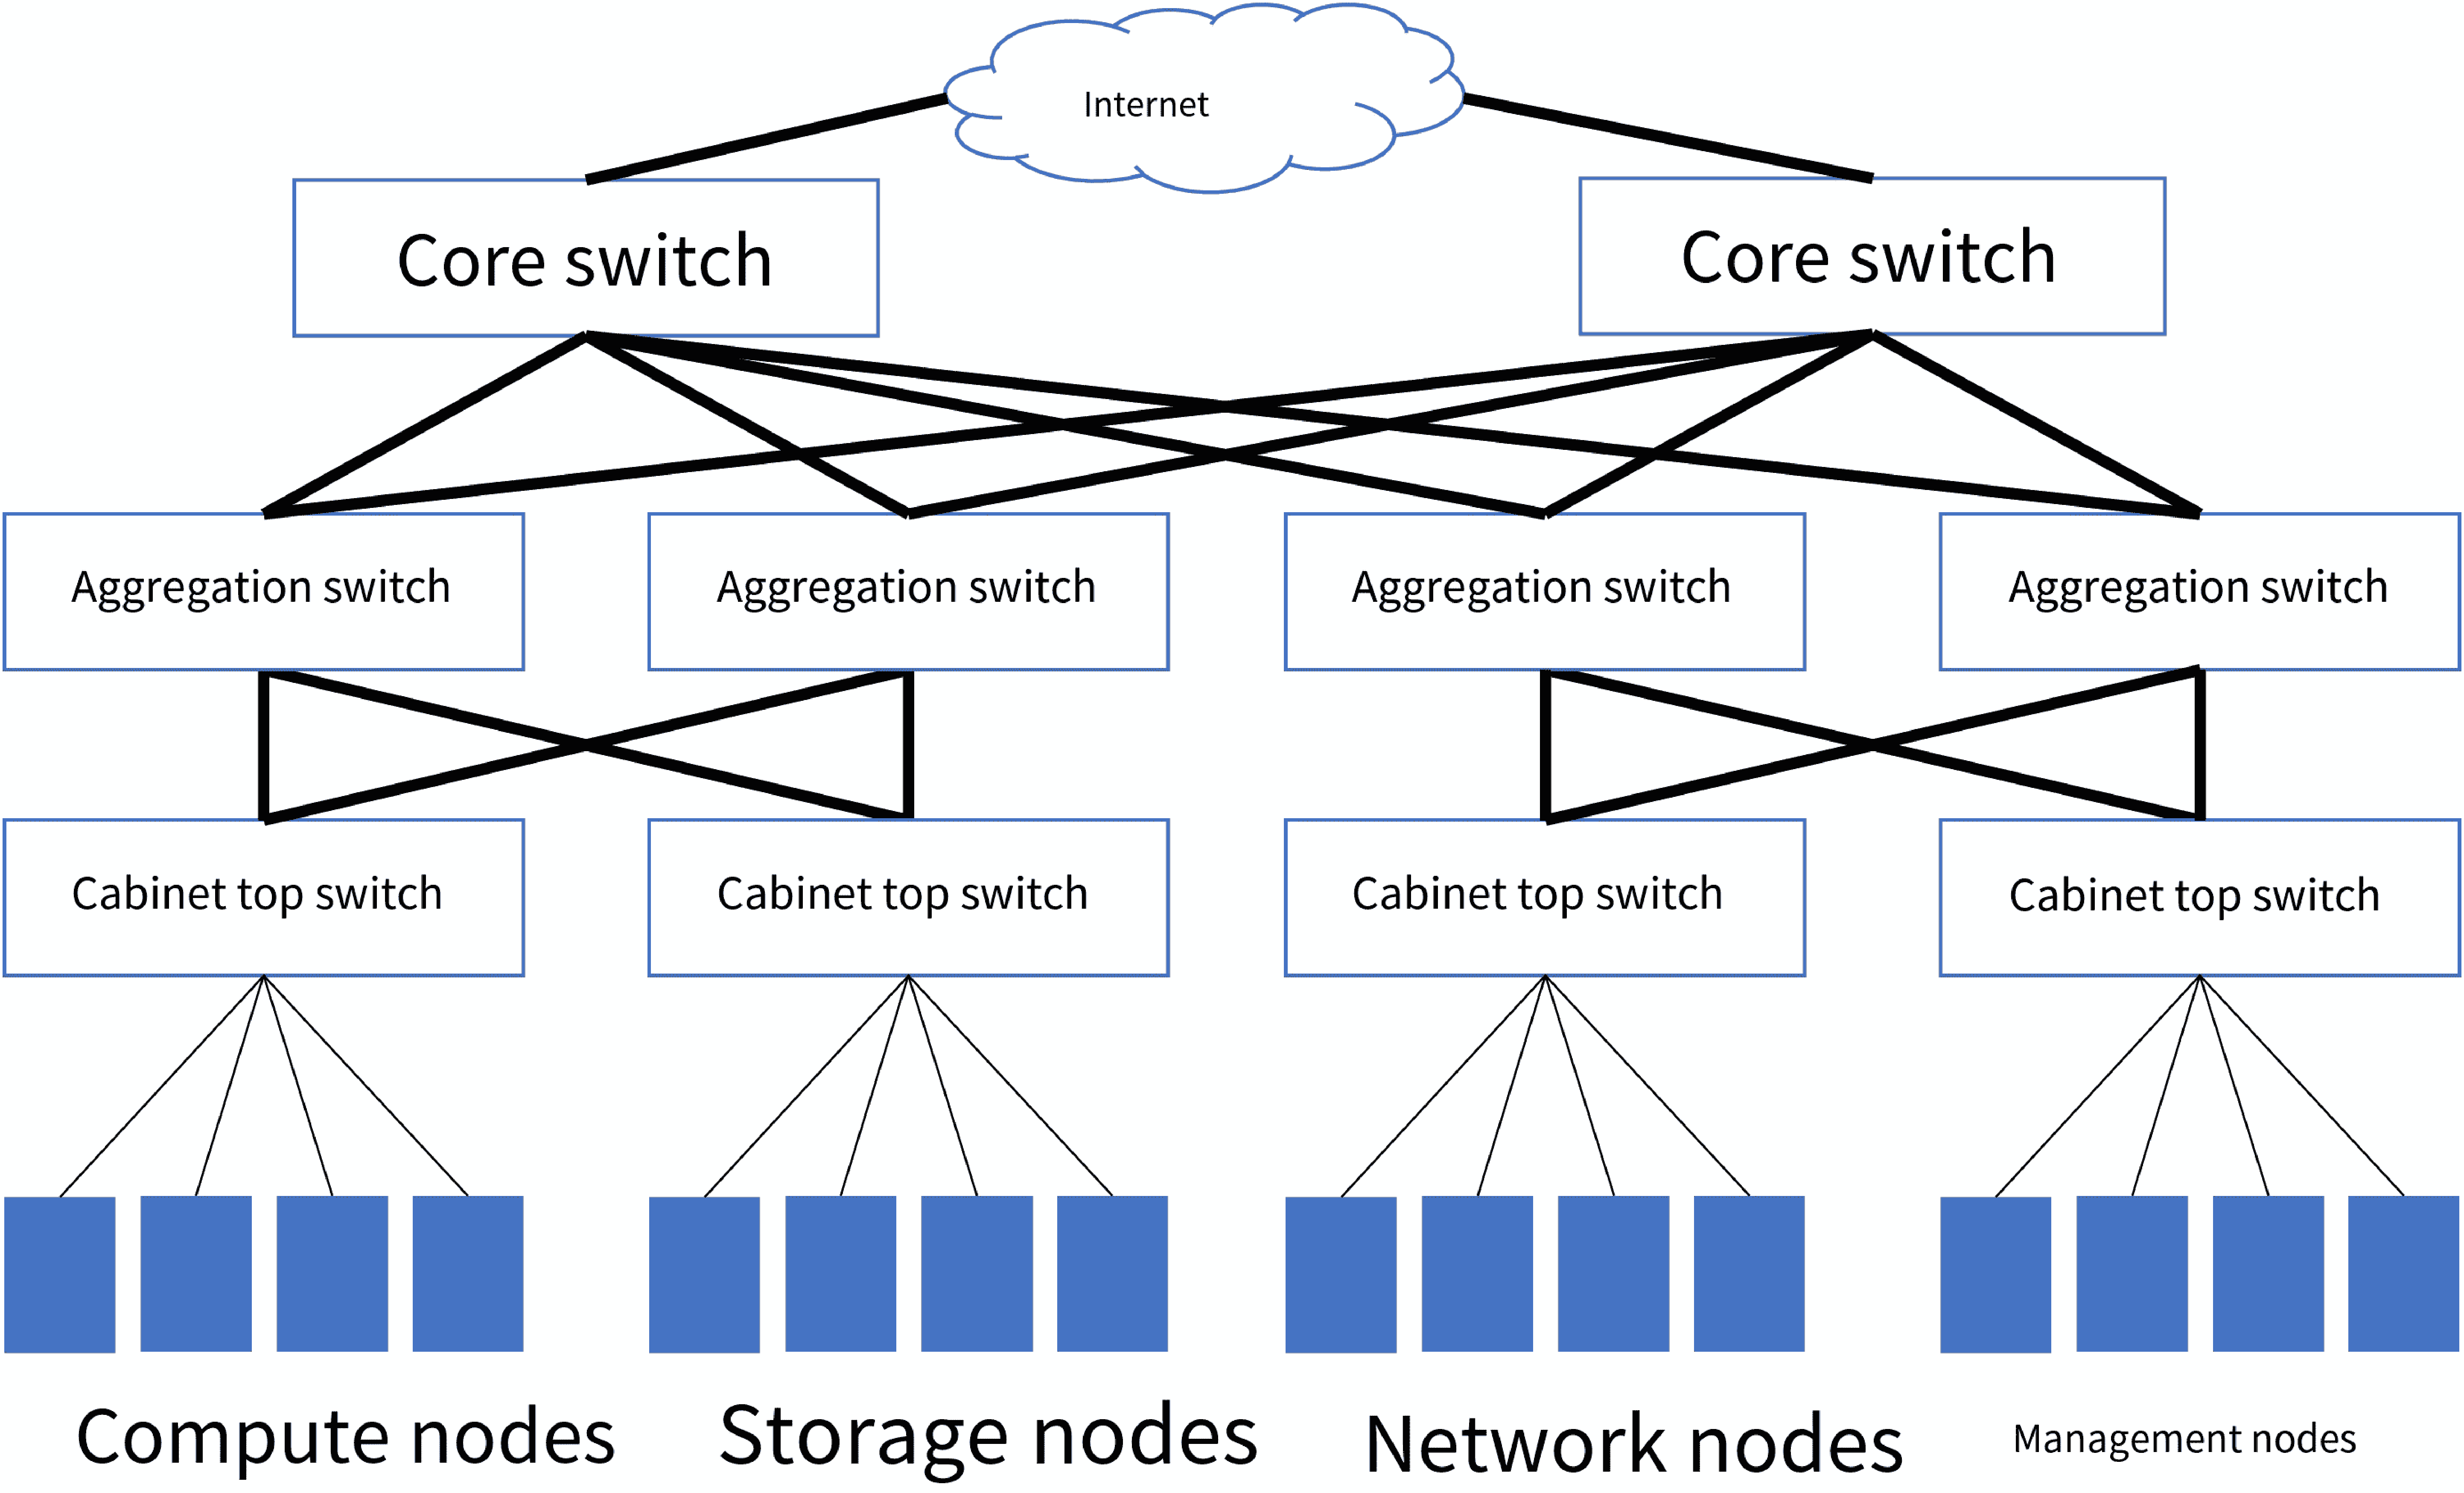
\includegraphics[width=0.6\textwidth]{figures/DC_arch.pdf}
	\caption{数据中心架构。}
	\label{background:fig:cloud-architecture}
\end{figure}

\begin{figure}[htbp]
	\centering
	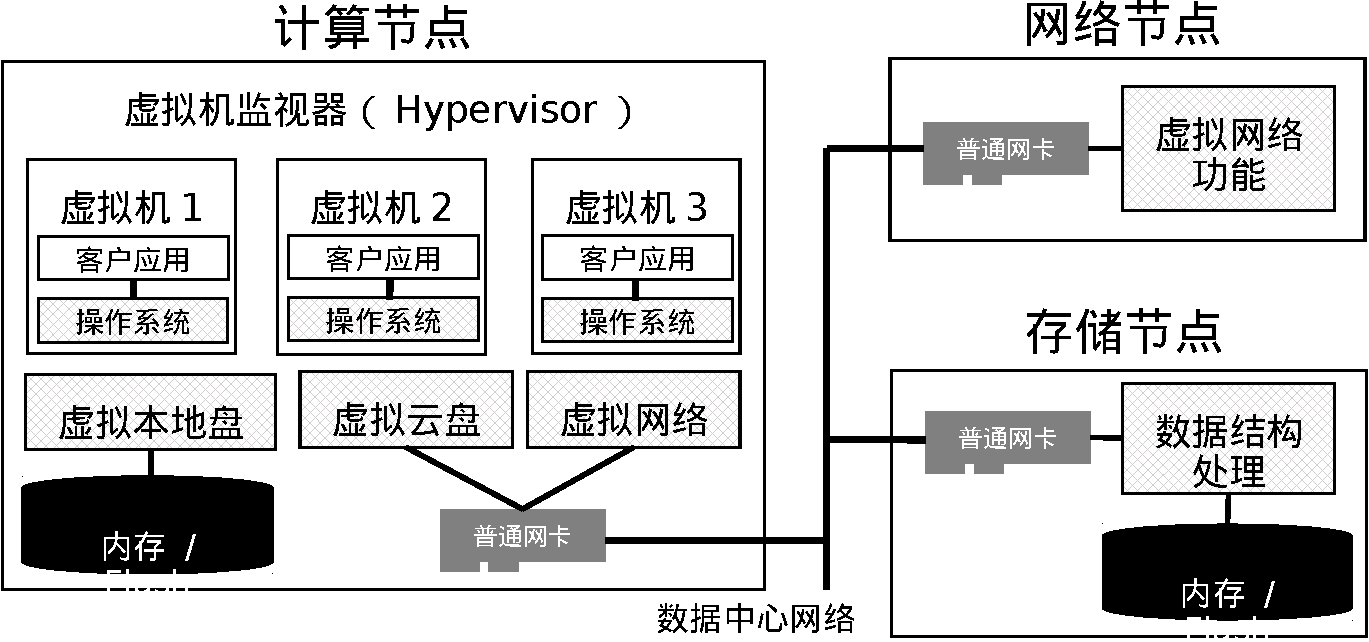
\includegraphics[width=0.8\textwidth]{figures/virt_arch.pdf}
	\caption{虚拟化的数据中心架构。}
	\label{background:fig:virt-architecture}
\end{figure}


\subsubsection{虚拟网络}


公有云中的大客户不再只是需要虚拟机,而是需要模拟企业网络的架构。
为了支持安全组、访问控制列表等网络安全功能,以及在 Internet 中隐藏内部网络结构、减小攻击面,公有云服务提供了虚拟网络(Virtual Private Cloud,VPC)服务,即在公有云中划分出一个逻辑隔离的部分,提供丰富的网络语义,例如具有客户提供的地址空间的私有虚拟网络,安全组和访问控制列表(ACL),虚拟路由表,带宽计量,服务质量保证(QoS)等。 
为此,公有云中的网络被虚拟化了,虚拟网络和物理网络实现了解耦。
如图 \ref{background:fig:network-architecture} 所示,两个计算节点上的客户虚拟机之间通信时,需要经过虚拟网络软件的封装和解封装,还可能需要经过网络节点上的若干网络功能的处理。网络功能将是下一节讨论的主题。

\begin{figure}[htbp]
	\centering
	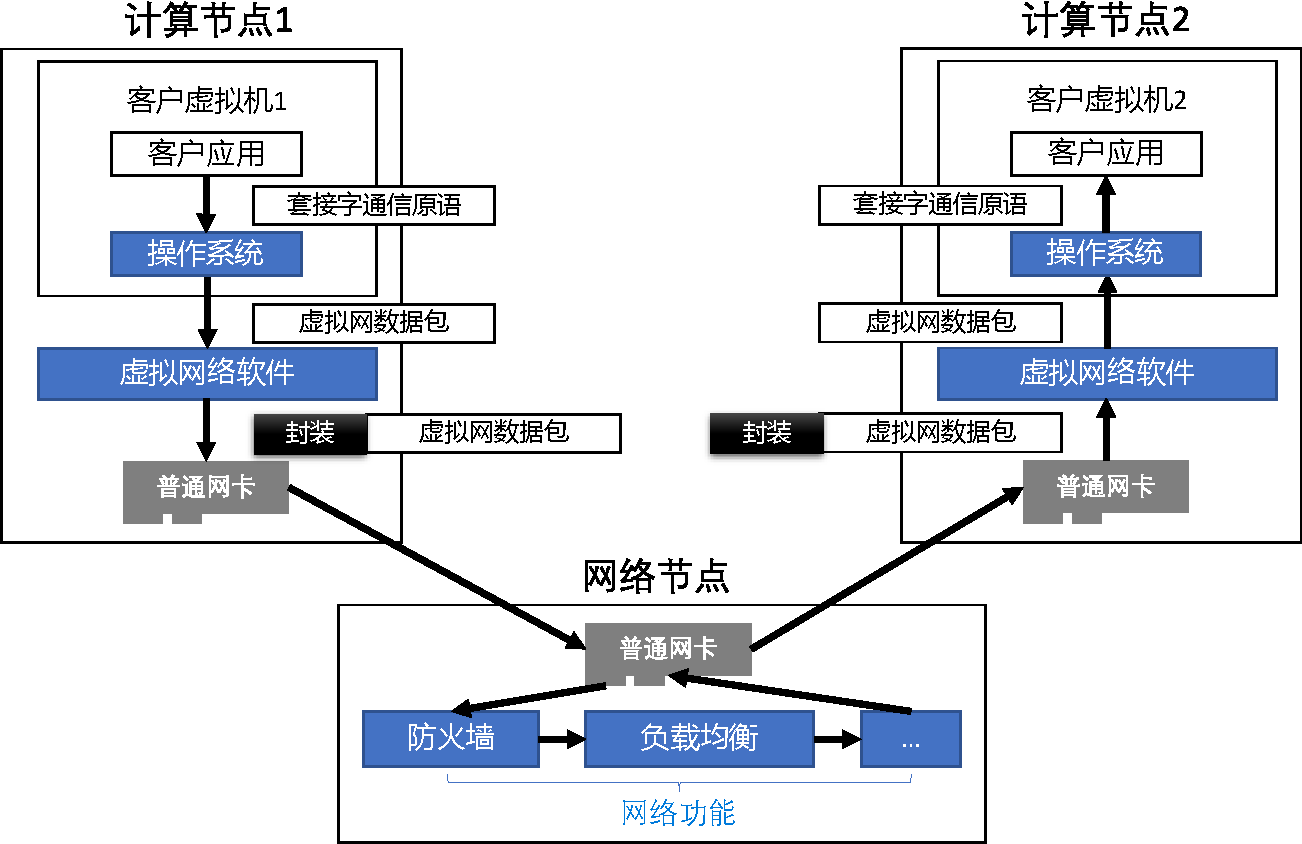
\includegraphics[width=0.8\textwidth]{figures/VPC_arch.pdf}
	\caption{数据中心虚拟网络架构。}
	\label{background:fig:network-architecture}
\end{figure}


虚拟网络的数据面可以用匹配-操作表(Match Action Table)来描述,理论上可以在商用网络交换机上实现。
2007 年,斯坦福大学提出的 OpenFlow \cite{mckeown2008openflow} 统一了不同厂商交换机的控制面接口,从而可以用软件来对网络进行编程,即软件定义网络(Software Defined Networking,SDN)。
为了支持软件定义网络的控制面,Onix \cite{koponen2010onix} 提出了一个大规模交换机的控制框架,Frenetic 等编程语言 \cite{voellmy2010nettle,foster2011frenetic} 提出用函数式响应型编程(Functional Reactive Programming,FRP)的范式简化控制面事件处理,Covisor \cite{jin2015covisor} 实现了控制面的虚拟化。
随着交换机的可编程性越来越高,用软件自顶向下地定义交换机的数据面转发行为成为可能,而不是像 OpenFlow 那样自下而上地适配交换机的固定功能。

为此,2013 年,斯坦福大学提出了 P4 \cite{bosshart2014p4},提供可编程的数据包解析、有状态的匹配-操作流水线等编程抽象。
学术界提出了 P4 语言在可编程交换机芯片 \cite{bosshart2013forwarding}、可编程网卡 \cite{kaufmann2016high}、FPGA \cite{wang2017p4fpga}、CPU 虚拟交换机 \cite{shahbaz2016pisces} 上的多种实现。
工业界的 Barefoot Tofino 交换机芯片 \cite{barefoot-tofino}、Mellanox Connect-X 网卡 \cite{mellanox}、基于 FPGA 的 Xilinx SDNet 网络处理器 \cite{xilinx-p4} 等也支持了 P4 语言。

然而,基于网络交换机的虚拟网络在云数据中心中有两个根本挑战。
首先,实际云数据中心虚拟网络的语义非常复杂,而且变化太频繁,以至于固定功能的传统交换机硬件更新的速度很难匹配需求变更的速度。
其次,一台柜顶交换机连接了数十台机架服务器,一台机架服务器又可以虚拟化出数十台虚拟机,因此交换机需要支持至多上千台虚拟机的数据面封装和转发规则,现有商用交换机芯片的查找表容量不足。
为此,微软提出了类似 P4 的 VFP 编程抽象 \cite{firestone2017vfp} 以支持基于主机的软件定义网络,在虚拟交换机软件中实现虚拟网络。基于主机的虚拟网络可以很好地随计算节点服务器的数量扩放,并保持了物理网络的简单性。

在这种基于虚拟交换机的网络虚拟化模型中,进出物理设备的所有网络I / O都专门在管理程序的主机软件分区中执行。 虚拟机发送和接收的每个数据包都由主机网络堆栈中的虚拟交换机(vSwitch)处理。 接收数据包通常涉及管理程序将每个数据包复制到虚拟机可见的缓冲区,模拟虚拟机的软中断,然后允许虚拟机的操作系统堆栈继续进行网络处理。 发送数据包类似,但顺序相反。 与非虚拟化环境相比,这种额外的主机处理会降低性能,需要对权限级别进行额外更改,降低吞吐量,增加平均延迟和延迟变化,并提高主机CPU利用率。

如图 \ref{background:fig:network-perf-trend} 所示,数据中心网络性能的提升速度远远超过通用处理器,在 10 Gbps 网络中只需要一个 CPU 核,而在现在的 40 Gbps 网络中就需要 5 个左右的 CPU 核,而在未来的 100 Gbps 网络中甚至需要 12 个 CPU 核。这就带来了 ``数据中心税''。





\begin{figure}[htbp]
	\centering
	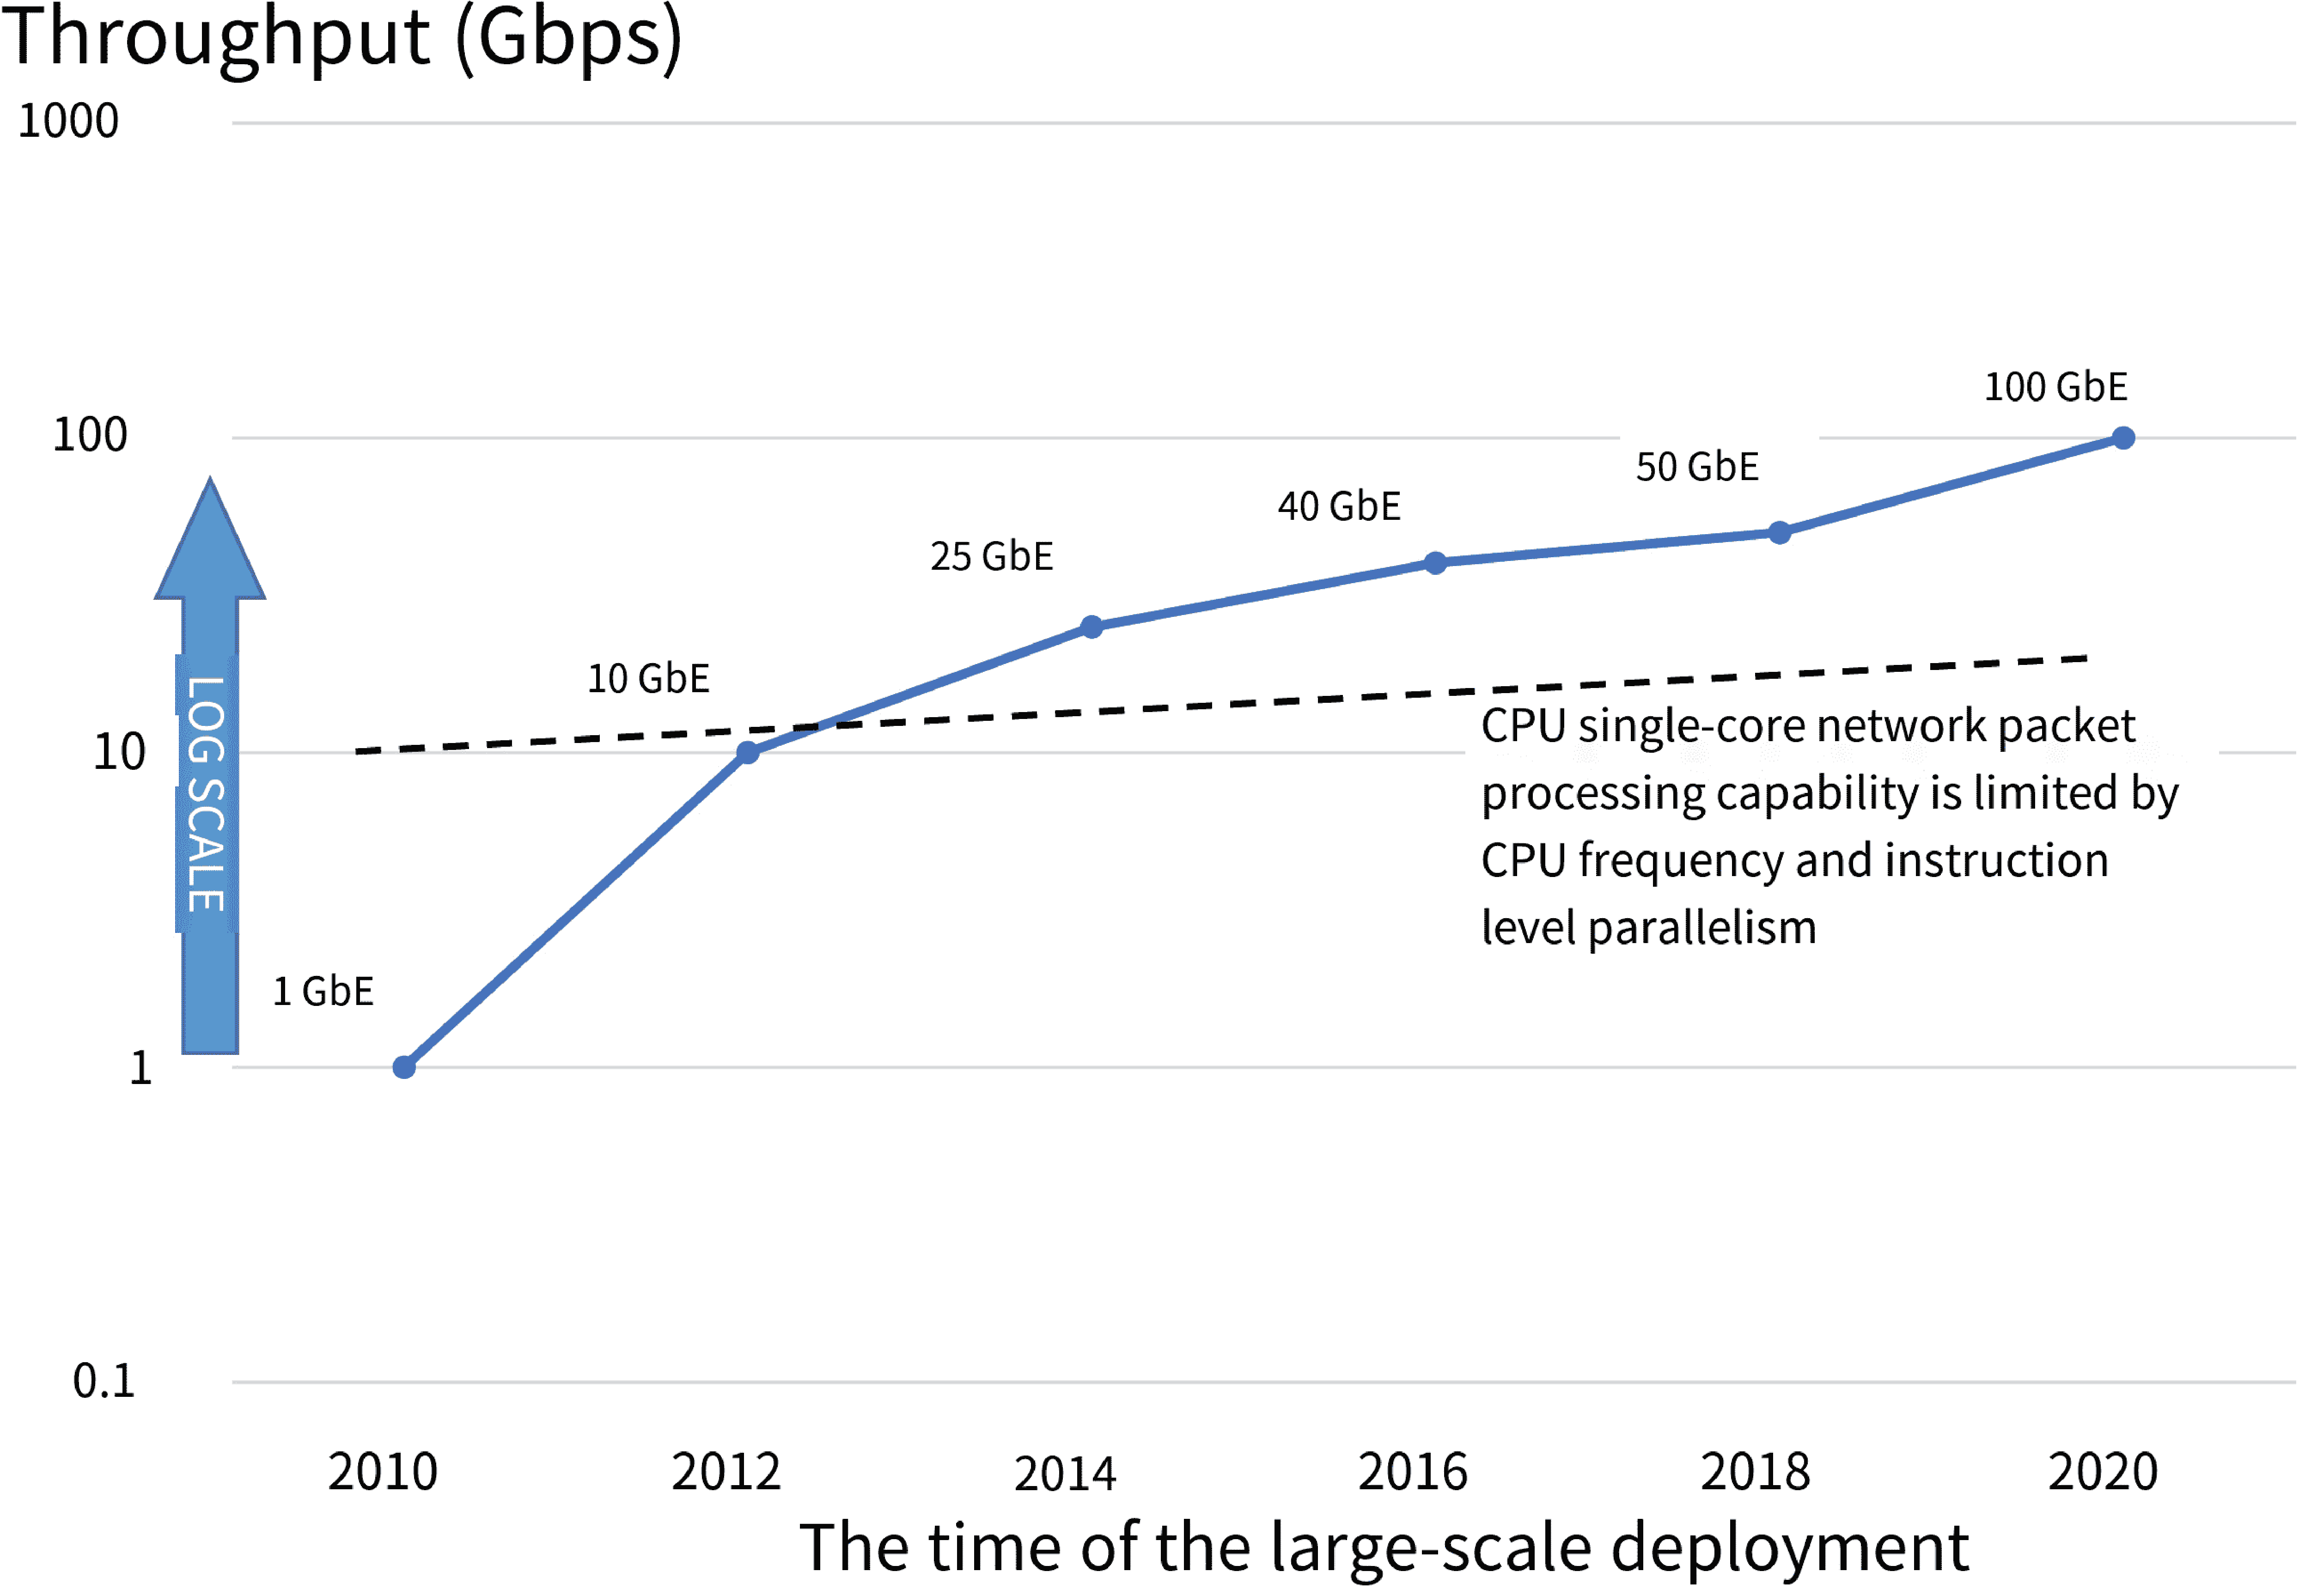
\includegraphics[width=0.6\textwidth]{figures/network_perf_trend.pdf}
	\caption{数据中心网络性能的提升速度远超 CPU。}
	\label{background:fig:network-perf-trend}
\end{figure}


\subsubsection{网络功能}

除了虚拟网络,数据中心还需要多种网络功能。
例如,大型互联网服务有多台前端服务器并发处理用户请求,这就需要一个高可用、高性能的负载均衡器接受用户的请求,并分发到前端服务器上。
企业级负载均衡器还可能支持一系列高级功能,例如基于用户请求的灵活负载均衡规则,HTTPS 安全连接,日志记录和统计,检测并过滤可能的拒绝服务(DoS)攻击、注入攻击等 \cite{ananta}。
再如,很多政府和企业已经有自己的 IT 信息系统,如果全部迁移到公有云上,就不符合一些机构对数据隐私和安全的要求,一次性迁移的成本和风险也过高。
因此,连接客户已有的 IT 信息系统(on-premises)和公有云上的虚拟网络就是很必要的。
此外,针对客户对数据安全和隐私的顾虑,很多云厂商提供了私有云(或称专有云)模式,也就是把公有云的软硬件架构部署到客户专属的数据中心基础设施上。
为了支持办公场所(on-premises)、私有云和公有云之间的连接,云厂商需要提供虚拟专线服务,这就需要能实现加密、路由、访问控制列表等基础网络功能以及缓存、TCP 加速等高级网络功能的专线网关。在一些情况下,这些云之间和云与办公场所之间的连接不是通过 SDH 或 MPLS 专线,而是通过 Internet 公共互联网。此时就需要用 IPSec 等协议对数据进行加密和签名,使用的是 IPSec 网关 \cite{son2017protego}。

通过负载均衡器和专线 / IPsec 网关这两个例子,可以看到,网络功能的复杂程度明显高于虚拟网络。
虚拟网络运行在网络层、数据链路层,一般只需要处理数据包头部信息,且不需要维护复杂的可变状态;而网络功能覆盖了应用层、传输层、网络层等,需要处理数据包的有效载荷(payload),且需要根据数据包查找到所属网络连接,根据连接的当前状态做出处理,再更新连接的状态。
P4 \cite{bosshart2013forwarding} 的编程灵活性不足以实现灵活的数据包有效载荷处理和基于连接的有状态处理。
Click \cite{kohler2000click} 提出了模块化的路由器编程框架,比较适合灵活的网络功能处理。
近年来,ClickOS \cite{martins2014clickos} 和 NetBricks \cite{netbricks} 等一系列工作改进了 Click 在 CPU 上的性能。
E2 \cite{palkar2015e2} 提出了高可用、高可扩放性的网络功能调度和管理框架。
本文第 \ref{chapter:clicknp} 章将提出一个基于 FPGA 的高性能网络功能处理平台,实现了基于 Click 的高级语言模块化 FPGA 编程。







\subsubsection{虚拟存储}

云计算中的虚拟存储由本地存储和远程存储两部分构成。
远程存储则是由存储节点虚拟出的分布式存储系统,提供高可靠性、高可用性、容量可扩放性和吞吐量可扩放性,是云平台中的主要存储方式。
本地存储包括非易失性内存(Non-Volatile Memory,NVM)和 NVMe 高速闪存盘(flash storage),主要用于需要极致性能,但数据不需要高可靠性存储的分布式数据库等应用。

虚拟存储提供给客户的最基本服务是块存储(block storage),可以作为块设备(block device)挂载到虚拟机作为磁盘使用。
云服务还提供了对象存储(object storage)、文件存储(file storage)等存储服务。
这类服务大多提供类似键-值(key-value)映射的抽象,即用户指定键,读取(GET)或写入(PUT)相应的值。
键-值存储作为一种基础数据结构,可以分为持久化存储、临时存储;根据是否需要复制和容灾,是否支持事务(transaction),提供强一致性或最终一致性 \cite{anna},是否支持范围索引、二级索引、内容索引等,可以组合出形形色色的存储系统,满足不同应用的需求。

虚拟存储系统的两个基本逻辑概念是客户端和服务器。
如图 \ref{background:fig:storage_arch} 所示,客户端是云存储服务的使用者,如云上承载客户虚拟机的计算节点;服务器提供块存储、对象存储、文件存储等抽象,把逻辑存储的读写请求映射到物理存储介质的读写请求。
多个客户端可能共享同一个虚拟存储,例如分布式数据处理系统中的多个计算节点可能需要访问共享的原始数据和配置参数,数据处理的中间结果也可以通过存储来传递。
同一个虚拟存储可能对应多个存储服务器,用于实现存储的容量可扩放性、吞吐量可扩放性、容错和高可用。


\begin{figure}[htbp]
	\centering
	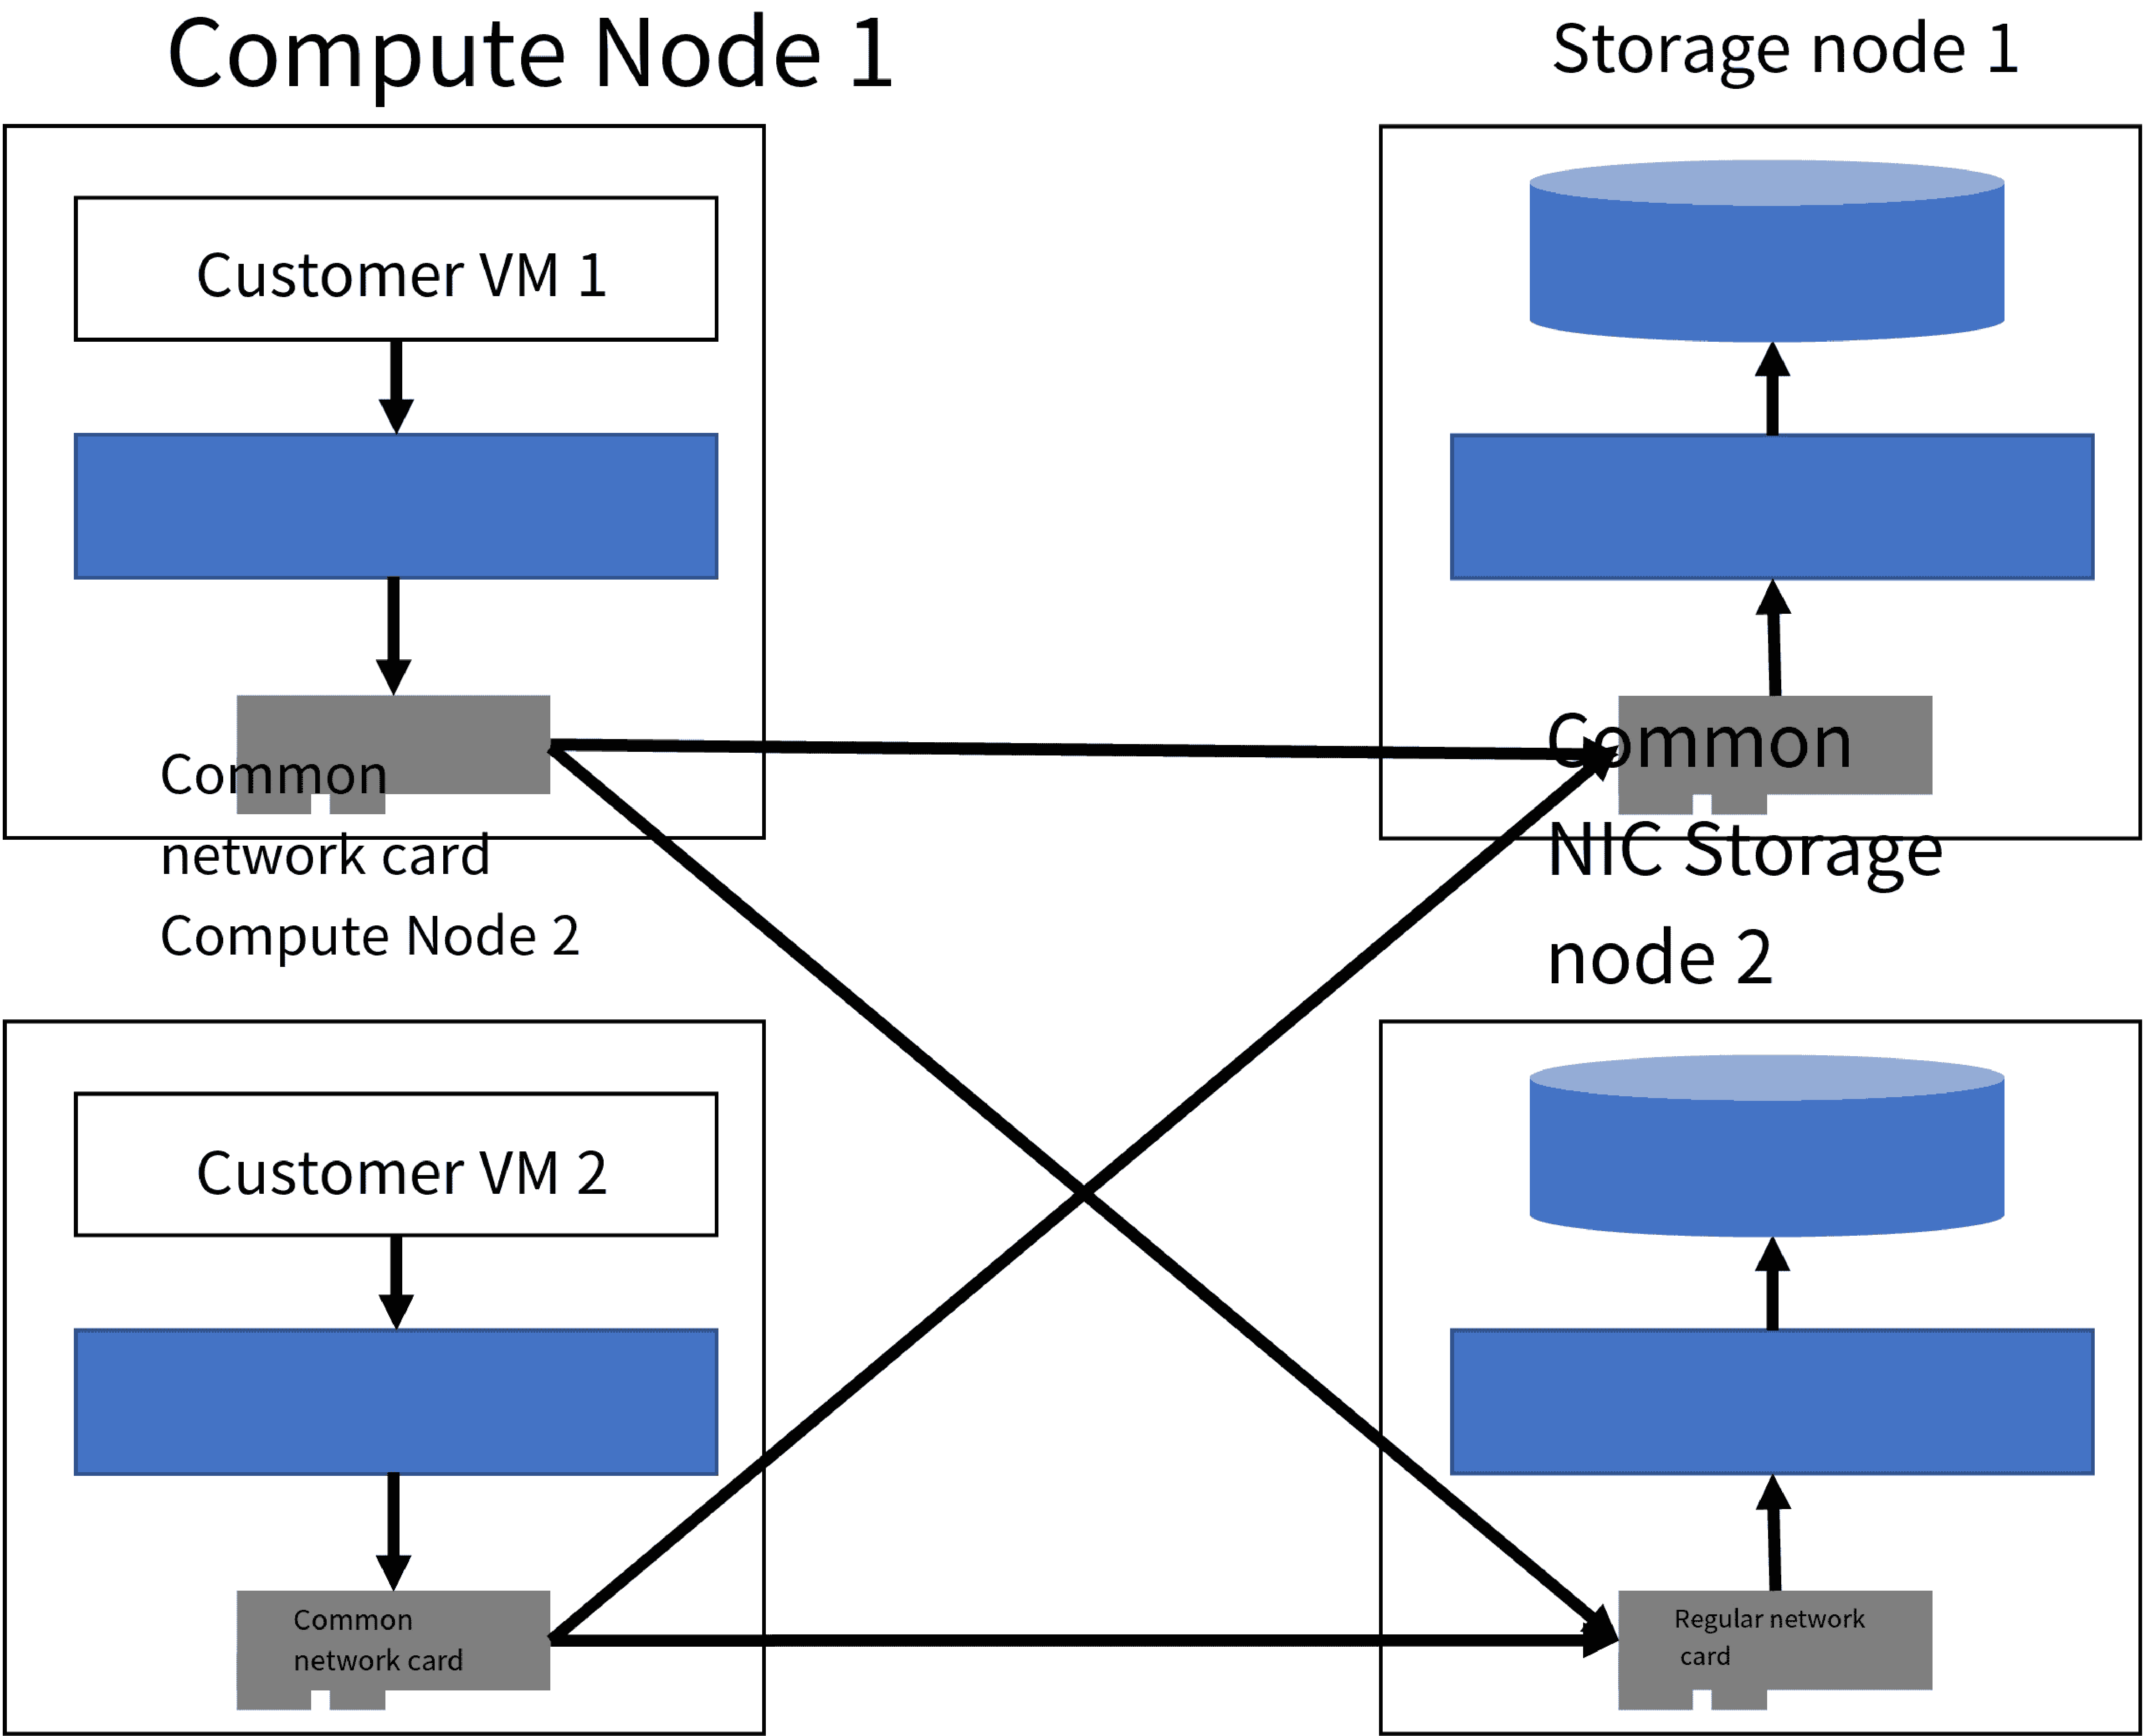
\includegraphics[width=0.6\textwidth]{figures/storage_arch.pdf}
	\caption{数据中心云存储的简要架构。}
	\label{background:fig:storage_arch}
\end{figure}


上述存储服务器的结构是较为简化的,事实上往往分为多个层次。
例如,微软 Azure 的云存储服务分为前端节点、中间节点和后端节点 \cite{calder2011windows}。
前端节点负责解析和验证请求,并根据数据分片映射表(例如键的哈希值),分发到数据所在分片的中间节点。中间节点负责实现请求的处理和存储数据结构的处理,把用户的请求映射成一系列存储读写操作,分发给对应的后端节点。后端节点负责实现数据的复制(replication)以及在物理介质上的存储。

在数据中心中,由于存储服务器需要安装较大容量的存储介质,存储节点的硬件配置一般与计算节点是不同的。此外,计算节点上由于运行客户的虚拟机,虚拟机监控器软件经常需要升级以增加新功能和修补安全漏洞,因此计算节点的稳定性通常比存储节点低。为了保证存储的高可用性,存储节点与计算节点通常是分离在不同物理主机上的。因此,计算节点上的存储客户端通常需要把数据从存储服务器通过网络搬运过来。
也就是说,客户虚拟机的每个 I/O 请求都需要被虚拟机监控器捕获,然后从计算节点上虚拟机监控器内的存储客户端软件出发,依次经过存储服务器的前端、中间和后端节点的处理,才能到达存储介质。
为了保证数据的安全性,物理存储介质上的数据一般需要加密存储。为了节约存储空间,降低单位存储容量的存储介质成本,很多云厂商还会对存储的内容进行压缩。压缩和加密一般在存储服务器上进行,属于计算密集型操作。例如,根据实验,在 LZ77 较好的压缩率下,一个服务器 CPU 核心每秒通常只能压缩 100 MB 的数据;对 1 KB 的块,AES 加密和 SHA-256 签名每秒也只能处理 100 MB 的数据。

由于软件处理和网络传输的开销,云计算平台上块存储的延迟一般为 0.5 至 1 毫秒,对象存储的延迟一般为 1 至 10 毫秒 \cite{jonas2019cloud},远高于物理存储介质的延迟(如 SSD 的延迟一般为 0.1 毫秒)。
此外,云存储的吞吐量也低于相应的物理存储介质,例如 SSD 云盘最高的吞吐量为 50 K 次 I/O 每秒,而单块数据中心级 SSD 的吞吐量就已达数百 K 次 I/O 每秒 \cite{jonas2019cloud}。
为了充分利用最新的数据中心存储硬件的性能,云存储服务需要全栈优化。
例如,很多数据中心在存储协议栈的网络传输方面,已经使用 RDMA 协议降低了网络协议栈的 CPU 开销和延迟 \cite{guo2016rdma}。
一些数据中心还通过改进云存储的协议栈,把客户端、服务器前端、中间、后端节点的功能进行适当的整合,减少层次 \cite{nitro-blog}。
本文将提出一种数据面完全由可编程网卡处理的云存储架构,把软件处理的 CPU 和延迟开销尽可能降低。


\subsubsection{内存数据结构存储}

云存储通常是指持久化存储。在分布式系统中,内存数据结构存储(in-memory data structure storage)也很重要。传统上,内存数据结构存储主要用于缓存,例如经常访问的网页内容和实时更新的排行榜。Memcached \cite{memcached}、Redis \cite{redis} 是被广泛使用的内存数据结构存储软件,大多数主要提供键-值(key-value)映射的数据结构,并在其基础上扩展出队列、数组、优先队列等更复杂的数据结构。

随着大规模分布式计算变得越来越重要,内存数据结构存储作为进程间通信的两种范式(消息传递和共享内存)之一,成为分布式计算的重要基础组件。
例如,大数据处理的框架 Spark 把内存键-值存储作为数据处理中间结果的存储和传递方式,一方面用于把计算流图中前驱节点的计算结果作为后继节点的输入;另一方面用于在计算节点出现故障时从前驱节点的输出恢复,重新执行后继节点的计算。
图计算(graph computing)\cite{wu2015g,xiao17tux2} 中的分布式计算节点共享同一张图,图中的点、边等信息就可以使用键-值映射来表达。

分布式机器学习训练中,数据并行是常见的范式。基于同步随机梯度下降(SGD)方法的分布式机器学习训练由若干阶段(epoch)构成,每一阶段开始时,各个计算节点之间共享一个模型,并使用不同的训练数据分别计算出模型的梯度,然后把各个计算节点的模型梯度汇总起来,修改模型,作为下一阶段各个计算节点的共享模型 \cite{distributed-ml}。为了便于分发模型和汇总模型的梯度,分布式机器学习训练系统常常配备一个分布式的参数服务器(parameter server) \cite{li2014scaling},相当于共享内存。
近年来开始流行的异步随机梯度下降和半同步随机梯度下降训练方法中,也需要把每个节点产生的梯度分发到所有节点,参数服务器仍然是解决参数同步问题的常用方法。
分布式强化学习框架 Ray \cite{moritz2018ray} 通过键-值存储来保存数据流处理过程的中间状态。

作为最后一个例子,分布式数据库中,为了事务的并发控制,分布式数据库系统往往给每个事务分配一个递增不重复的序列号 \cite{li2017eris},该序列号发生器也是键-值存储的应用场景。

未来,内存数据结构存储还将成为赋能无服务器计算(serverless computing)的基础服务。无服务器计算中,函数应当是无状态的,有状态应用就需要把状态存储到外部存储中,多个函数组成的计算流图也需要外部存储来传递中间结果。如果使用持久化存储,尤其是现有的云存储,其性能和成本都是不可接受的 \cite{jonas2019cloud}。

\begin{figure}[htbp]
	\centering
	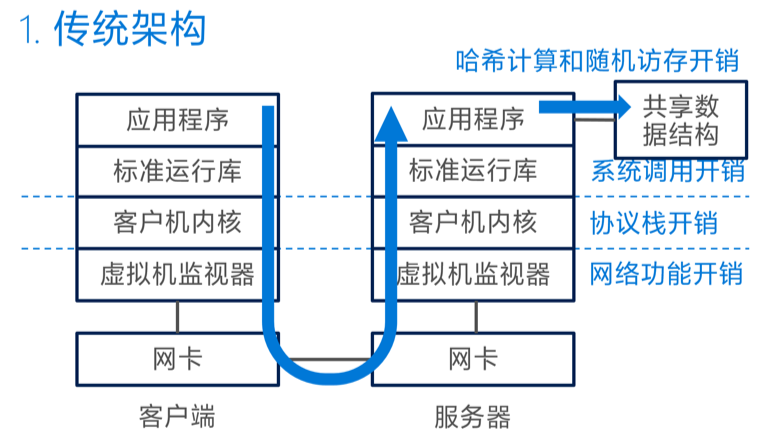
\includegraphics[width=0.6\textwidth]{figures/kvdirect_traditional.png}
	\caption{传统基于软件的内存数据结构存储系统架构。}
	\label{background:fig:kvdirect_traditional}
\end{figure}

如图 \ref{background:fig:kvdirect_traditional} 所示,传统基于软件的内存数据结构存储系统在客户端和服务器端都需要跨越标准运行库、操作系统内核、虚拟机监视器等多个层次,还需要通过软件处理共享数据结构的并发访问,带来一系列开销。
本文第 \ref{chapter:kvdirect} 章将提出基于可编程网卡的内存数据结构存储,具有高吞吐量、低延迟、延迟稳定的特点。
内存数据结构存储作为数据中心的重要基础服务,在分布式计算规模不断扩大、编程粒度逐渐缩小的趋势下,发挥越来越重要的作用。

\subsubsection{操作系统}

``数据中心税'' 的最后一个方面是操作系统的开销,主要是指操作系统处理 I/O 操作的开销。
在本文中,网络和存储操作统称 I/O 操作。
以网络操作为例,分布式应用程序基于消息传递范式的进程间通信普遍使用操作系统中的套接字(socket)原语。
如图 \ref{background:fig:kernel_time} 所示,对于 HTTP 负载均衡器、DNS 服务器、Memcached \cite{memcached} 和 Redis \cite{redis} 键-值存储服务器等通信密集型的应用程序,操作系统占用了 50\% 至 90\% 的 CPU 时间,大部分用来处理套接字操作。


\begin{figure}[htbp]
	\centering
	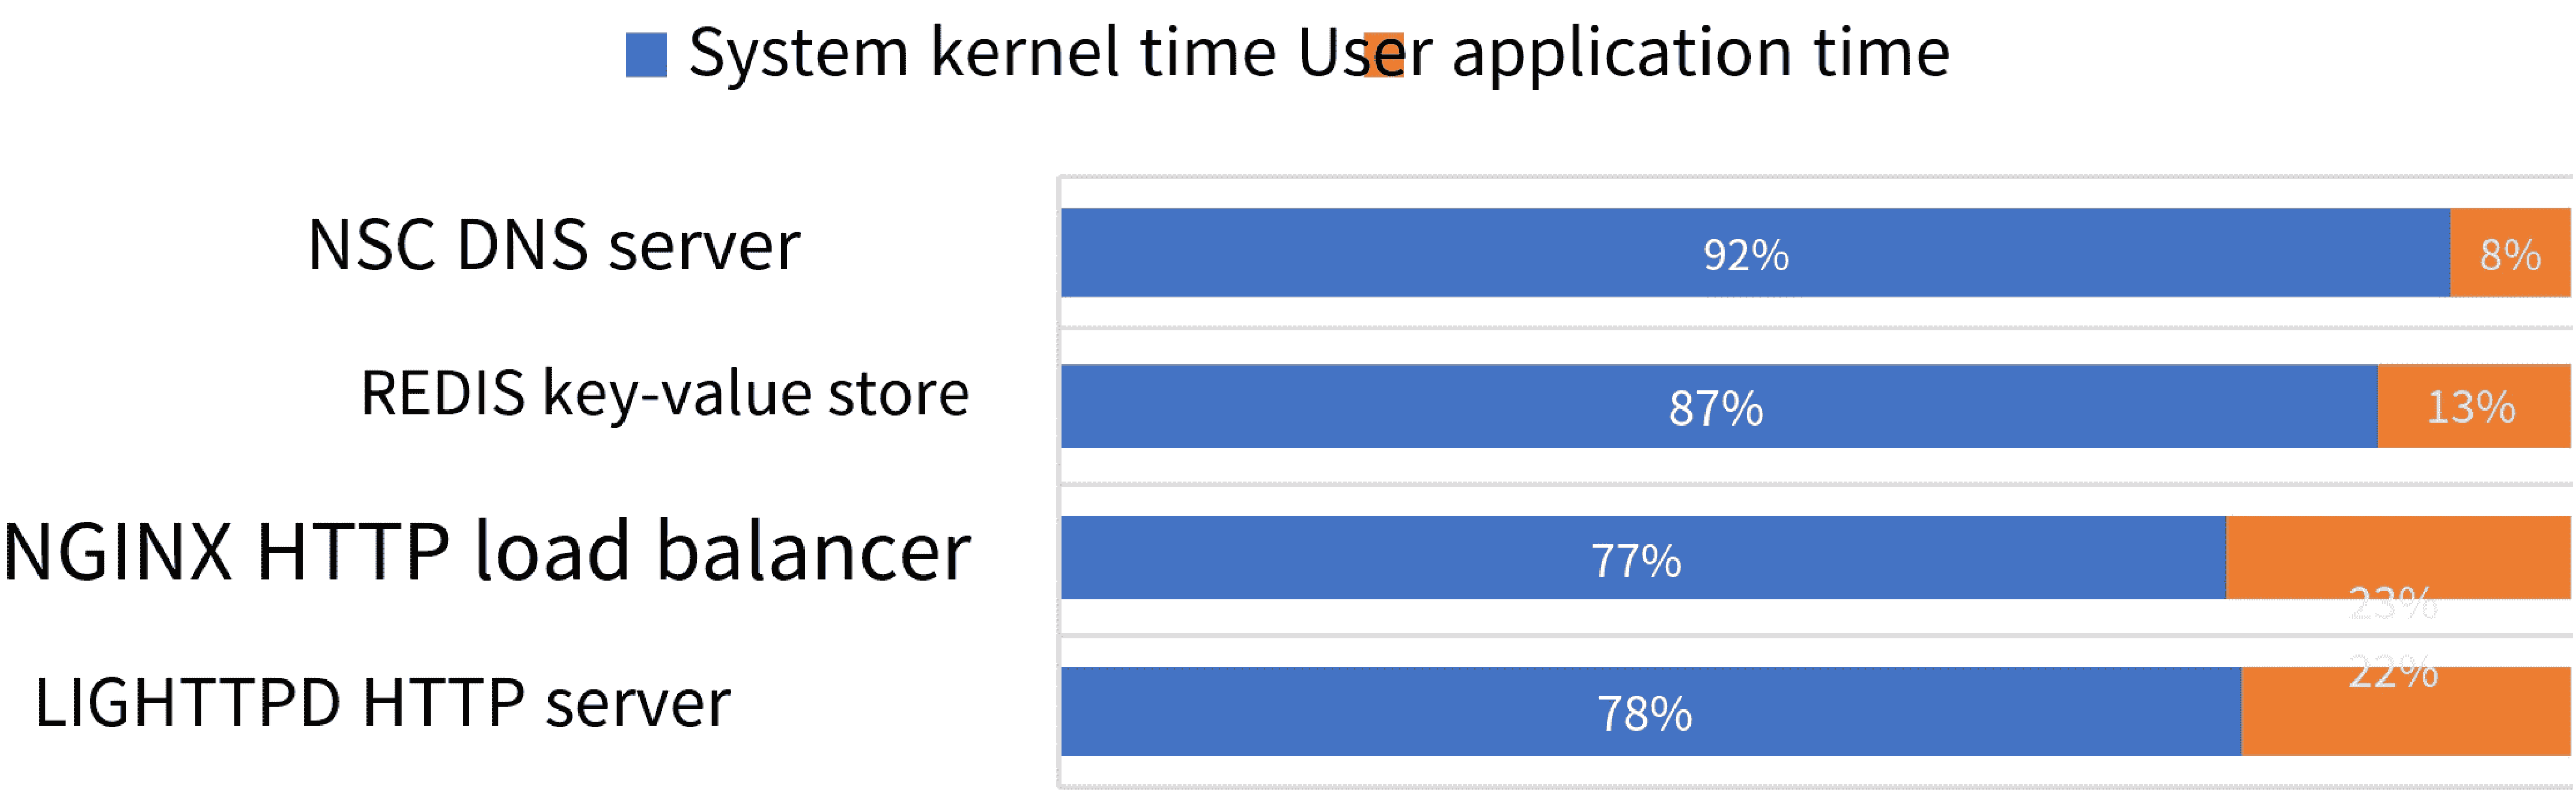
\includegraphics[width=0.8\textwidth]{figures/kernel_time.pdf}
	\caption{通信密集型应用程序在操作系统内核中消耗了大量的 CPU 时间。}
	\label{background:fig:kernel_time}
\end{figure}

在 Linux 操作系统中,应用程序通过文件描述符(File Descriptor,FD)进行 I/O 操作。
从概念上讲,Linux 网络协议栈由四层组成。首先,虚拟文件系统(VFS)层为应用程序提供基于文件描述符的套接字 API。
其次,在传输层,传统的 TCP 传输协议提供I / O复用,拥塞控制,丢包恢复等功能。
第三,在网络和链路层,IP 协议提供了路由功能,Ethernet 提供了数据链路层的流控和物理信道复用,Linux 还实现了服务质量保证(QoS)和基于 netfilter 框架的防火墙等。
第四,在设备驱动层,网卡驱动程序与网卡硬件(或用于主机内套接字的虚拟环回(loopback)接口)通信以发送和接收数据包。

众所周知,虚拟文件系统层贡献了网络 I/O 操作的很大一部分开销 \cite {clark1989analysis,boyd2010analysis}。
在本文第 \ref{chapter:socksdirect} 章中,将通过一个简单的实验来验证:主机中两个进程之间的Linux TCP套接字的延迟和吞吐量只比 Linux 管道(pipe)、FIFO和Unix域(domain)套接字稍差。
管道,FIFO和UNIX域套接字绕过了传输层和网卡层,但它们的性能仍然不尽如人意。

以 Linux 网络协议栈为例,其开销是多方面的。对每次 I/O 操作,都需要进行内核穿越(kernel crossing),还需要获取文件描述符锁以保护多线程并发操作。每发送和接收一个数据包,都涉及到传输协议、缓冲管理、I/O 多路复用、中断处理、进程唤醒等一系列操作系统开销。每发送和接收一个字节,其内存都要复制数次。每建立一个 TCP 网络连接,都要分配内核文件描述符、TCP 控制块,TCP 服务器端还要对新连接进行调度。这些开销将在第 \ref{chapter:socksdirect} 章详细讨论。

本文第 \ref{chapter:socksdirect} 将提出一个用户态网络协议栈,将操作系统的网络协议栈开销转移到用户态库和可编程网卡,实现接近硬件性能的网络传输。


Linux 存储协议栈逻辑上由五层构成。首先,是与网络协议栈类似的虚拟文件系统层,提供基于文件描述符的 API。
其次,文件系统层实现文件系统的抽象,提供文件的路径查找、权限管理、空间分配等功能。
第三,缓存缓冲层与 Linux 的内存管理机制紧密结合,负责管理读缓存和写缓冲,以及页面换入换出机制。
第四,块设备层把存储设备抽象为若干个 ``块''(block),实现块访问的合并、排序等。
第五,在设备驱动层,存储介质驱动程序与硬件通信以读取和写入硬盘块。
在存储协议栈中,虚拟文件系统层也是开销的重要来源。对数据库等很多使用直接 I/O 的应用,文件系统、缓存缓冲层是不必要的。
将用户态网络协议栈扩展到包括存储在内的所有 I/O 操作将是未来的方向。

\subsection{数据中心功耗的挑战}

如今的一个大型数据中心可以占据几个足球场的面积,容纳数十万台服务器,消耗几十甚至上百兆瓦的电力,相当于一个小型工业城镇的耗电量。据统计,2018 年全球数据中心约消耗 416 太瓦时的电力,相当于 2\% 左右的全球电力能源 \cite{datacenter-energy},占整个信息与通信产业(ICT)能耗的约 33\%。据预测,2025 年,信息与通信产业将消耗 17.8\% 至 20.7\% 的全球电力能源,其中数据中心占 43\% 至 58\% \cite{power-consumption},这意味着 2025 年数据中心将消耗全球电力的约 10\%。因此,数据中心的性能与效率不仅关系到互联网公司的资产和运营成本,还关系到信息产业的未来。

为什么能源问题对信息产业的未来如此重要呢?
1961 年,钱学森预言,``长远以来人们就有在宇宙空间飞行的愿望……星际航行将是科学技术在 20 世纪后半叶中最突出的成就。'' \cite{qianxuesen}
可惜,不同于钱老等大科学家和阿瑟·克拉克等大科幻作家的预言,星际航行的探索尽管推动了众多科学和工程技术的大发展,但由于能源和材料的限制,至今没有成为一项大众技术。
而信息和通信技术(ICT)由于摩尔定律所预言的指数级性能提升,成为 20 世纪末以来最为耀眼的科技新星。

由于信息是无形的,可以通过把信息的存储和处理单元做得越来越小来提升单位面积集成电路的存储和处理单元数量,从而提升单位面积集成电路的性能。这也是摩尔定律的原始表述。
更为深刻的是 Dennard 缩放定律 \cite{dennard1974design},即集成电路的性能在不消耗更多能源和面积的情况下能够每两年翻倍。
它的理论基础是每两年采用一代新的半导体工艺,晶体管尺寸缩小 30\%,从而芯片面积缩小 50\%。为了保持电场的恒定,电压随晶体管尺寸同比例降低了 30\%。与此同时,由于芯片尺寸缩小了,延迟降低了 30\%,时钟频率就可以提升 40\% \cite{borkar1999design,borkar2011future}。
在那个年代,集成电路的动态功耗占了功耗的主要部分,其与电容、电压的平方和频率成正比,从而可以计算出功耗降低了 50\%。
按照这个理想模型,每两年集成电路的面积和功耗都减半,就可以在原有的面积和功耗下塞进两倍数量的晶体管,而且时钟频率还提高到了 1.4 倍。
对于冯·诺伊曼体系结构的单线程微处理器,这些增加的晶体管主要用于更大的缓存、更复杂的流水线、超标量、乱序执行、寄存器重命名、分支预测等,以提高每时钟周期所能执行的指令数。
根据 Pollard 经验定律 \cite{pollackpollack},每时钟周期的计算能力大约与晶体管数量的平方根成正比。
单位时间的算力等于时钟频率乘以每时钟周期的算力,因此每两年微处理器的性能提升到 2 倍,还不消耗更多的能源和面积。

信息系统性能提升的速度在处理宏观有形物体的其他行业是难以想象的。
1976 年,协和式客机的速度就突破了音障,然而它因为油耗太高而没有经济性。现代客机与 50 年前的多数客机一样,仍然以亚音速飞行。
而从普速火车到高铁的大量系统创新,也只把运营速度提高到了 2 倍多。
目前,人类的主要能源来源是化石能源,由于其使用成本和环境影响,在新能源技术取得重大突破前,能源仍然是各行各业发展的重要制约因素 \cite{energy}。
相比数据中心,移动终端和物联网设备对功耗更敏感,因为电池的能量密度提升缓慢,而这些设备对体积和重量很敏感。

不幸的是,进入 21 世纪以来,摩尔定律和 Dennard 缩放定律的红利正在逐渐消失。
首先,随着集成电路特征尺寸的缩小,电压也随之降低。但控制晶体管的阈值电压越低,晶体管的漏电流就会迅速增长,成为集成电路功耗的重要组成部分。
为了控制漏电流,阈值电压不仅不能降低,甚至需要比前一代集成电路有所提高 \cite{borkar1999design}。
因此,每一代新的半导体工艺,每晶体管的功耗不会像预期的那样降低一半。
其次,由于每晶体管的面积缩小一半,功耗却没有降低这么多,单位面积集成电路的功耗就会升高。
目前 100 平方毫米芯片的功耗大约是 65 瓦 \cite{borkar2011future},成为人类最高功率密度的可控设备之一,单位体积的功率密度甚至与航空发动机相当。因此,芯片的散热问题成为制约集成电路规模的主要因素。
再次,对于同一个集成电路,在允许的范围内,为了提高一倍的性能而把时钟频率提高一倍,电压就要相应提高一倍来降低晶体管的翻转延迟,因此功耗大致与时钟频率的三次方成正比。
由于散热的限制,集成电路的时钟频率也受到限制,靠 ``超频'' 来大幅提升集成电路性能是不现实的。
最后,目前 7 nm 半导体工艺已经量产,而硅原子的半径为 0.1 nm。
随着集成电路的特征尺寸越来越接近原子尺寸,量子效应不可忽略,给光刻技术带来了很大的技术挑战 \cite{borkar2011future}。
事实上,约 2010 年以来,集成电路特征尺寸的缩小已经明显放缓,不再能保持两年一代的速度。
综上,在当前的半导体技术框架下,单位面积集成电路的性能已经不再能维持两年提升一倍的速度,而且性能的提升也意味着功耗的提升,``免费的午餐'' 结束了。

在通信技术方面,信道编码从相对低效的汉明(Hamming)码和格雷(Golay)码,发展到卷积码,再到接近香农极限的 Turbo 码和从故纸堆中翻出来的 LDPC 码,以及理论上达到香农极限的 Polar 码,在物理信道和信噪比不变的前提下,通信系统的吞吐量逐渐接近香农极限。
事实上,Turbo 码在 HSPA、LTE、WiMAX 等无线通信标准中被广泛采用,LDPC 码被用于 5G eMBB 数据信道、IEEE 802.11n 无线局域网、WiMAX 等,Polar 码也被用于 5G eMBB 控制信道等。
现代无线通信系统的性能提升已经不再主要依靠信道编码的改进,而是主要依靠带宽更高的物理信道、MIMO、改进的多址技术、改进的信道估计和干扰管理、中继等空中接口技术,以及核心网的云化和微服务化 \cite{3gpp-23501,3gpp-38300}。其中的很多环节依赖于计算性能的提升,例如 5G 核心网数据面处理的延迟和吞吐量要求都显著提高,MIMO 等技术也增加了很多计算量,因此仍然受制于集成电路的性能。
如果计算、存储和通信系统的性能只是依靠消耗更多的能源和材料线性增长,显然是既不经济又不可持续的。

\subsection{数据中心全栈优化的空间}


在摩尔定律和 Dennard 缩放定律的红利逐渐消失的今天,是否可以继续提升计算、存储和网络的性能,维持信息产业的高速发展呢?
答案是肯定的。
从远期来看,量子计算、DNA 存储 \cite{bornholt2016dna}、光存储 \cite{glass-a-new-media-for-a-new-era}、光交换 \cite{farrington2011helios} 等新技术有无限可能。
从近期来看,基于半导体集成电路的当前计算机系统性能还有大量的可优化空间,还有机会 ``从摩尔定律这个柠檬里又榨出这么多汁来'' \cite{threebody},这也是本文关注的重点。下面将从芯片体系结构、操作系统、软件和数据中心四个方面分别讨论。

首先,从芯片的体系结构角度看,传统的冯·诺伊曼体系结构并不能充分利用每个晶体管的计算能力。
理论上,每时钟周期的算力可以与晶体管数量成正比,但前述的 Pollard 经验定律 \cite{pollackpollack} 指出,每时钟周期的算力事实上是与晶体管数量的平方根成正比。
例如,1971 年的全球第一款微处理器 Intel 4004 使用 10 微米制程,有 2300 个晶体管,时钟频率 108 KHz,每秒能执行 90 K 次 4 位运算。
2016 年 Intel 基于 Broadwell 架构的 Xeon E5 微处理器使用 14 纳米制程(4004 的 1 M 倍),有 72 亿个晶体管(4004 的 3 M 倍),基频 2.2 GHz(4004 的 20 K 倍),每秒能执行约 300 G 次 64 位运算 \footnote{假设应用使用 AVX2 指令,不使用 FMA3 指令,没有超频。}(4004 的 3 M 倍) \cite{intel-e5-v4}。
可以看到,Xeon E5 每时钟周期能执行的运算数是 4004 的约 150 倍,而晶体管数是 300 万倍。即使考虑到 64 位计算比 4 位计算复杂的因素,仍然意味着 4004 每个晶体管对算力的贡献比 Xeon E5 高数百倍。
这是由于冯·诺伊曼结构微处理器的指令集和微体系结构越来越复杂,一是为了提高单线程性能,二是为了添加更深的缓存层次来解决 ``内存墙'' 问题,三是为了支持多核间的通信与同步、操作系统和虚拟化技术。真正用于计算的晶体管占比越来越少了。

由于冯·诺伊曼结构处理器的性能瓶颈,定制化硬件成为趋势。定制化硬件的基本操作不需要通过指令表达,数据操作流程也相对固定,因此不需要冯·诺伊曼结构与指令译码执行、流水线控制有关的开销。定制化硬件可以定制数据通路和内存层次,避免冯·诺伊曼结构所有内存地址共享访问的 ``内存墙'' 问题。定制化硬件可以构建大量处理单元并行处理相同类型的数据(如矩阵运算),或者很深的流水线来处理深逻辑层次的计算(如对称加密)。如图 \ref{background:fig:moores_law_redefined} 所示,K80、P100、P40、V100 等英伟达 GPU,Arria 10、Stratix 10 等英特尔 FPGA,以及谷歌深度学习处理器 TPU 的能耗效率远远高于通用处理器(注意 y 轴是对数坐标系),且基本上遵循摩尔定律在性能方面的预言,即定制硬件的能耗效率每 18 个月提高一倍。

\begin{figure}[htbp]
	\centering
	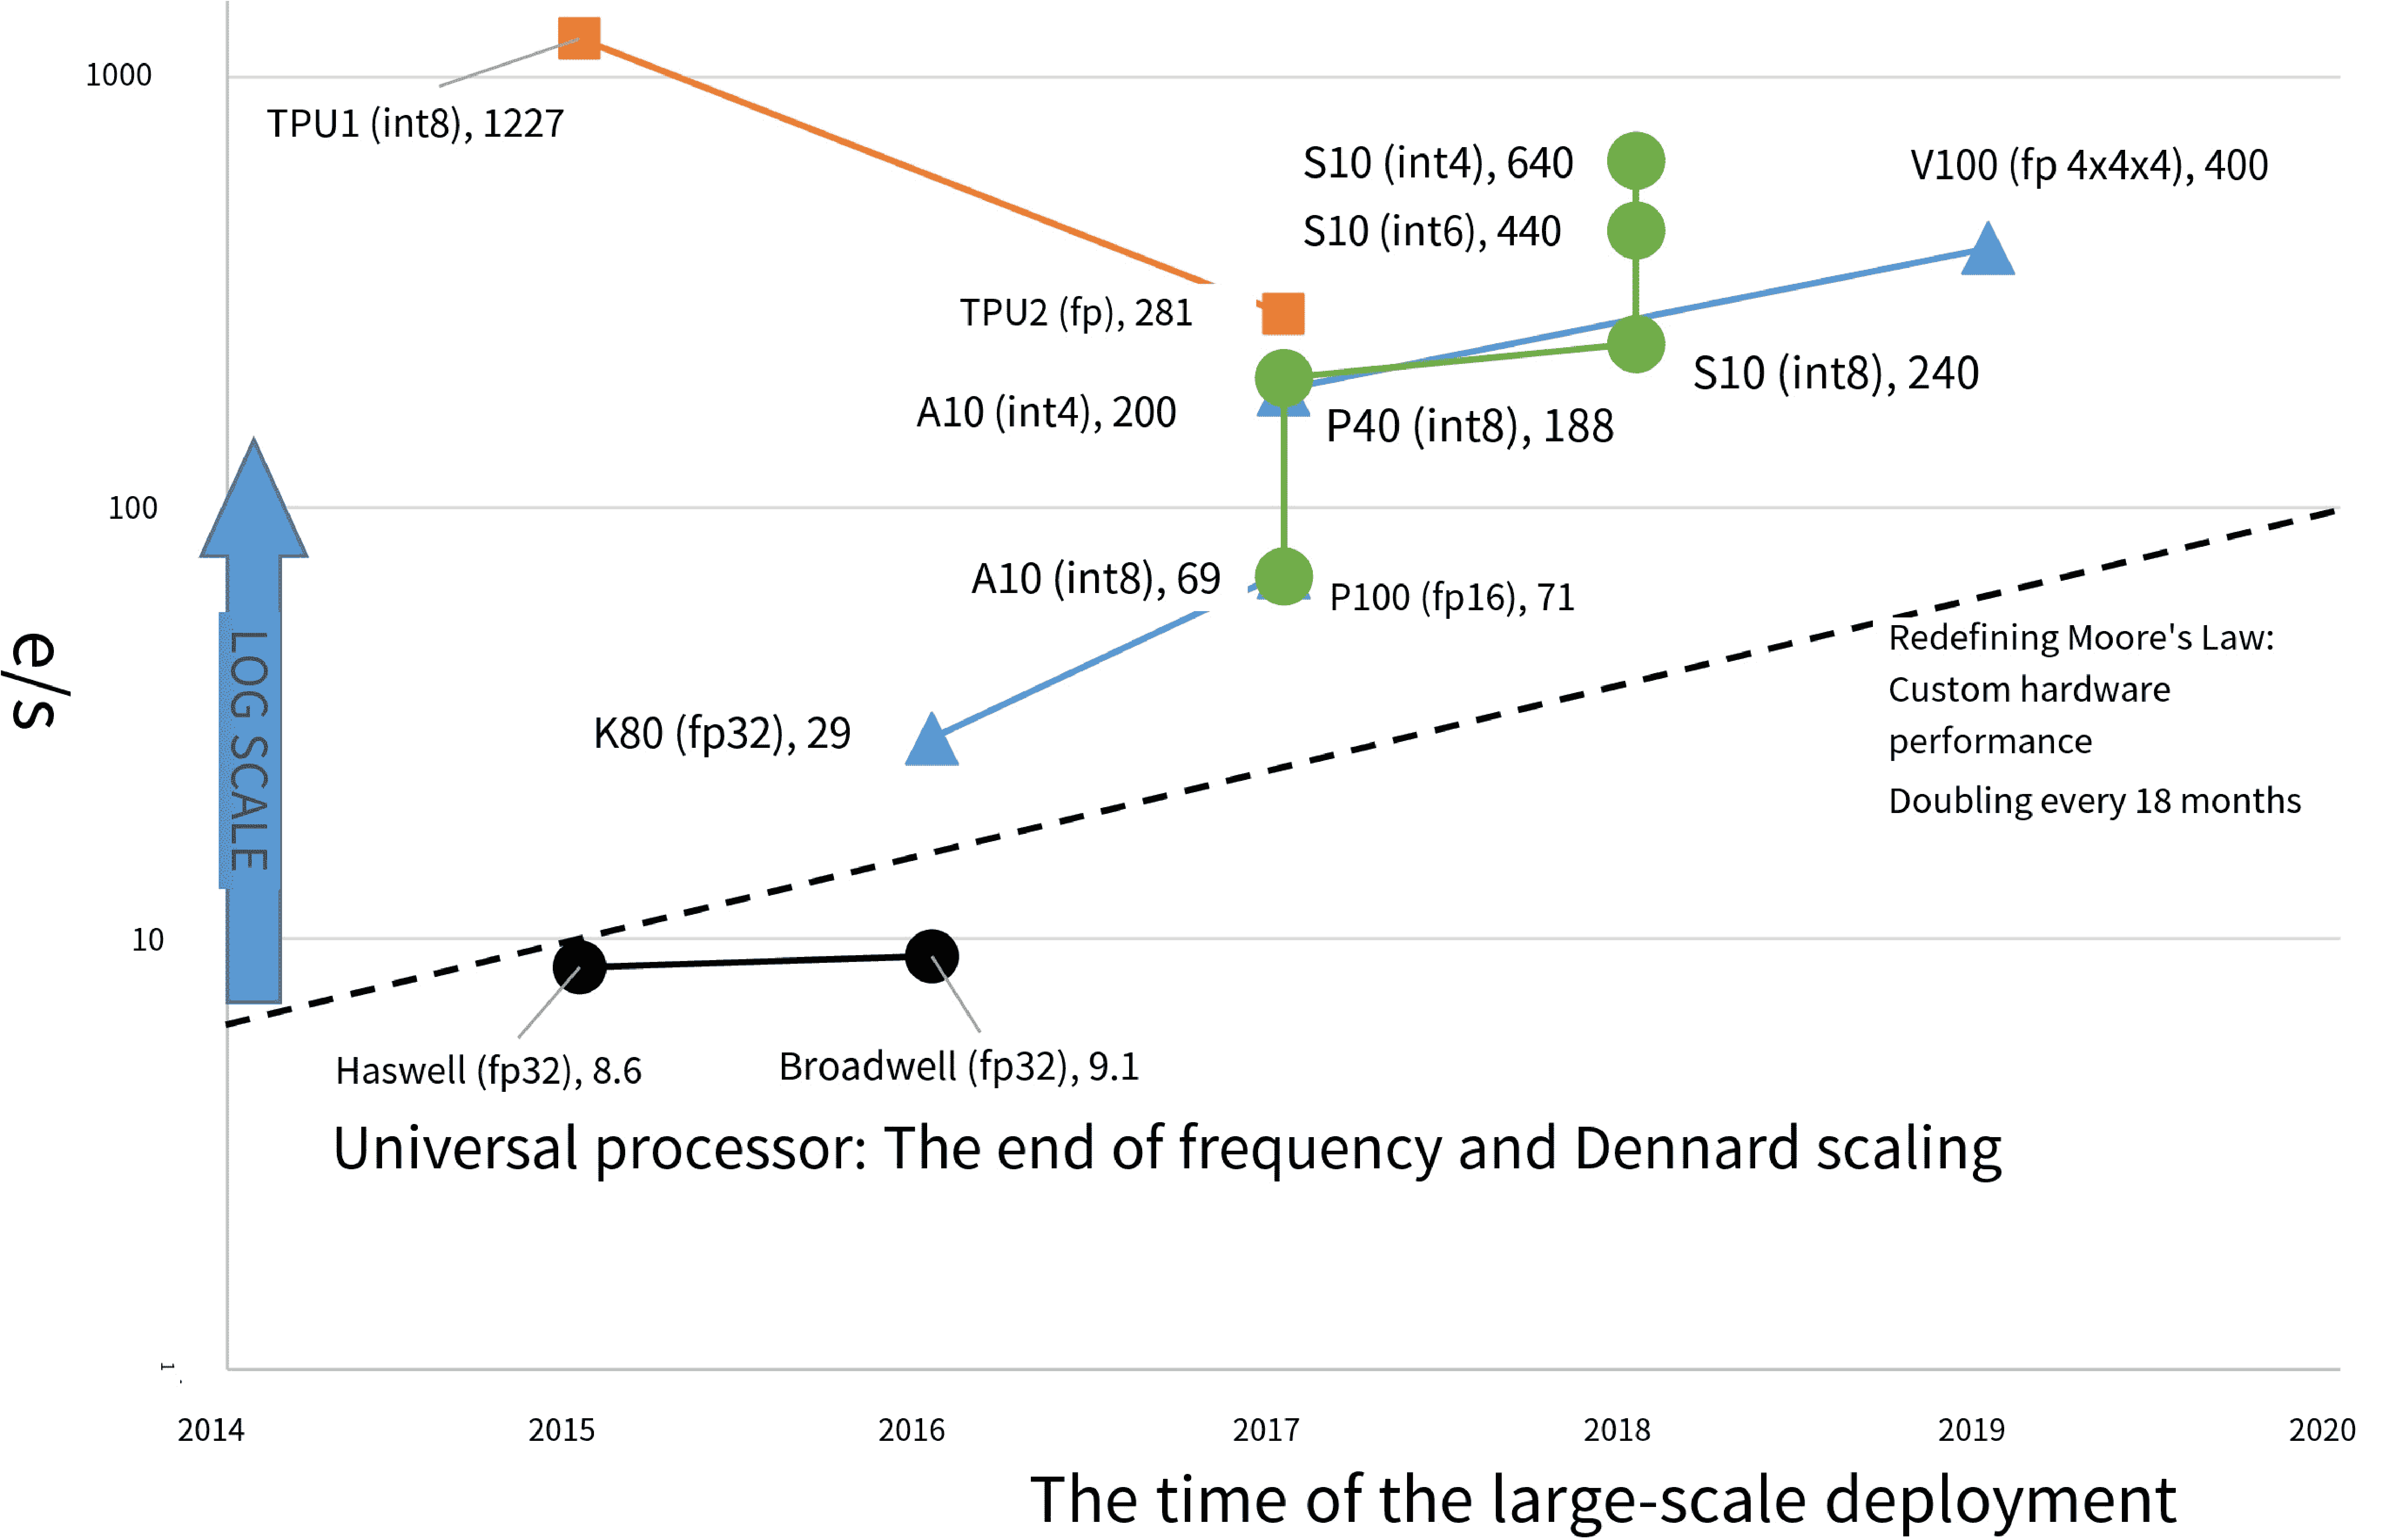
\includegraphics[width=0.8\textwidth]{figures/moores_law_redefined.pdf}
	\caption{通用处理器的频率和 Dennard 缩放逐渐终结,但定制化硬件重新定义并延续了摩尔定律。}
	\label{background:fig:moores_law_redefined}
\end{figure}


定制化硬件性能的快速提升主要来自两方面。一方面,由于较先进制程的一次性研发成本(NRE)很高,一个领域在从通用计算走向定制化计算的初期,定制化硬件使用较为落后、成本较低的制程,而随着该领域算力需求的提升和芯片设计经验的积累,逐渐使用更先进的制程。通用处理器由于多年的积累和巨大的产量,一直在使用几乎是最先进的制程。另一方面,定制化硬件的设计也在不断优化,也在与应用联合优化。以深度学习为例,很多模型可以通过降低参数精度、稀疏表达来减少运算量并保持预测精度。在图 \ref{background:fig:moores_law_redefined} 中,相同的 Arria 10 FPGA 芯片执行 4 位整数运算的能耗效率是 8 位的约 4 倍。


第二,操作系统的优化空间也是巨大的。上一节已经指出,网络、存储协议栈的大量开销作为 ``数据中心税'' 的重要部分,是值得优化的。

第三,现代软件享受着摩尔定律的红利,为了开发效率,一般使用高级语言模块化编程,而编译器对软件的优化并不充分。高级语言编写的现代软件,即使与多年前基于底层语言(如 C 语言)的软件功能相似,其性能往往也相差很多。``安迪-比尔定律'' \cite{langchaozhidian} 形象地刻画了这种现象,即高性能的新型处理器(以 Intel 的 CEO 安迪代表)所增加的性能,往往被软件(以微软的创始人比尔·盖茨代表)所消耗,最终用户感受到的性能仍然是相似的。从编程框架、编译器等角度优化软件的性能也有很大的空间。David Patterson 指出,把 Python 语言重写为 C 语言,应用程序的性能可以提高 50 倍,而如果使用一系列优化,实现 1000 倍于 Python 的性能提升并不是梦想 \cite{python-to-c}。本文的软硬件结合加速可以认为是这方面的尝试。把软件按照数据面和控制面进行划分后,性能敏感的数据面采用硬件加速,而控制面仍然用软件提供开发效率和灵活性。

第四,现代数据中心的资源利用率较低,有较大的优化空间。例如,数据中心内大部分物理服务器的平均使用率只有大约 10\% 到 15\%,但是闲置时的功耗却与使用率最高时相差仅 30\% \cite{barroso2018datacenter}。一方面,服务器和硬件的节能设计可以改进,以在使用率较低甚至闲置时尽量降低功耗。另一方面,云计算的一项优势就是支持热迁移,理论上可以在客户几乎不感知的情况下,根据虚拟机的计算、内存、存储、网络等需求,把需求互补的虚拟机打包安排在一台物理服务器主机上,从而最大化利用物理服务器的各种硬件资源。目前,由于种种技术限制,热迁移对客户服务会造成一段时间的性能下降甚至中断,因此在云计算中的利用还不够广泛。

在云计算平台中,软件和硬件的环境都由服务商控制,在达到了一定的规模以后,各种形式的定制化都成为可能。只要能够提高性能,降低价格,增强竞争力,云服务商有足够的动力去定制芯片,改变网络协议,改变服务器架构,更改操作系统,甚至重新编写应用程序。

综上,数据中心应用的需求、通用处理器的性能局限以及云计算规模化的趋势,使软硬件全栈优化成为数据中心的趋势。
系统性能优化不仅可以节约成本、满足客户对性能的需求,还可以简化系统架构,减少设计中的权衡。例如,在应用层延迟预算固定的情况下,如果虚拟化的开销减少了,就可以做更复杂的计算,达到更精确、实时性更强;如果远程过程调用的延迟降低到 1/3,一个应用层请求就可以调用 3 倍数量的远程过程调用,便于后端的微服务解耦。如果键值存储的性能足够高,就可以不在应用层加入额外的缓存,减少重造轮子,且避免缓存不一致的潜在问题。如果套接字通信原语的性能足够高,应用就不必修改来使用 RDMA 等较复杂的通信原语。

如果说以上现有系统的性能优化都是消极的动机的话,系统性能优化还有一种积极的动机,即提出高效抽象、赋能更多应用。
例如,高带宽、低延迟的 RDMA 网络使大规模深度学习和数据处理成为可能。在传统低速网络中,通信的开销可能高于分布式带来的收益。
固态存储(SSD)已经改变了存储和数据库系统的设计范式,使大数据的随机访问和实时处理成为可能;非易失性存储(NVM)将带来更大的改变。
从数据中心以外更大的范畴看,GPU 早期用于显示卡和图形计算加速,但近年来成为深度学习的主要算力支持;4G 移动网络因其相比早期移动网络带宽更大、单位流量成本更低,助力了移动互联网的快速发展。
数据中心基础架构研究者的最高使命就是提出普遍的抽象,使开发者可以在这些抽象的基础上可靠而高效的实现应用程序。
渴望提出这样的抽象,是数据中心性能优化工作无穷的毅力和耐心的源泉。

本文致力于用软硬件全栈优化的方法降低 ``数据中心税'',提高以虚拟化为代表的细粒度计算和大规模分布式系统的性能。下一节将介绍数据中心硬件的发展趋势,并引出本文所引入的数据中心新硬件:可编程网卡。


\iffalse

\subsection{芯片的发展}

计算机体系结构的进步是和半导体集成电路的发展分不开的。可以毫不夸张地说,计算机的发展是集成电路技术最大的推动力,也是最大的获益者。过去半个多世纪以来,集成电路一直大致保持着摩尔定律预测的速度发展,高度集成的芯片带来一次又一次计算机体系结构的革命,从巨型机(MainFrame)到个人电脑(Desktop),从服务器到云计算平台,从笔记本电脑到移动计算,集成电路使得各种形态的计算机快速地渗透到生活的方方面面。而另一方面,正是计算的需求,推动了中央处理器 (CPU),内存 (DRAM),图形加速器 (GPU) 以及高速网络芯片的发展。芯片技术和计算机体系结构相辅相成,共同推动了计算机系统软件和计算机应用的发展,使信息技术在短短的几十年中获得了如此重要的社会和经济地位。

目前信息科学技术依然处于一个高速发展的阶段,新的应用层出不穷:人工智能、物联网、虚拟现实、区块链,新兴的方向让人目不暇接,每一项技术都有无穷的潜力,可能推动人类社会进入全新的未来。而另一方面,基于半导体硅的CMOS集成电路芯片技术由于受到物理规律的限制,已经开始达到瓶颈。一方面芯片的线宽(Feature Size)在5纳米以下已经很难进一步缩小,而另一方面功耗和散热已经成为现代芯片技术难以绕过的难题。在这种情况下,计算机技术会何去何从?未来的计算机如何满足不断增长的计算能力的需求?

这篇短文探讨计算机系统在未来几年中发展的可能方向,尤其是集成电路技术如何与计算机体系结构继续相互推动,提高计算的速度和效率,满足不断增长的算力需求。目前学术界和工业界的共识是,科学家们看来不太可能找到短期内能代替CMOS的技术,计算机技术性能的提升在短期内必须主要依靠计算机体系结构的创新。这篇短文着重探讨一下云计算平台的体系结构可能的发展趋势和方向。在可以预见的未来,云计算会是非常重要的计算平台,它会提供人类社会主要的算力,推动整个世界的数据处理能力。当然,移动计算、物联网以及其它“端”也是非常重要的发展方向,但限于篇幅,这篇短文就不详细探讨这些方面的发展。

\subsection{云计算平台的变革}

在21世纪初期,云计算的概念刚刚起步的时候,云计算的平台基本上就是一个普通的企业数据中心,只不过规模比较大而已。当时的云计算与传统意义上科学计算用的超算平台在硬件上有很大区别。科学计算用的超级计算机往往使用定制的芯片,定制的网络,不惜成本地追求最高的性能。而云平台的特点就是把普通的低端商用服务器规模化,用软件实现高容错、高可靠性,降低成本,提供高性能的服务。

随着云计算商业模式得到用户的认可,特别是公有云的概念被广泛接受,经过近二十年的发展,目前主要的云计算平台提供商已经取得了巨大的商业成功。云计算平台的规模已经大大扩张。业界领先的云平台已经拥有遍布世界各地数以百计的数据中心以及数以百万计的服务器。这对计算机的体系结构带来了非常多新的挑战。建设一个大规模的云计算平台需要巨大的投资,任何能够减少单机成本的创新都能带来极高回报;云计算需要大量电力维持运转,提高系统的效率,降低功耗是重要的指标;云计算平台的一个大卖点就是弹性和灵活的配置,如何提供弹性同时尽可能减少系统空闲是一个复杂的问题;云计算需要保证可靠性,需要易于管理,需要保护私有信息,这里有非常多的挑战都需要解决。

在计算机发展的早期,软硬件是由同一个公司团队开发的,许多黑科技在这个大环境下被发明创造出来,对后世产生了深远影响。随着计算机的发展,设计分工变得越来越细,CPU、内存、网络、操作系统等等计算机的组成部分逐渐由各个专业公司独立完成,这使得工程师们必须遵守现有的体系框架,跨界创新变得非常困难。虽然在某些专用领域(例如游戏机)设计师们还可能做系统全盘考虑,但在通用计算领域这几乎成了不可能的任务。


\subsection{可编程逻辑阵列FPGA 和专用集成电路 ASIC}

为了更好了解集成电路和计算机体系结构,需要在这里简单介绍一下两个重要的集成电路技术。

ASIC(Application Specific Integrated Circuit,专用集成电路)是为某些应用专门开发的集成电路芯片。ASIC开发门槛比较高,研发周期也比较长。在目前的技术水平下,中等复杂度的ASIC前期投入的一次性开发成本(NRE, Non-Recurring Engineering)会在数百万到一两千万美元左右,并且需要一两年的开发周期。

FPGA(Field Programmable Gate Array,可编程门阵列)是一种可以重新定制 (reconfigurable) 的集成电路元器件。直观上来说,FPGA就是一个可以用编程的方法重新组合的一大堆电子元器件。这些元器件包括逻辑门(如与,或,非门),寄存器 (Register),加法器,静态内存(SRAM)等等,用户可以定制它们之间的连接从而组成不同的电路。如今的FPGA除了基本元件,还加入了越来越多的DSP和硬核(hard IP),以提高乘法、浮点运算和访问外围设备的性能。FPGA的优点是技术比较成熟,开发门槛相对其它集成电路(如ASIC)较低,部署后依然可以修改,缺点是性能比专用芯片差。

FPGA传统上被广泛应用于原型设计,逻辑电路模拟,以及高端路由器等等的领域。最近几年FPGA开始被在数据中心中得到越来越广泛的应用。在数据中心中,FPGA主要被用在两个方面,一方面是用于部署后依然可能需要改变的应用上,比如网卡。由于公有云的网卡上经常需要调整或添加协议,需要经常对硬件重新编程。另一种应用是计算加速:对于一些特殊的计算,可以利用FPGA可以高度并行化的的特性加速。在数据中心中用FPGA加速应用的一个大概的规则是10,100,1000规则:应用需要可以被加速十倍以上,如果加速比太小就不值得做硬件的实现了;被加速的部分核心大约相当于100行以下的代码,更复杂的逻辑用硬件实现难度就会比较大;而计算在数据中心应该需要至少1000台左右的服务器,如果服务器数目远远小于1000台,可能就不值得开发硬件方案了。当然,这些数字都是非常粗略的估计,应该根据FPGA的部署情况,应用本身的价值,以及开发人员的实际情况做相应调整。

在过去,开发ASIC往往是专业硬件芯片公司才能做到的事情。但随着云计算平台规模的不断扩大,云计算系统公司也开始尝试针对自己的云独立设计专用芯片。
\fi

\section{数据中心硬件的发展趋势}
\label{background:sec:hardware}



现代计算机系统大致可以被划分成四个主要部分:计算系统(Compute)、内存系统(Memory)、存储系统(Storage)以及网络和互连系统(Networking and Interconnect)。


\subsection{计算系统}

计算系统是整个计算机的核心,通常是由中央处理器CPU和一些为特殊应用服务的加速器构成。从整个计算机体系结构的发展来看,计算系统上的创新可能是最受关注的一个领域了。

在过去,计算系统基本上就等同于CPU,而CPU上的创新是由Intel、IBM等少数几个大公司主导的。传统上计算力是计算机系统中相对比较富裕的资源。一方面得益于摩尔定律及CPU体系结构的进步,CPU的速度和效率得到了长足的进步;另一方面其它的子系统例如硬盘,内存和网络因为相对缓慢的进展而往往成为实际应用的瓶颈。这种情况在最近几年发生了很大改变:随着新的硬件如固态硬盘和高速网络的出现,I/O往往不再是瓶颈;而新的应用如深度学习和内存数据库等对算力有极大需求,传统的CPU已经越来越难以支撑这些应用。正因为如此,在计算系统上创新,也就是大家通常所说的异构系统成为近年来计算机体系结构研究的一个热点。

\subsubsection{深度学习加速器}

最近深度学习的热潮,使得计算加速成为一个热点。从大学到工业界,从初创企业到业界巨头,从传统的半导体公司到传统的应用软件开发商都在尝试设计专门针对深度学习应用的硬件加速器,为小到低功耗的IoT设备,大到整个数据中心设计解决方案。在云计算领域,谷歌作为利用集成电路ASIC加速深度学习的先行者,为此设计的专用张量处理器(TPU)目前已经发展到第3代 \cite{tpu},无论从技术创新,吸引眼球,还是商业运作方面都取得了极大的成功。微软利用FPGA做深度神经网络(DNN)加速,也已经在Azure云平台上线 \cite{serving-dnns-real-time-datacenter-scale-project-brainwave,a-configurable-cloud-scale-dnn-processor-for-real-time-ai}。

深度学习包括训练和推理两种场景。训练所需的内存大、运算复杂,大多部署在云数据中心,NVIDIA的GPU具有巨大的生态系统优势,仅有第三代TPU、Graphcore \cite{graphcore} 等少数深度学习加速器正在挑战其垄断地位。推理的应用场景则较为异构。移动计算场景下低功耗是最重要的需求,如寒武纪神经网络处理器以知识产权(IP)授权的形式集成进入华为麒麟970移动处理器;搜索推荐、自动驾驶和虚拟现实场景下,既需要毫秒甚至微秒级的低延迟,又需要较高的吞吐量。推理的多种场景下不仅有不同的性能指标,所需的神经网络运算也不尽相同。加速器除了支持循环神经网络、卷积、矩阵乘法、正则化等经典神经网络运算,还需要与场景相关的算法共同演进,利用稀疏化(sparsity)\cite{yao2018balanced,cao2019efficient}、量化(quantization)等技术在不降低精度的前提下提高算力 \cite{zhang2015optimizing},并支持动态控制流等新兴的神经网络结构。

\subsubsection{FPGA和可重构硬件}

用FPGA做计算加速在学术界已经被研究多年,在某些特定的领域也得到了一些应用。而将FPGA大规模部署在通用服务器上却是最近几年才开始取得的突破。很多公司都开始做一些这方面的尝试,特别是微软和百度在有效利用FPGA做云计算加速方面做了很多工作。例如微软在Azure云平台上已经全面部署了FPGA模块 \cite{putnam2014reconfigurable,caulfield2016cloud}。百度将 FPGA 用于数据压缩 \cite{ouyang2010fpga}、数据库 SQL 处理 \cite{baidu-fpga-sql}、深度学习 \cite{ouyang2014sda} 和其他丰富的应用场景 \cite{ouyang2017xpu}。目前云厂商也将FPGA作为服务提供给第三方开发者。随着云端FPGA开发环境和开发工具的完善,越来越多的应用会利用FPGA的重构能力获得加速。

收购Altera后,Intel 推出了集成了FPGA的Xeon芯片,通过 UPI(即原来的 QPI)总线互连 FPGA 与 CPU,实现 CPU 和 FPGA 之间内存一致(coherent)的通信,这将大大提高 FPGA 作为 CPU 加速器的通信效率。而Xilinx则推出了全新的 Versal 可重构硬件构架 \cite{vissers2018keynote,vissers2019versal,gaide2019xilinx},将可重构硬件(FPGA),基于超长指令字(VLIW)的深度学习和传统机器学习加速器、数字信号处理器(DSP)和硬核(hard IP),以及多核通用处理器集成在一块芯片上,组成片上系统(System on Chip)。与传统 FPGA 相比,Versal 架构最大的区别是组成了片上系统,体现在三方面:第一,把内存控制器、PCIe 等外部接口的控制逻辑从可重构逻辑硬化成数字逻辑,减少了 FPGA 面积的开销,还能使 FPGA 实现即插即用。第二,认识到向量操作等大数据、机器学习常见计算在 FPGA 上实现的较低效率,并使用硬化的数字逻辑进行加速。第三,增加了通用处理器,可以处理复杂逻辑和控制平面,而无需绕回 CPU,这使得 Versal 片上系统可以直接驱动 Flash 存储等,组成低成本的存储服务器,而无需传统的 x86 CPU 等组件。片上系统的部件之间通过片上网络互连 \cite{swarbrick2019network,gaide2019xilinx}。Versal 架构针对数据中心服务器的多种应用加速,开发者可以把应用分解成通用处理器上的控制面、可重构硬件数据面、向量计算数据面,用合适的体系结构处理应用中的相应部分。这些技术必将对未来几年的云计算平台架构带来深远影响。除此之外,一些研究机构和初创企业开始再次尝试设计新一代粗粒度可重构硬件(CGRA)。粗粒度可重构硬件对于一些合适的应用可以兼顾FPGA可重构和ASIC高效率的优点,虽然过去的一些类似尝试最终没有取得商业成功,但云计算蓬勃发展的大环境很可能让这一技术焕发新的生命。
%对于面积越来越大的 FPGA,为了方便布局布线、加速编译和方便 FPGA 的空间复用,FPGA 厂商也从粗粒度可重构硬件中吸取一些设计,不再把 FPGA 的可重构片上资源(如 BRAM、DSP)集中在若干固定的位置,而是将 FPGA 划分成若干同构的区域,每个区域内都有相似的片上资源布局。


FPGA传统上被广泛应用于原型设计,逻辑电路模拟,以及高端路由器等等的领域。最近几年FPGA开始被在数据中心中得到越来越广泛的应用。在数据中心中,FPGA主要被用在两个方面,一方面是用于部署后依然可能需要改变的应用上,比如网卡。由于公有云的网卡上经常需要调整或添加协议,需要经常对硬件重新编程。另一种应用是计算加速:对于一些特殊的计算,可以利用FPGA可以高度并行化的的特性加速。在数据中心中用FPGA加速应用的一个大概的规则是10,100,1000规则:应用需要可以被加速十倍以上,如果加速比太小就不值得做硬件的实现了;被加速的部分核心大约相当于100行以下的代码,更复杂的逻辑用硬件实现难度就会比较大;而计算在数据中心应该需要至少1000台左右的服务器,如果服务器数目远远小于1000台,可能就不值得开发硬件方案了。当然,这些数字都是非常粗略的估计,应该根据FPGA的部署情况,应用本身的价值,以及开发人员的实际情况做相应调整。


\subsubsection{通用可编程加速器}

得益于深度学习的高速发展,传统的计算加速器比如NVIDIA的GPGPU以及Intel的Xeon Phi近年来也在数据中心和云平台上取得了很大的成功。除了深度学习,这些加速器还可以被用于加速科学计算,数据库检索,机器学习,图像处理等许多不同领域的应用。这些可编程通用加速器主要是利用计算的并行性来获得比CPU更高的性能和效率。但是,目前已有的这些加速器主要是为高性能计算设计的,除了 FPGA,还没有公司专门为云计算平台的一些主流应用比如数据压缩,网络包处理,加密解密等等设计一个通用的加速器。这很可能是一个有一定潜力值得挖掘的新方向。

对加速器来说,一大挑战是普通的内存无法满足并行计算需要的数据吞吐带宽。利用3D封装技术实现的HBM(High Bandwidth Memory)最近开始被广泛应用在这些加速器中。随着集成电路工艺的改进,集成计算和内存于同一芯片的PIM(Processing In Memory)方法开始重新受到重视,在这个技术上的突破可能给可编程加速器带来性能的飞跃。

\subsubsection{通用处理器}

在可以预见的未来,云计算中的大部分代码,特别是不易并行的代码,仍将主要在CPU上执行。为了隐藏访存延迟,提高流水线利用率,CPU使用乱序和推测执行来动态调度指令的执行顺序。过去的推测执行在微体系结构方面的副作用导致了 Spectre \cite{Kocher2018spectre}、Meltdown \cite{Lipp2018meltdown} 等安全漏洞,需要未来的CPU体系结构设计做出重大的改变。

乱序和推测执行受到指令窗口的限制,只能隐藏百纳秒级的延迟(基本对应于内存访问的延迟)。对于访问网络、存储、加速器等带来的微秒级延迟,还没有很好的解决方法 \cite{barroso2017attack}。简单地增大乱序执行指令窗口是不现实的,而操作系统现有的线程切换机制开销过高。编程语言现有的协程(coroutine)机制一方面使编程变得复杂,另一方面在访问网络、存储、加速器等外设时仍然依赖开销较高的内存屏障。未来计算机体系结构的一大挑战是解决对程序员透明的微秒级细粒度并发。这需要CPU体系结构、编程语言和操作系统的协同设计。

通用处理器并不仅仅只存在于服务器的中央处理器。加速器、硬盘、网卡等设备上一般也有用于控制和通信的处理器。此类处理器往往需要根据领域需求定制,而使用MIPS或ARM需要不菲的授权费。最近,加州大学伯克利分校提出了RISC-V \cite{asanovic2014instruction},一种开放的指令集架构(ISA),以缩短定制化处理器架构的周期和成本。RISC-V以及其相对应的软件生态的出现和完善使得Intel,ARM之外的公司和个人也可以在CPU体系结构上创新,而不用被编译器,操作系统,及上层的应用生态限制。RISC-V这一开放指令集架构的运动必然会对未来CPU的生态产生非常大的影响。很多公司会有机会完全抛弃Intel和ARM另起炉灶,为自己的应用设计和生产自己的CPU。

\subsubsection{软件的挑战}

对所有提高计算系统效率和性能的技术来说,可编程性永远是一个无法绕过的坎。近年来,硬件的高层次综合技术和软件并行编程技术都有了很大的进展,这降低了利用新的计算资源的门槛。尽管如此,如何方便而有效地利用这些非传统的计算资源依然是一个长期的难题,需要大量的持续投入。

不同于PC时代分工明确、由各个公司分别掌控的标准化模块,云计算中从硬件到软件全栈优化和定制化的需求是开源生态系统近十年来蓬勃发展的主要驱动力之一。未来的异构计算软件框架也将形成开放的软硬件接口标准和开源生态系统。

\subsection{内存系统}

内存系统用来存放程序运行时的代码和数据。目前几乎所有的计算机系统上,内存系统都是由少量基于静态内存(SRAM)的缓存(Cache)和大量的动态内存(DRAM)组成的。除了极少数为科学计算或超大型数据库设计的高性能计算机外,绝大部分计算机上的内存只能被本地同一主板上的一颗到几颗CPU芯片访问。在过去的半个世纪以来,内存系统的主要特性都一直没有什么变化,非常令人振奋的是,最近几年内出现的几项新技术可能会改变这一现状。

\subsubsection{高速非易失性内存(Non Volatile Memory,NVM)}

目前被广泛使用的动态内存(DRAM)制造工艺已经接近物理极限,价格一直居高不下,另外,DRAM需要不断刷新来保持数据,功耗较高。长期以来科学家们一直在寻找能够代替DRAM的存储器件。通过科学家们多年以来不懈努力,一直声称有希望取代DRAM的高速非易失性内存目前看来终于快要进入实际应用阶段了。相比传统的NAND Flash,新一代的高速非易失性内存存取速度要快得多。虽然它们短期内还不能完全取代DRAM,但至少希望能够在不久的将来会代替一部分普通内存。目前看来,Intel和Micron合作的3D XPoint技术 \cite{3d-xpoint} 会是最快进入市场的非易失性内存,另外一些基于忆阻器件(ReRAM) \cite{akinaga2010resistive} 和磁阻器件(MRAM) \cite{tehrani1999progress} 的非易失性内存可能会紧随其后进入市场,学术界也在积极研究相变内存(PCM) \cite{raoux2008phase,lee2010phase} 和 STTRAM \cite{kultursay2013evaluating,apalkov2013spin} 等非易失性内存技术。

非易失性内存相比DRAM有价格低,容量大,功耗小,断电可以保持数据的优点,但同时又有存取速度慢,写入周期有限等等限制。如何有效地利用非易失性内存目前是一个重要研究方向。
目前,大多数工作把非易失性内存当作介于动态内存和闪存持久化存储之间的存储层级,即所谓的 ``慢速内存'',形成两层的异构主存体系结构 \cite{dulloor2016data,agarwal2017thermostat}。
在应用程序的使用接口方面,大多数工作把非易失性内存抽象成块设备 \cite{bailey2011operating,huang2014nvram,kim2016nvwal,mogul2009operating,nanavati2017decibel,hu2017log} 或文件系统 \cite{condit2009better,yang2015nv,xu2016nova},并支持标准的 POSIX 接口。
为了降低操作系统软件存储协议栈开销,NVTree \cite{yang2015nv}、NVWal \cite{kim2016nvwal}、NOVA \cite{xu2016nova}、Decibel \cite{nanavati2017decibel}、LSNVMM \cite{hu2017log} 等工作旨在高效管理存储在非易失主存中的数据。
PASTE \cite{honda2018paste} 提出了存储和网络协议栈的协同处理。
从体系结构的角度,为了消除应用程序访问非易失性内存的额外软件开销,AMD 等 CPU 厂商正在通过改进内存控制器,把非易失性内存映射到 CPU 的内存地址空间,从而应用程序可以像访问动态内存那样访问非易失性内存。


\subsubsection{内存解聚(Memory Disaggregation)}

传统的服务器上的CPU、内存、存储等资源聚合在一起成为独立的单元,一台服务器需要通过网络API访问远程的资源,使用上非常不便和低效。目前一个计算机体系结构研究的热点是资源解聚(Resource Disaggregation),也就是让资源可以不受服务器物理边界的限制被透明地远程访问。内存解聚(Memory Disaggregation) \cite{lim2009disaggregated,han2013network} 指的是计算机的计算系统(CPU、GPU等)可以自由而透明地高效共享远程计算机的内存,这样可以大大增加内存的利用率,降低云计算平台的成本。

要想实现这一目标,计算机系统的软硬件都需要做很大的改变。从硬件上来看,如何能让远程访问满足内存所需的带宽和延迟要求是一个巨大挑战。幸运的是,利用内存访问的局部性,如果一部分热数据仍在本地,剩余的数据通过远程访问,则远程内存的带宽和延迟要求能比本地内存大大降低。加州大学伯克利分校的研究 \cite{gao2016network} 指出,要把内存解聚后的系统性能与全部使用本地内存的差距控制在5\%以内,带宽需要达到40 Gbps,端到端往返延迟需要不超过3至5微秒。现代数据中心的带宽已能满足大多数应用的需求,但延迟仍有一个数量级的差距。本文提出的软硬件结合全栈优化将有助于网络延迟达到上述需求。

从系统软件上来说,如何有效共享远程的内存,让应用克服远程内存访问的延迟和带宽限制也有很多问题需要解决。与传统的交换空间(swap)不同,把一块内存放在远程会减少对应远程机器的本地内存,因此一块内存放在本地还是远程、放在远程的哪台机器上,需要根据集群全局的信息来决策 \cite{gu2017efficient}。另外,远程内存的延迟远大于本地内存,当等待远程内存时,如果不希望CPU核闲置,就需要调度其他任务。这种微秒级的延迟隐藏仍是一个没有很好解决的问题 \cite{barroso2017attack}。

\subsubsection{HBM(High Bandwidth Memory )}

HBM使用2.5D集成电路封装技术,将内存和逻辑芯片封装在同一硅片衬底中,从而提供更高的带宽。前面已经提到HBM已经开始被用到计算加速器上,但目前这一技术还没有用在通用的计算CPU上。一方面普通外置DRAM已经可以满足通用CPU带宽的需求,不需要高成本的HBM,另一方面现代应用通常需要很大的内存容量,目前的HBM还无法满足。但是从系统整体设计的角度来看,计算加速器独占高速内存是不正确的设计。CPU应该和加速器共享高速内存,这样不仅能够更充分地利用HBM,同时CPU和加速器之间的协同也更加简单高效。但是目前由于CPU和加速器是由不同公司设计制造的,所以只能采用一个权宜的设计。如果单个公司控制整个系统的设计,可能结果就不一样了。在微软的 XBOX One X 中,CPU就是和GPU共享高速的GDDR5的,而AMD的APU也一直在推动CPU和GPU共享内存。随着计算加速的普及,在以后的云平台中CPU可能会与加速芯片共享HBM。从CPU角度看HBM就是一块高速内存,而普通DRAM就会成为一个容量的扩展,变成内存层次(Memory Hierarchy)中的另外一层。

\subsubsection{软件的挑战}

传统的内存层次(Memory Hierarchy)通常有三层。cache是透明的,用户的程序一般不需要直接操作;而可以按照字节寻址的DRAM的性能是统一的,这是应用程序需要控制的内存区域;对用户完全透明的虚拟内存(Page Swap)虽然理论上非常优美,但由于内存与磁盘之间的延迟相差多个数量级,实际使用中很小比例的内存不命中就会极大影响应用的性能,所以一般是万不得已的最后选择。新一代的内存系统势必需要在传统的内存层次中再增加一个层次。用户程序是需要显式调用专用的API去存取这片内存,还是应该对应用透明?这个层次的内存应该如何能够被高效使用目前还没有定论。

\subsection{存储系统}

存储系统过去主要是由基于磁介质的硬盘和磁带组成,近年来基于NAND lash的固态硬盘被广泛应用于数据中心,而磁带已经开始淡出历史舞台。与内存系统不同,存储系统主要用来存放需要长期保存的数据。

\subsubsection{SCM(Storage Class Memory)}

SCM实际上是上一小节中讨论过的高速非易失性内存的另一种描述方式。在传统的计算机体系结构中,基于DRAM的内存和基于硬盘的存储是完全不同的两个系统,它们分别由操作系统中的内存管理系统和文件系统分别管理,基本上井水不犯河水。可是随着技术的发展,高速非易失性内存有潜力成为可以同时代替内存以及硬盘的一种器件,这时文件系统和内存系统的边界就开始模糊起来了。将高速非易失性内存用文件系统管理起来,利用它的非易失特性储存需要长期保存的数据就是SCM。SCM的出现对存储系统提出了新的挑战,如何有效地利用SCM高带宽、低延迟、可字节寻址的特性加速应用程序是一个需要解决的问题。

首先,机械硬盘和基于NAND Flash的固态硬盘是以 ``块''(block)为基本单位来读写的,从而随机读写的性能远低于连续读写。SCM可以按照字节寻址和读写,随机与连续读写的性能差距较小,从而降低了应用对数据排布的要求。很多应用可以把SCM文件映射到内存后直接访问,省去在文件存储格式和内存数据结构间来回转换的开销。

其次,传统系统为了在断电或系统崩溃后能够恢复,往往需要日志和快照技术来把一致的内存状态显式写入存储系统。利用SCM的非易失特性,把DRAM作为SCM的写通(write-through)缓存,应用就可以直接操作其上的数据结构而无需额外的日志和快照。

\subsubsection{存储解聚(Storage Disaggregation)}

类似于内存解聚,存储系统同样可以通过解聚来提高利用效率和性能。微软研究院将存储系统的解聚分为四个层次 \cite{legtchenko2017understanding}。一是配置解聚,即标准的机柜(rack)离线配置成存储阵列或计算阵列。二是故障解聚,即计算节点发生故障时把其硬盘分配给新的计算节点,无需搬运数据即可恢复服务。三是动态弹性解聚,即根据计算和存储的需求比例动态调整每块硬盘属于哪个服务器。前三个层次中,每块硬盘在每个时刻只属于一个服务器。四是完全解聚,即每个服务器都可以访问任意设备上的任意文件,还可以在IO操作的细粒度上做负载均衡,当然这对IO控制器的负载要求较高。

与内存系统相比,由于存储系统本身的带宽较低、延迟较高,存储系统解聚面临的挑战相对要小一些,一个主要的问题是如何能在资源共享的情况下能够减少用户之间的相互干扰(即性能隔离)以及保证服务的质量(QoS)。

\subsubsection{开放通道(Open Channel)SSD}

如今服务器里的固态硬盘大多基于NAND Flash。NAND Flash的每个闪存块需要先擦除再写入,每次擦除会造成一定的磨损,多次写入有的闪存块就会损坏;闪存块读取次数多了、闲置时间长了,上面的数据也会流失。因此,固态硬盘中的闪存转换层(FTL)除了从逻辑地址到物理地址的映射,还需要做一系列的处理。这些处理需要预留一部分存储空间、占用带宽来做垃圾回收和冗余,还会导致写操作时搬运周围数据带来额外开销。如果考虑到应用的读写特性和数据中心的外部冗余,FTL的很多操作在云计算数据中心中是不必要的。因此,百度 \cite{ouyang2013active} 提出绕过 FTL 层,由应用程序直接管理闪存阵列,FTL 的功能与应用程序就可以协同设计以提升性能。这种由主机软件实现 FTL 层的 SSD 被称为开放通道(Open Channel)SSD,近年来在越来越多的数据中心流行。

\subsubsection{软件的挑战}

传统存储系统操作通常需要操作系统的参与。过去,硬盘的速度较慢,操作系统的开销往往可以忽略不计。随着高性能存储介质的出现,应用程序与操作系统之间的上下文切换以及操作系统内文件系统和块设备层的开销逐渐成为性能瓶颈。为此,Intel 提出的SPDK \cite{spdk} 提供了绕过内核的应用直接访问存储接口。然而,当多个应用需要共享文件系统时,应用间的权限管理、并发控制和QoS仍是有待研究的问题。

\subsection{网络和互连系统}

网络(Networking)系统通常指用来连接多个计算机使它们之间能够相互通信的系统,而互连(Interconnect)一般指计算机内部的部件之间的连接。通常情况下这两种连接是有着巨大差别的,属于两个完全不同的学术领域。一个典型的网络,比如数据中心网络,通常需要跨越较长距离、对延迟不敏感的传输,需要多层路由和交换来连接为数众多的节点,丢包是靠软件检测和恢复的,且一个组件的故障一般不会影响网络其他部分的正常运行;而一个典型的互连,比如连接内存和CPU的总线,位宽和带宽会比较大,延迟很低,丢包会由硬件检测和恢复,但一个组件的故障可能导致整个系统的崩溃。

在互联网发展的早期,以搜索引擎为代表的应用比较容易并行化,因此对网络通信的需求不是很高,数据中心通常使用现成(off-the-shelf)的服务器通过以太网互连。最近,大数据处理、分布式机器学习、内存和存储等资源的解聚需要数据中心主机间低延迟、高带宽的通信。GPU和深度学习处理器为了做分布式训练和推理,也需要建立可扩放(scalable)的互连。由于高速可扩放通信需求的推动,有一个很有意思的趋势就是融合传统的网络和元器件之间的互连。比如常见的PCI-Express,开始设计的时候是为了连接单一机器内的不同部件,但是现在,PCI-E也被设计为可以交换的一个协议;而以太网的开始时是设计为连接局域网内计算机的一个网络,而如今一些器件间的连接也开始使用以太网的连接方式。

\subsubsection{低延迟无丢包的可扩放互连}

理想的网络和互连需要既能扩放到数据中心内数以百万计的设备和组件,又有低延迟、高带宽、无丢包的特性,还能容忍部分组件的故障甚至恶意攻击。为此,网络和互连的设计者一方面可以从很多历史设计中吸取经验,如超级计算机、片上网络、核心路由器的线卡间互连、电路交换网络、时分复用网络等;另一方面可以利用新的物理层技术,如光交换芯片、激光通信和60G无线网络等。

数据中心内从发送端网卡到接收端网卡的网络延迟主要包括光纤上的传播延迟、交换机的处理延迟和交换机内的排队延迟,其中排队延迟占了主要部分。为了降低排队延迟,数据中心交换机普遍使用ECN、RED等机制来把拥塞情况反馈给发送端,但这个反馈延迟往往较长,且不能消除来自不同发送端的数据包恰好撞在一起导致的偶发排队。为此,近期一系列研究在重新思考现有的拥塞控制算法,交换机也需要更灵活的动态控制来尽可能降低队列长度、保证服务质量。例如,微软 Azure 云 \cite{guo2016rdma}、阿里云 \cite{aliyun-rdma} 和华为云 \cite{huawei-lossless} 建成了大规模数据中心 RDMA 网络,构建了低延迟、高吞吐量、无丢包的数据中心网络,为大数据处理和大规模机器学习提供了高性能网络互连。

更深层的问题是Internet的端到端原则简化了设计、提高了鲁棒性,但也缩小了很多全局优化的空间。在端到端原则的指导下,很多数据中心的网络交换机和主机网络协议栈是由不同部门独立运维的,这也增加了协同设计的沟通成本。在网络和互连融合的未来数据中心,端到端原则在多大的范围内适用是一个值得思考的问题。

随着主机内异构计算和存储设备数量的增加,CPU的PCIe接口数量不足,PCIe交换机开始被引入主机;由于PCIe的带宽不能满足需求,GPU之间采用NVLink互连,随着互连GPU数量的增加也出现了交换机。数据中心网络的发展历史表明,异构计算设备之间的可扩放互连必须考虑容错性和安全性。为了解决计算和内存设备之间的互连,除了目前常用的 JEDEC DDR 和 PCIe 总线标准,工业界还成立了CCIX、Gen-Z和OpenCAPI三个开放标准组织,以及 Intel 的 IAL 和 RSD 两个总线标准。表 \ref{background:tab:ccix-pcie} 总结了这些总线标准的适用范围和主要支持公司。

\begin{table}[htbp]
	\centering
	\caption{总线标准的适用范围和主要支持公司}
	\scalebox{0.9}{
	\begin{tabular}{l|p{.5\textwidth}|p{.3\textwidth}}
		\hline
		总线 & 适用范围 & 主要支持公司 \\
		\hline
		\hline
		PCIe & 节点内 CPU、计算加速器、存储和网络间的互访 & 目前的事实标准 \\
		\hline
		DDR & 节点内 CPU 访问内存 & 目前的事实标准 \\
		\hline
		CCIX & 节点内 CPU 与内存一致(coherent)的计算加速器、非易失性内存间的互访 & AMD,ARM,Xilinx,Mellanox,Qualcomm 等 \\
		\hline
		OpenCAPI & 节点内 CPU 与内存一致(coherent)的计算加速器、非易失性内存间的互访 & Google,NVIDIA,Rackscale,IBM 等 \\
		\hline
		IAL & 节点内 CPU 与内存一致(coherent)的计算加速器、非易失性内存间的互访 & Intel 私有协议 \\
		\hline
		RSD & 机架范围内的节点间互连 & Intel 私有协议 \\
		\hline
		Gen-Z & 机架范围内的节点间互连,以及节点内 CPU 访问内存 & AMD,HP,Dell,华为等 \\
		\hline
	\end{tabular}
	}
	\label{background:tab:ccix-pcie}
\end{table}

\subsubsection{可编程交换机}

可编程交换机是由需求和硬件两方面的趋势所驱动的。从需求方面来讲,网络的自动运维(self-driving network)变得越来越重要。要实现自动化的网络故障检测、诊断和恢复,就必须在网络中加入智能,而不能把网络看成一个黑盒子。为此,交换机中需要加入可编程的抓包和统计功能。不仅如此,利用交换机的高速数据包处理能力,可以加速分布式系统中的缓存、聚合、同步、事务处理等,而低延迟无丢包网络也需要可编程交换机硬件的支持。很多人认为在交换机中增加可编程性会增加芯片面积和功耗,其实并不尽然。Barefoot 公司指出,交换机芯片中约有30\%的面积用于串行IO通信,50\%的面积用于存储查找表和数据包缓冲的内存,只有20\%的面积用于数据包处理逻辑。随着交换机的带宽不断增长,芯片面积也在增加,此时用于数据包处理的20\%面积就有空闲,可以放入更多逻辑 \cite{barefoot-programmable}。

可编程交换机按照可编程性从低到高,可分为三个层次。一是符合OpenFlow标准的交换机,数据包处理逻辑是一条由若干个匹配-执行表串接而成的流水线,但每个表的匹配和执行都有一定的限制;二是符合P4标准的交换机,在流水线结构的基础上,每个表项的匹配规则、所执行的操作和数据包头的解析规则都可以定制;三是网络处理器,即使用为网络处理特别设计的众核CPU处理每个数据包,可以达到最大的灵活性,但单条网络连接的吞吐量受限于CPU频率。事实上,固定功能流水线、通用可编程流水线和网络处理器并不是泾渭分明的,在数据中心交换机中已经可以看到逐渐融合的趋势,例如采用交叉开关或片上网络来灵活互连各个数据包处理模块和片上内存。

为了简化交换机运维和管理,微软发起了SONiC白盒交换机开源项目 \cite{sonic}。首先,定义了一组交换机芯片API,交换机的硬件和软件就可以独立演进而无需担心兼容性问题。其次,设计了基于容器的模块化交换机软件架构,通过把持久状态独立于容器存储,实现了细粒度的故障恢复和零服务中断时间的在线升级。最后,提供了监控和诊断能力,以支持网络的自动运维。

\subsubsection{可编程网卡}

传统以太网网卡的功能相对简单,网络协议栈在操作系统内核里实现,软件中间件又给应用程序提供了RPC、消息队列等更高层的抽象。在云计算场景下,还需要虚拟交换机软件来实现网络虚拟化和防火墙等网络功能。因此,数据中心网络的端到端往返延迟平均情况就高达上百微秒,极端情况甚至可达毫秒级,远远不能满足低延迟分布式计算的需求。其中,软件的延迟占了主要部分。高性能计算中常用的Infiniband \cite{infiniband2000infiniband} 网络把大部分网络协议栈实现在网卡里,可以实现端到端微秒级的延迟,因此其中的远程直接内存访问(RDMA)技术开始在数据中心中流行。为了与现有数据中心网络兼容,数据中心的RDMA网卡通常使用以太网和UDP/IP,再在其上封装RDMA可靠传输协议。但云计算数据中心的RDMA部署比高性能计算复杂很多:首先,数据中心的规模大于高性能计算集群;共享同一物理主机的虚拟机需要隔离和QoS,也就是网络虚拟化;虚拟机需要热迁移和故障恢复能力;另外,数据中心应用种类繁多、通信模式复杂,需要套接字兼容性和 RPC 等高层抽象。
为解决网络虚拟化需求,很多云数据中心大规模部署了可编程网卡,以把软件中的网络功能卸载到网卡硬件。可编程网卡是本文讨论的重点,将在第 \ref{smartnic-architecture} 节中详细讨论。

\subsubsection{设备间的智能互连}

传统计算机架构中CPU是中心,所有外设之间的通信都要通过CPU。近年来,CPU性能的提升放缓了,GPU、FPGA、TPU等异构计算设备和网络、存储的性能却突飞猛进,因此CPU日渐成为瓶颈。网卡、GPU、NVMe SSD等设备迫切需要绕过CPU的直接互连互通,因此出现了NVLink \cite{foley2017ultra} 这样的专用互连,以及GPU-Direct \cite{gpu-direct} 和 NVMe Over Fabrics \cite{minturn2015nvm} 等直接访问远程主机设备的技术。Broadcom也推出了可以通过以太网连接的PCIe交换机,使PCIe跨越了主机的边界 \cite{broadcom-expressfabric}。

然而,现有的技术大多只能互连一定范围内的特定设备。为了让数据中心内的所有异构计算和存储设备都能跨越主机的边界直接互连,微软研究院提出了Terminus项目 \cite{direct-universal-access-making-data-center-resources-available-to-fpga},将互连(Fabric)作为一台服务器的控制中心,Fabric 控制器之间通过数据中心网络互连。通过在Fabric中加入智能,可以在不同厂商的计算和存储设备之间做 ``翻译'',使它们在统一的命名空间中能够互相通信;Terminus也可以实现不同设备间的访问控制、通信性能隔离和服务质量保证;另外,Terminus可以支持资源虚拟化,既可以把多个物理的计算或存储资源虚拟成一个对用户透明的逻辑资源,又可以把一个物理资源虚拟成多个逻辑资源来实现多个用户间的资源共享;最后,Terminus 上的FPGA和可编程的数据中心网络可以在数据传输过程中进行一些处理,加速一系列的计算任务。Terminus项目目前使用FPGA作为原型,在未来也可以实现为智能的PCIe交换机。它与智能网卡、智能交换机一道,构建起数据中心的智能互连(Intelligent Fabric)。此时的数据中心可以被真正看作一台大型计算机,CPU、GPU等异构的计算资源和SSD、SCM等存储资源通过智能互连相连接,把分布式系统的通信、调度、容错等机制隐藏在统一的抽象之下,给用户提供取之不尽的计算资源和前所未有的编程便利。


\subsubsection{软件的挑战}

与存储系统类似,网络系统传统上被视为慢速的外设,再加上交换机排队、网络协议栈和中间件的高延迟,目前很多分布式系统并没有充分利用数据中心网络的高带宽和低延迟。近年来,绕过内核访问网络的用户态协议栈如雨后春笋般出现,\textbf{改进多核调度的工作(如 Adam Belay OSDI 18), FIXME}。打破主机边界的软硬件协同设计将是网络和互连的趋势。

\subsection{全栈创新}

把整个世界看作一台大型计算机是微软CEO萨蒂亚·纳德拉的愿景,也是很多系统研究者的梦想。云计算的成功使数据中心吸纳了人类世界大部分的计算和存储,而数据中心可以看作是由计算、内存、存储和网络及互连四部分组成的一台大型计算机。系统就是从全局的角度考虑各种软硬件组件如何高效而可靠地协同工作,以及给用户提供怎样的抽象。从大型机、PC、传统数据中心到云计算数据中心,每个时代的系统结构都随着应用的需求而变化。

在目前机架服务器构成的数据中心中,一台标准(非深度学习)机架服务器的热设计功耗(TDP)为 300 至 500 瓦,按照目前的芯片制程,能够支持约 1000 平方毫米的芯片面积。
理论上可以量化计算各种应用负载在不同体系结构上的功耗性能比,进而在不同的芯片间分配这 1000 平方毫米,求得每种体系结构芯片的最佳面积。
然而,这种方法并不现实,因为在设计服务器系统时,必须考虑多方面的限制。
例如通用处理器 CPU 上需要运行客户基于 x86 的应用,而 Intel 和 AMD 可选择的 CPU 型号是有限的。
再如,一款神经网络处理加速芯片(NPU)从设计到量产至少需要一到两年时间,很难为了设计一款新服务器机型等待如此长的时间,而只能在市场上已经或即将量产的加速芯片中做出选择。
此外,芯片之间的互连也需要遵循一定的标准,如 PCIe、CCIX 等,一种新的互连标准尽管设计起来不难,但需要较长的时间来寻求芯片厂商的支持。很多时候互连标准的选择不是纯技术的问题。
最后,服务器机箱(chassis)的设计涉及到散热等问题,需要积累经验,而在已有机箱布局和散热设计的限制下,芯片和板卡的数量甚至功耗就受到一定的约束。
因为芯片、互连和服务器机箱的可选方案是离散的,需要对各种组合进行全面的比较和分析,并得出最佳的方案。
当然,随着应用负载的变化,云服务商和板卡、芯片厂商也会调整芯片的体系结构设计和互连标准,逐渐向理论上最优的服务器组件结构靠拢。

如果可以抛开由机架服务器构建大型数据中心的现有模式,就有更多全栈创新的可能性。

\iffalse
\subsubsection{深度学习加速器集群}

数据中心内的深度学习和传统机器学习需要处理海量的算力,单个芯片的性能不能满足需求。当多个芯片互联用于解决深度学习负载时,
\fi

\subsubsection{机架级计算(Rack Level Computing)}

目前的数据中心的基本组件是由固定数量的CPU、GPU、内存、存储等资源构成的服务器。一方面,一台服务器中能容纳的硬件资源数量较少,只能同时运行少量任务,每个任务对不同种类资源的需求不均衡,这就会导致服务器中有的资源短缺,有的资源闲置。另一方面,CPU、内存和存储技术在成本、性能和功耗方面的演进趋势大不相同,要增加一种新硬件,往往需要重新设计服务器主板和机箱,需要较高的成本和较长的上市周期。前文提到的内存解聚和存储解聚通过访问远程内存和存储,只能解决第一个问题,可以认为是资源解聚的一个过渡期方案。完全的资源解聚需要重新思考以服务器为中心的数据中心设计。目前的趋势是把数据中心的基本组件从服务器变成机柜(rack)。机柜由若干个资源刀片(resource blade)和高速互连组成,每个资源刀片是一个装满同一种硬件资源的物理容器 \cite{camcubeos}。这样,CPU、GPU、内存、存储等不同种类的计算资源分别装在不同的资源刀片里,可以独立演进。目前的存储阵列已经使用了类似机架级计算的架构,来实现存储介质容量与存储功能的独立演进 \cite{pelican}。当然,GPU和CPU仍然有本地DRAM或HBM内存作为缓存,而内存刀片则由高达数TB的DRAM或NVM组成,可以存储相对冷的数据。机架级计算的核心挑战是高吞吐量、低延迟的网络互连,这需要网络的物理链路、拓扑结构和传输协议的协同创新 \cite{r2c2}。

\subsubsection{边缘数据中心}

目前的云计算数据中心大多规模庞大,部署在电力成本低、网络条件好的地区。用户访问最近的数据中心,也往往需要数毫秒到数十毫秒的延迟,带宽也受到一定限制。随着物联网、机器视觉、虚拟现实、自动驾驶等技术的发展,终端数据产生了越来越多需要实时处理的数据,此时把数据全部上传到云端在带宽和延迟上都是不可行的。为此,边缘数据中心开始兴起,把云计算搬到距离用户更近的位置 \cite{edge-data-center},10 年前学术界提出的边缘计算终于成为现实的趋势 \cite{satyanarayanan2009case}。一方面,边缘数据中心可以降低用户访问互联网服务的延迟,例如现在的内容分发网络(CDN)服务。另一方面,边缘数据中心可以把终端设备上的部分计算和存储卸载到云端,降低移动设备的功耗、体积和成本,方便应用的部署和更新。

边缘数据中心将给云计算带来前所未有的挑战。首先,数据中心的数量将非常庞大。目前一家云服务约有几十个数据中心,开发者可以人工决定把服务部署在哪些数据中心。但对深入到每个城市、小区、楼宇的边缘数据中心,手工选址和部署就完全不现实了,因此需要全自动的方案。一个服务的数据被拆分到星罗棋布的数据中心,如何维护数据的一致性又不损失性能也是一个难题。其次,规模不大的边缘数据中心需要支持数量繁多的应用,这就需要细粒度的资源共享。目前云计算的粒度已经越来越细,从虚拟机到容器(container)再到函数(serverless function),边缘数据中心将延续这一趋势。


\section{可编程网卡的架构}
\label{smartnic-architecture}

可编程网卡一方面需要提供相比主机 CPU 更高的成本效率,另一方面需要提供可编程性以应对工作负载和数据中心功能的改变(例如,从网络虚拟化扩展到存储虚拟化,甚至本文提出的网络功能和数据结构处理)。
因此,可编程网卡通常不是单个固定功能的芯片,而是一个片上系统(system on chip,SoC)。一些可编程网卡还具有与主机 CPU 相似的控制面处理能力。
因此,根据数据面的体系结构来区分可编程网卡的架构,大致可分为四类:专用芯片、网络处理器、通用处理器和可重构硬件。

\subsection{专用芯片(ASIC)}
\label{smartnic-asic}


ASIC(Application Specific Integrated Circuit,专用集成电路)是为某些应用专门开发的集成电路芯片。ASIC开发门槛比较高,研发周期也比较长。在目前的技术水平下,中等复杂度的ASIC前期投入的一次性研发(NRE,Non-Recurring Engineering)成本会在数百万到一两千万美元左右,并且需要一两年的开发周期。
在过去,开发ASIC往往是专业硬件芯片公司才能做到的事情。但随着云计算平台规模的不断扩大,云计算系统公司也开始尝试针对自己的云独立设计专用芯片。

大多数网卡厂商设计的数据中心网卡具有一定的可编程性。
例如 Mellanox ConnectX-5 \cite{mellanox-connectx-5} 硬件网卡不仅有标准网卡的收发包功能、接收端扩展(RSS)和虚拟机队列(VMQ)、TCP 校验(checksum)和分段卸载(LSO)、RDMA 功能、QoS 网络队列和路由表卸载功能等,还包括一个网络交换机,具有可配置的匹配-操作表(Match-Action Table),可以实现虚拟交换机(OVS)卸载功能。匹配-操作表尽管可以编程,但不是图灵完全的,灵活性不足以解析新的数据包封装格式,不能解析应用层协议,也不能实现新的加密算法。
换言之,专用芯片的数据面可编程性是通过配置匹配-操作表,而非通用编程语言实现的。


传统上,微软与网络专用芯片供应商(如英特尔、Mellanox、Broadcom 等)合作,为Windows中的主机网络实现卸载。例如,在20世纪90年代的 TCP 校验(checksum)和分段卸载(LSO),接收端扩展(RSS)和虚拟机队列(VMQ)用于2000年代的多核可扩展性,以及2010年的无状态卸载,用于Azure的虚拟网络方案中的NVGRE和VxLAN封装。事实上,微软提出的通用流表(Generic Flow Table,GFT) \cite{firestone2017vfp} 最初设计为由 ASIC 供应商实现。微软在业界广泛分享早期设计理念,以观察供应商是否能满足要求。随着时间的推移,微软对这种方法的热情逐渐降低,因为没有出现能够满足云计算平台规定的所有设计目标和约束的设计 \cite{smartnic}。


近年来,学术界也提出了多种可编程网卡架构,如 FlexNIC \cite{kaufmann2015flexnic,kaufmann2016high}, Emu \cite{sultana2017emu}, SENIC \cite{radhakrishnan2014senic}, sNICh \cite{ram2010snich}, Uno \cite{le2017uno}, PANIC \cite{stephens2018your} 等,都是基于专用芯片的,主要旨在优化网络交换机的匹配-操作表,实现更丰富的网络虚拟化功能、主机内虚拟机间的高性能通信、更灵活的直接内存访问(DMA)等 \cite{kaufmann2015flexnic,kaufmann2016high}。

可编程网卡供应商在实现一种专用芯片架构时,面临的一个主要问题是 SR-IOV 是一个全有或全无卸载的例子。如果在可编程网卡中无法成功处理任何所需的 SDN 功能,则 SDN 协议栈必须恢复为通过基于软件的 SDN 实现,几乎丧失了 SR-IOV 卸载的所有性能优势。

用于SDN处理的定制芯片设计提供了最高的性能潜力。然而,随着时间的推移,它们缺乏可编程性和适应性。特别是,从提出需求规格与芯片的到货之间的时间跨度较长,大约需要 1 至 2 年。在这个范围内需求持续变化,使得新的芯片已经落后于软件要求。定制芯片的设计必须继续为服务器的 5 年生命周期提供所有功能(以微软 Azure 云的规模,改造大多数服务器是不可行的)。全有或全无卸载意味着今天制定的定制芯片设计规范必须满足未来7年的所有SDN要求。

诸如 Mellanox ConnectX 系列的可编程网卡添加了嵌入式 CPU 内核来处理新功能,嵌入式 CPU 上运行固件(firmware)。例如 DCQCN 协议在 Mellanox ConnectX-3 网卡上就是用固件实现的,在 Mellanox ConnectX-4 网卡上才被固化成硬件。但是,这些嵌入式 CPU 内核并不是为高速数据包处理设计的,可能成为性能瓶颈。此外,随着新功能的增加,这些内核可能会随着时间的推移而增加处理负担,从而加剧了性能瓶颈。最后,这些嵌入式 CPU 内核通常需要通过网卡的固件更新进行编程,这些固件往往需要网卡厂商来进行编程,因此会减慢新功能的部署。

因此,对云服务商来说,基于专用芯片搭建可编程网卡往往是不可行的,需要在数据面引入足够的可编程性。






\subsection{网络处理器(NP)}
\label{smartnic-np}

早在 1990 年代,为了提供性能和灵活性,网络处理器就被广泛用于路由器和交换机中。
用于数据中心的现代网络处理器一般由队列、数据包处理核心、流处理(flow processing)核心、加速专用电路和控制核心等部分构成。
不同于专用芯片中运行固件的嵌入式 CPU,网络处理器的数据包处理核心和流处理核心的处理能力强大得多。

如图 \ref{background:fig:network_processor} 所示,一个作为交换机的典型网络处理器从网络中接收输入。为了提供服务质量保证(QoS),网络处理器支持根据规则对输入数据包进行分类,或经过数据包处理核心的无状态处理的得到数据包的分类,确定优先级和队列号,进入相应的任务队列。每个任务队列可能关联一组或多组流处理核心。流处理核心从关联的队列中依次取出任务,进行有状态的流处理;处理结果进入输出队列,并经过另外一组数据包处理核心的无状态处理,输出到网络。
在主机网卡的场景中,网络处理器不仅需要处理网络数据包,还需要与主机交互。这包括处理来自主机的数据发送请求和来自网络的接收主机数据请求。当主机收到这些请求时,它们与输入的数据包一样进入任务队列,并排队接受流处理核心的处理。
有时,流处理核心对一个数据包的处理依赖从主机内存 DMA 的结果(例如 RDMA 单边读请求需要从主机内存中取出相应的数据,再组成数据包发送响应)或者对同一个流的下一数据包的处理(例如 Web 应用程序防火墙(WAF)和能解析 HTTP 协议的七层负载均衡器)。为此,网络处理器一般提供了请求回挂功能,即把处理的中间状态和依赖关系提交给调度器,让调度器在依赖关系满足时重新处理该请求。


\begin{figure}[htbp]
	\centering
	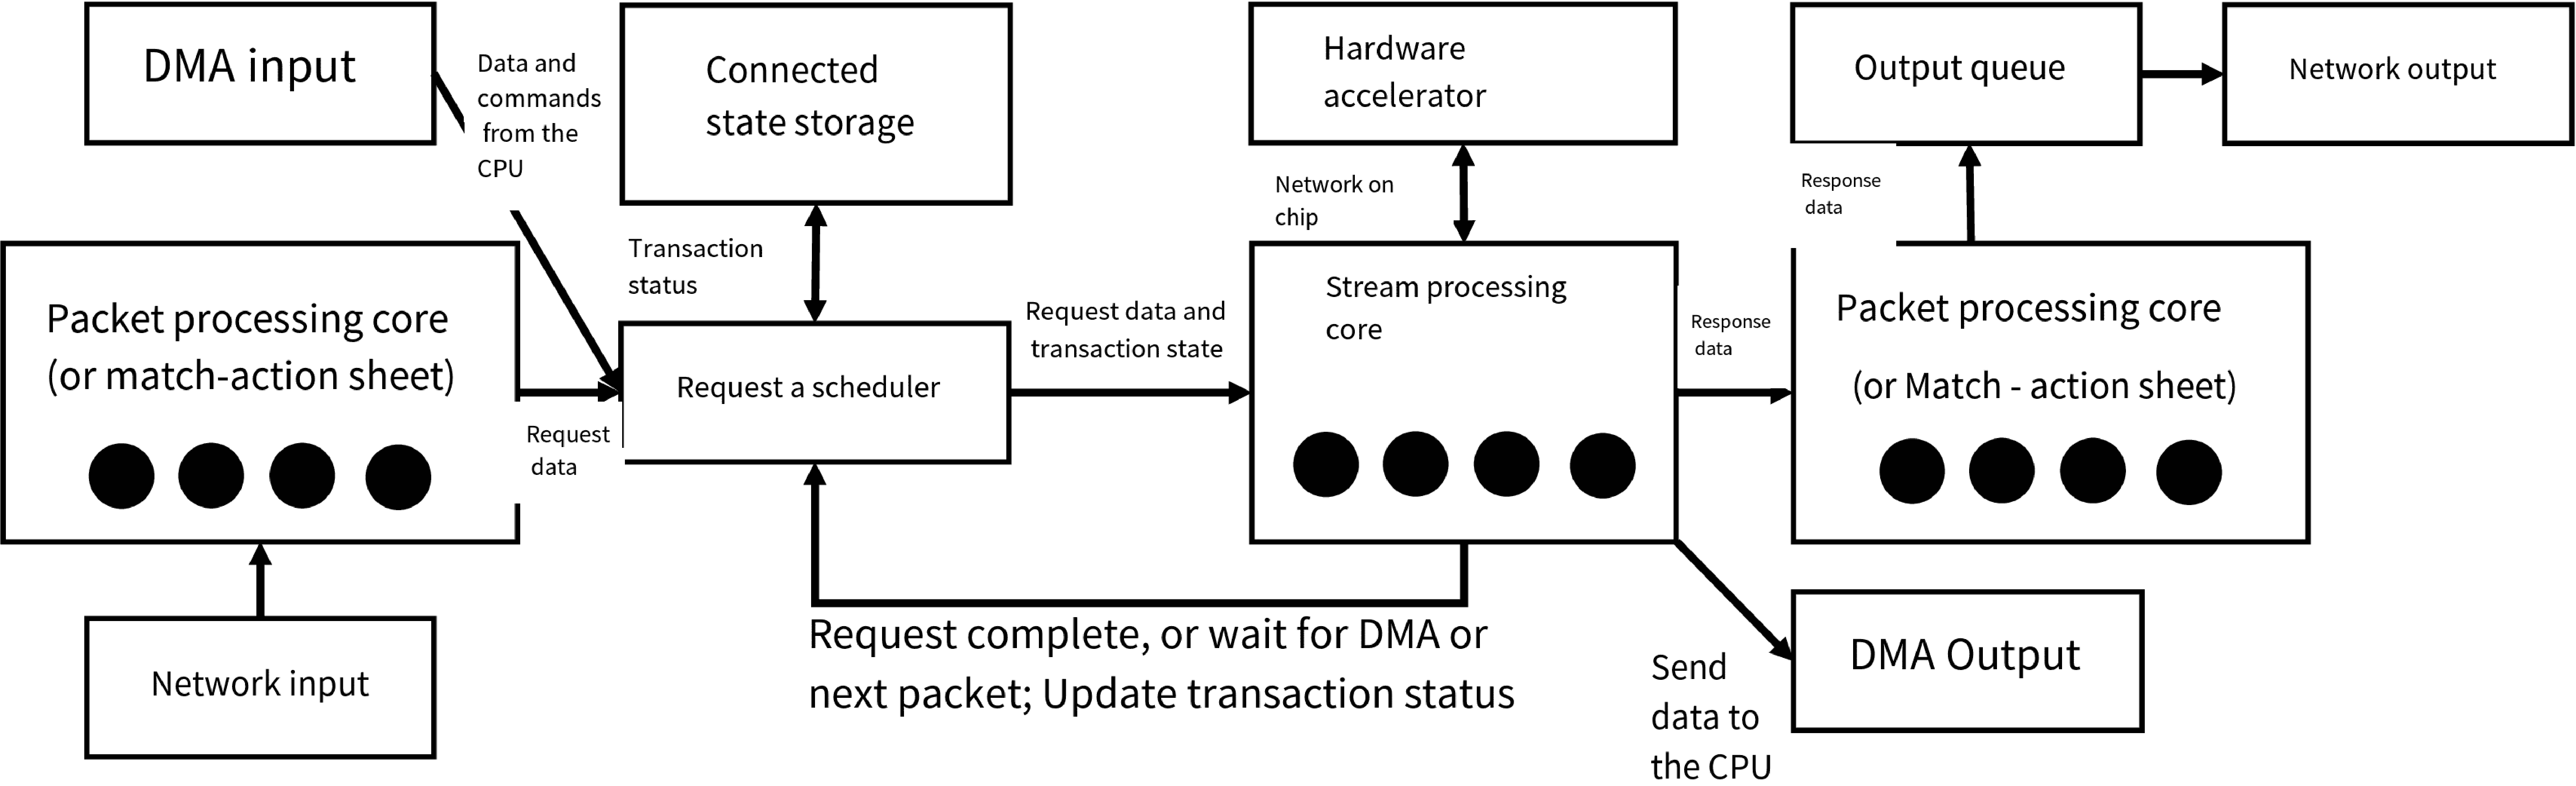
\includegraphics[width=1.0\textwidth]{figures/network_processor.pdf}
	\caption{网络处理器的一般架构。}
	\label{background:fig:network_processor}
\end{figure}


网络处理器之所以能比通用处理器更高效地处理网络数据包和主机请求,是因为它把很多数据包处理功能固化成了硬件逻辑。
第一,在保证服务质量(QoS)的调度器方面,硬件调度器可以实现是中心化先到先处理调度模型(c-FCFS),而网卡根据连接哈希来进行分派的 RSS 技术试图模拟分布式先到先处理调度模型(d-FCFS) \cite{kaffes2019shinjuku,ousterhout2019shenango}。中心化调度中,中心调度器维护一个调度队列,并将队首任务分派给刚刚处理完上一任务的处理器。分布式调度中,中心调度器将请求均匀分派到各个处理器的队列,每个处理器只能处理自己的队列,因此可能存在有的处理器队列非空而其他处理器闲置的情况。排队论表明,c-FCFS 比 d-FCFS 的各个核心的负载更加均衡,请求处理的平均延迟和尾延迟也更低。况且,网卡 RSS 技术往往并不能准确地模拟 d-FCFS 模型,因为数据包的处理可能是有状态的,很多情况下需要把相同的连接分配给相同的处理器核心,这时只有在连接数量很大、每条连接的数据包数量相同时,才能模拟 d-FCFS 模型;而现实中每条连接的数据包数量常常呈现长尾分布,此时处理器核心的负载就是不均衡的。理论分析 \cite{li2017kv} 表明,长尾分布下负载的不均衡程度与处理器核心的数量正相关。例如,对 64 个流处理核心的网络处理器,如果使用根据哈希分配连接的 d-FCFS 方式,长尾分布下负载最高的核心负载是平均核心负载的 6 倍。

第二,网络处理器的数据包解析、查找表、数据结构、定时器、DMA 引擎等很多常用模块是用硬件实现的。这些查找表和数据结构如果用软件实现,将消耗较多的指令数,影响数据面处理性能。例如,在软件中设置和触发一次定时器约需要 200 条指令,解析 TCP/IP 协议报文需要约 100 条指令 \cite{clark1989analysis}。从延迟上看,在 1 GHz 的网络处理器中,如果需要把数据包发送延迟控制在 1.5 $\mu$s 以内,假设 PCIe 延迟为 0.3 $\mu$s,网络数据链路层(MAC)延迟为 0.2 $\mu$s,每个数据包在可编程网卡内的处理是串行的,则软件处理每个数据包的指令数不能超过 1000 条。从吞吐量上看,如果需要支持 40 Gbps 网络下的 64 字节小包线速(line-rate)处理,每秒需要处理 60 M 个数据包,假设网络处理器有 64 个处理核心,每个核心每秒能执行 1 G 条指令,则每个处理核心平均每个数据包的指令数不能超过 1000 条。因此,节约数据包处理的指令数对延迟和吞吐量都很重要。网络处理器通过用硬件实现常用数据结构和算法,大大减轻了数据包处理器和流处理器的负担。这些硬件模块与处理核心之间通常使用片上网络互连,使得处理核心可以在处理过程中随时调用这些模块。

第三,网络处理器内流处理核心的线程调度与上下文管理是由硬件实现的,因此可以实现细粒度的延迟隐藏。例如,流处理核心如果调用了一个需要较长时间的 DMA 操作,或者需要等待一个定时器,硬件会自动保存其现场(包括寄存器和正在处理的流状态),将该线程放入未就绪队列,并切换到就绪队列中的下一线程;如果就绪队列为空,且并发线程数尚未达到硬件限制,则可以从任务队列中取出下一任务,新建一个线程。当 DMA 操作返回或定时器被触发时,未就绪队列中的线程就被切换到就绪队列。大多数网络处理器使用如上所述的非抢占式协作调度。为了支持严格优先级的服务质量保证,并在高优先级流量较小时能够充分利用处理能力来处理低优先级流量,一些网络处理器具备抢占式调度功能。不同于主机上的 CPU,网络处理器把操作系统的上下文管理和调度功能用硬件实现,相比 CPU 大大降低了上下文切换的开销。在数据中心场景下,CPU 应用程序的微秒级延迟隐藏成为越来越重要的问题 \cite{barroso2017attack},网络处理器的 ``硬件操作系统'' 设计也可以给主机 CPU 的设计带来一些启示。

第四,网络处理器内的内存层次结构是定制化的,因此访存的效率比通用处理器高,这点与 FPGA 的体系结构优势相似。通用处理器的 ``内存墙'' 问题是众所周知的,所有流处理核心如果都从共享内存中读写流状态,缓存一致性的开销是很高的,给处理器的设计带来了很多负担。而网络处理器在硬件中实现了数据包内容与数据包处理核心的绑定、流状态与流处理核心的绑定,数据包内容和流状态通过定制的数据通路进行搬运和缓存,在相同芯片面积和制程下,提高了内存带宽。

需要指出的是,虽然网络处理器相比通用处理器能耗效率更高,但编程较为困难。早期的网络处理器通常使用专用指令集的微码(microcode)进行编程,由于缺少编译器,编程语言的抽象程度与汇编相似。现代网络处理器一般使用通用 CPU 核心(如 ARM 和 MIPS)作为数据包处理器和流处理器,因而可以利用完善的编译器和开发工具链,使用 C 语言编程。可编程网卡内硬化的功能则使用库函数的形式进行调用,类似 Intel CPU 上的原子操作和向量操作。相比通用处理器,现代可编程网卡的编程困难性主要体现在开发者需要花时间了解这些专有库函数和网卡的体系结构,也不能直接使用通用处理器上成熟的基于 DPDK 等框架的代码。

在性能方面,网络处理器最大的问题是单核的性能较低,导致两个后果。
首先,有状态流往往只映射到一个处理核心或线程,以防止在单个流中进行状态分片和无序处理。即使一些网络处理器支持把有状态处理划分为多个阶段,并用多核流水线化处理,但流水级的数量受到硬件和流处理逻辑依赖的限制。
因此,对有状态处理而言,单流的数据包吞吐量不能超过网络处理器单核处理能力的数倍。
单核性能较低的第二个后果是为了支持更高的网络带宽,处理核心的数量必须线性增长,不仅增加了芯片面积和耗电量,也给核心间互连、内存层次、片上网络的设计带来了挑战。
在 40 Gbps 及以上的更高网络速度下,核心数量显著增加。分散和收集数据包的片上网络和调度程序变得越来越复杂和低效。将数据包送入处理核心,处理数据包,再发送到网络的整个流程经常需要 10 $\mu$s 或更多的延迟。
此时的延迟明显高于专用芯片,并且具有更大的可变性。


业界的网络处理器产品包括 Netronome NFP-32xx,Cavium OCTEON,Tilera,Mellanox NP-5 等。其中有些网络处理器只有流处理核心,没有数据包处理核心,但总体架构是类似的。




\subsection{通用处理器(SoC)}
\label{smartnic-soc}

注意到网络处理器较难编程的问题,业界提出了基于通用处理器的可编程网卡架构。
此架构与 2011 年微软亚洲研究院提出的 ServerSwitch~\cite{lu2011serverswitch} 架构类似,由一个硬件网络交换机和一个通用处理器构成。
例如,Mellanox BlueField \cite{mellanox-bluefield} 可编程网卡由一个 Mellanox ConnectX-5 硬件网卡和一个多核 ARM 处理器构成。
其中硬件网卡就是第 \ref{smartnic-asic} 节讨论的专用芯片。
如图 \ref{background:fig:smartnic_soc} 所示,多核 ARM 处理器、Mellanox ConnectX-5 网卡通过一个 PCIe 交换机互连。PCIe 交换机进一步连接到主机 CPU 上,实现多核处理器、硬件网卡(即网络交换机)和主机 CPU 之间三方的互连。
网络交换机实现了基本的数据包解析、分类、排队和转发功能,与第 \ref{smartnic-asic} 节所讨论的类似。
多核 ARM 处理器从硬件网卡接收数据包,进行处理后传递给主机 CPU,或者返回硬件网卡。


\begin{figure}[htbp]
	\centering
	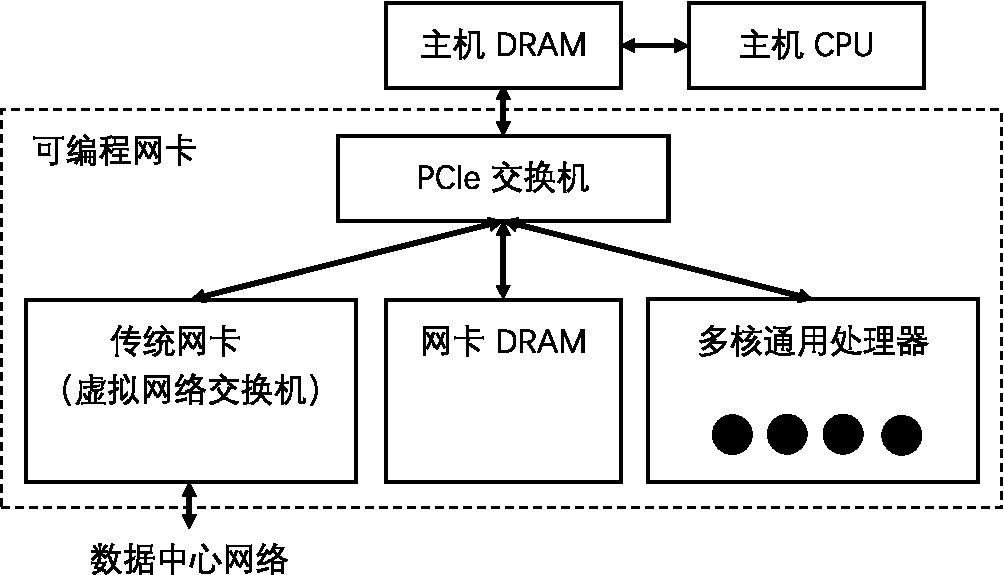
\includegraphics[width=0.6\textwidth]{figures/smartnic_soc.pdf}
	\caption{基于通用处理器的可编程网卡架构。}
	\label{background:fig:smartnic_soc}
\end{figure}

基于多核通用处理器的 SoC 架构与基于网络处理器的 NP 架构有很多相似之处,也因此经常被统称为同一类架构,但事实上它们有很多区别。表 \ref{background:tab:soc-vs-np} 比较了用于数据中心可编程网卡的 SoC 和 NP 架构。

\begin{table}[htbp]
	\centering
	\caption{多核通用处理器与网络处理器架构的比较。}
	\scalebox{0.9}{
	\begin{tabular}{l|p{.35\textwidth}|p{.35\textwidth}}
		\hline
		比较项目 & 多核通用处理器(SoC) & 网络处理器(NP) \\
		\hline
		\hline
		指令类型 & ARM / MIPS 标准指令集 & ARM / MIPS 扩展指令集 \\
		\hline
		操作系统 & 通用操作系统(如 Linux) & 无操作系统或定制化操作系统 \\
		\hline
		操作系统、分页等 & 支持 & 一般不支持 \\
		\hline
		内存结构 & 统一寻址 & 统一寻址和定制数据通路结合 \\
		\hline
		数据包处理框架 & 通用(如 DPDK) & 可编程网卡专用 \\
		\hline
		多核排队模型 & d-FCFS(硬件分派) & c-FCFS(硬件调度) \\
		\hline
		平均处理延迟 & 约 5 $\mu$s & 小于 2 $\mu$s \\
		\hline
		单核处理能力 & 约 3 M pps & 约 1 M pps \\
		\hline
		处理器核心数量 & 约 8 个 & 约 64 个 \\
		\hline
		总数据包处理能力 & 约 24 M pps & 约 64 M pps \\
		\hline
		功耗 & \multicolumn{2}{c}{10 W 至 20 W} \\ 
		\hline
	\end{tabular}
	}
	\label{background:tab:soc-vs-np}
\end{table}


表面上看,可编程网卡与服务器主机 CPU 都使用通用处理器,但如表 \ref{background:tab:host-cpu} 所示,无论在成本还是性能功耗方面,可编程网卡使用的通用处理器都有较明显的优势。此外,如第 \ref{chapter:intro} 章所讨论的,在云计算数据中心,主机 CPU 可以用于出售,其潜在售价远高于单一 CPU 组件的硬件价格。因此,在数据中心使用嵌入在可编程网卡内的通用处理器,比传统上使用主机 CPU 的方法仍然是有优势的。

\begin{table}[htbp]
	\centering
	\caption{可编程网卡内的通用处理器与主机 CPU 的比较。}
	\scalebox{0.9}{
	\begin{tabular}{l|p{.35\textwidth}|p{.35\textwidth}}
		\hline
		比较项目 & 可编程网卡通用处理器 & 服务器 CPU \\
		\hline
		\hline
		架构 & RISC(ARM / MIPS) & x86 \\
		\hline
		时钟频率 & 1 至 2 GHz & 2 至 3 GHz  \\
		\hline
		功耗 & 10 W 至 20 W & 约 100 W \\
		\hline
		价格 & 数十至上百美元 & 数百至上千美元 \\
		\hline
		单核处理能力 & 约 3 M pps & 约 5 M pps \\
		\hline
		处理器核心数量 & 约 8 个 & 约 20 个 \\
		\hline
		总数据包处理能力 & 约 24 M pps & 约 100 M pps \\
		\hline
		是否支持虚拟化 & 不一定 & 支持 \\
		\hline
		平均处理延迟 & \multicolumn{2}{c}{约 5 $\mu$s} \\
		\hline
		操作系统 & \multicolumn{2}{c}{通用操作系统(如 Linux)} \\
		\hline 
		数据包处理框架 & \multicolumn{2}{c}{通用(如 DPDK)} \\
		\hline
	\end{tabular}
	}
	\label{background:tab:host-cpu}
\end{table}


基于多核SoC的网卡使用大量的嵌入式CPU内核来处理数据包,交换一些性能以提供比ASIC设计更好的可编程性。相比网络处理器,多核 SoC 更容易编程,即可以采用标准的DPDK样式代码并在熟悉的Linux环境中运行。现有基于主机 CPU 的网络功能代码也很容易交叉编译到多核 SoC 上运行,而网络处理器的代码一般需要重新编写。

与前面网络处理器一节讨论的相同,多核 SoC 和网络处理器都受限于单核性能。
尽管多核 SoC 的单核性能高于网络处理器,但多核 SoC 的核间通信开销高于网络处理器处理核心组成的硬件流水线,从而多核 SoC 中每个数据包一般是在一个处理器核心上处理到完成(run-to-completion)。因此,单流性能一般是在同一数量级的,即在 5 M pps(数据包每秒)左右。
在核心数量增加方面,由于多核 SoC 大多采用分布式先到先服务调度(d-FCFS)模型,如果软件不使用核间工作窃取(work stealing)等技术,处理器间负载的不均衡会随核心数量的增加变得越来越严重。
在延迟方面,由于多核 SoC 处理器间的负载不平衡,以及多核 SoC 采用通用操作系统和通用的共享内存层次带来的操作系统调度、中断和缓存不命中等非确定性延迟,多核 SoC 的延迟稳定性一般比网络处理器更低,尾延迟(tail latency)一般比网络处理器更高。

因此,虽然多核 SoC 方法具有明显的优点,即具有熟悉的编程模型和良好的应用兼容性,但在更高的网络速度下,单流性能、更高的延迟和更差的可扩展性需要另一种解决方案。


\subsection{可重构硬件(FPGA)}
\label{smartnic-fpga}

众所周知,通用处理器(CPU)的摩尔定律已入暮年,而机器学习和 Web服务的规模却在指数级增长。人们使用定制硬件来加速常见的计算任务,然而日新月异的行业又要求这些定制的硬件可被重新编程来执行新类型的计算任务。FPGA (Field Programmable Gate Array) 是一种硬件可重构的体系结构,常年来被用作专用芯片(ASIC)的小批量替代品。近年来FPGA在数据中心大规模部署,以同时提供强大的计算能力和足够的灵活性。2016年,Intel公司以167亿美元的价格收购FPGA巨头Altera公司,以保持其在数据中心领域的领导地位,并探索CPU与FPGA结合的异构服务器计算架构。


FPGA(Field Programmable Gate Array,可编程门阵列)是一种可以重新定制(reconfigurable)的集成电路元器件。直观上来说,FPGA 就是一个可以用编程的方法重新组合的一大堆电子元器件。这些元器件包括逻辑门(如与,或,非门),寄存器 (Register),加法器,静态内存(SRAM)等等,用户可以定制它们之间的连接从而组成不同的电路。如今的FPGA除了基本元件,还加入了越来越多的DSP和硬核(hard IP),以提高乘法、浮点运算和访问外围设备的性能。FPGA的优点是技术比较成熟,开发门槛相对其它集成电路(如ASIC)较低,部署后依然可以修改,缺点是性能比专用芯片差。
图\ref{clicknp:fig:fpga}显示了FPGA板的逻辑图。


\begin{figure}[t]
	\centering
	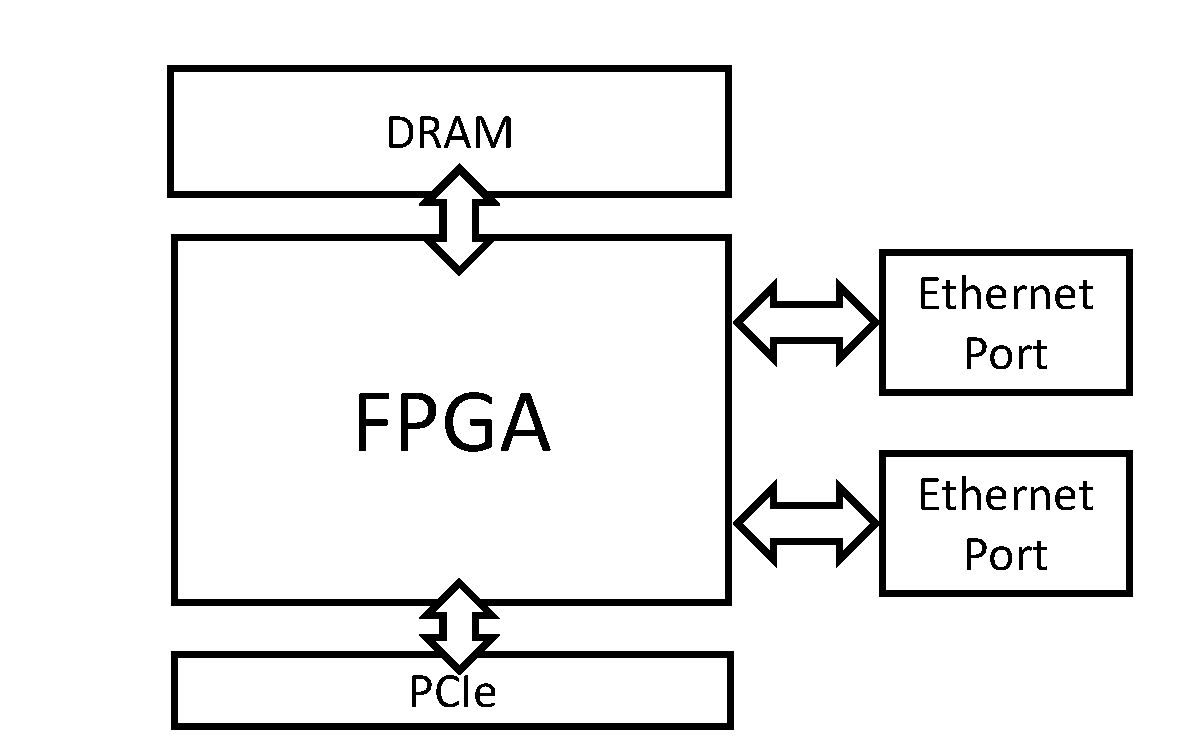
\includegraphics[width=0.6\textwidth]{fpga-board.pdf}
	
	\caption{FPGA板的逻辑图。}
	\label{clicknp:fig:fpga}
	
\end{figure}



以CPU为代表的通用处理器通常采用冯·诺依曼结构及其变体(下称冯氏结构)。冯氏结构中,由于执行单元(如 CPU核)可能执行任意指令,就需要有指令存储器、译码器、各种指令的运算器、分支跳转处理逻辑。由于指令流的控制逻辑复杂,不可能有太多条独立的指令流,因此GPU 使用 SIMD(单指令流多数据流)来让多个执行单元以同样的步调处理不同的数据,CPU 也支持 SIMD指令。而 FPGA 每个逻辑单元的功能在重编程(烧写)时就已经确定,不需要指令。

冯氏结构中使用内存有两种作用。一是保存状态,二是在执行单元间通信。由于内存是共享的,就需要做访问仲裁;为了利用访问局部性,每个执行单元有一个私有的缓存,这就要维持执行部件间缓存的一致性。对于保存状态的需求,FPGA 中的寄存器和片上内存(BRAM)是属于各自的控制逻辑的,无需不必要的仲裁和缓存。对于通信的需求,FPGA 每个逻辑单元与周围逻辑单元的连接在重编程(烧写)时就已经确定,并不需要通过共享内存来通信。

FPGA 实际的表现如何呢?下面分别讨论计算密集型任务和通信密集型任务。

计算密集型任务的例子包括矩阵运算、图像处理、机器学习、压缩、非对称加密、必应搜索的排序等。这类任务一般是 CPU把任务卸载(offload)给 FPGA 去执行。对这类任务,Intel Stratix V FPGA 的整数乘法运算性能与 20 核的 CPU 基本相当,浮点乘法运算性能与 8 核的 CPU 基本相当,而比 GPU 低一个数量级。下一代 FPGA,Stratix 10,将配备更多的乘法器和硬件浮点运算部件,从而理论上可达到与现在的顶级 GPU 计算卡旗鼓相当的计算能力。

在数据中心,FPGA 相比 GPU 的核心优势在于延迟。像 Bing 搜索排序这样的任务,要尽可能快地返回搜索结果,就需要尽可能降低每一步的延迟。如果使用 GPU 来加速,要想充分利用 GPU 的计算能力,batch size 就不能太小,延迟将高达毫秒量级。使用作为 PCIe 加速卡的 FPGA 来加速,则只需微秒级的 PCIe 延迟。未来 Intel 推出通过 QPI 连接的 Xeon + FPGA 之后,CPU 和 FPGA 之间的延迟更可以降到 100 纳秒以下,跟访问主存没什么区别了。

FPGA 为什么比 GPU 的延迟低这么多?这本质上是体系结构的区别。FPGA 同时拥有流水线并行和数据并行,而 GPU 几乎只有数据并行(流水线深度受限)。例如处理一个数据包有 10 个步骤,FPGA 可以搭建一个 10 级流水线,流水线的不同级在处理不同的数据包,每个数据包流经 10 级之后处理完成。每处理完成一个数据包,就能马上输出。而 GPU 的数据并行方法是做 10 个计算单元,每个计算单元也在处理不同的数据包,然而所有的计算单元必须按照统一的步调,做相同的事情(SIMD,Single Instruction Multiple Data)。这就要求 10 个数据包必须一起输入、一起输出,输入输出的延迟增加了。当任务是逐个而非成批到达的时候,流水线并行比数据并行可实现更低的延迟。因此对流式计算的任务,FPGA 比 GPU 天生有延迟方面的优势。

ASIC 专用芯片在吞吐量、延迟和功耗三方面都无可指摘,但微软并没有采用,主要出于两个原因:
第一,数据中心的计算任务是灵活多变的,而 ASIC研发成本高、周期长。例如,如果大规模部署了一批某种神经网络的加速卡,然而另一种神经网络变得更流行了,则投资的回报率将变得较低。FPGA只需要几百毫秒就可以更新逻辑功能。FPGA 的灵活性可以保护投资,事实上,微软目前的 FPGA 使用方法与最初的设想大不相同。
第二,数据中心是供不同的租户使用的,如果有的机器上有神经网络加速卡,有的机器上有必应搜索加速卡,有的机器上有网络虚拟化加速卡,任务的调度和服务器的运维会很麻烦。使用FPGA 可以保持数据中心的同构性。

接下来看通信密集型任务。相比计算密集型任务,通信密集型任务对每个输入数据的处理不甚复杂,基本上简单算算就输出了,这时通信往往会成为瓶颈。对称加密、防火墙、网络虚拟化都是通信密集型的例子。

对通信密集型任务,FPGA 相比 CPU、GPU 的优势就更大了。从吞吐量上讲,FPGA 上的收发器可以接入 40 Gbps 甚至 100 Gbps 的光纤,以线速处理任意大小的数据包;而 CPU需要从网卡把数据包收上来才能处理,很多网卡是不能线速处理 64 字节的小数据包的。尽管可以通过多块网卡来达到高性能,但CPU 和主板支持的 PCIe 插槽数量往往有限,而且网卡、交换机本身也价格不菲。

从延迟上讲,网卡把数据包收到 CPU,CPU 再发给网卡,即使使用 DPDK 这样高性能的数据包处理框架,延迟也有 4 至 5 微秒。更严重的问题是,通用 CPU 的延迟不够稳定。例如当负载较高时,转发延迟可能升到几十微秒甚至更高;现代操作系统中的时钟中断和任务调度也增加了延迟的不确定性。

虽然 GPU 也可以高性能处理数据包,但 GPU 是没有网口的,意味着需要首先把数据包由网卡收上来,再让 GPU 去做处理。这样吞吐量受到 CPU 和/或网卡的限制。GPU 本身的延迟就更不必说了。

综上,在数据中心里 FPGA 的主要优势是稳定又极低的延迟,适用于流式的计算密集型任务和通信密集型任务。

FPGA 也并不是万能药,主要有如下几方面的挑战。

第一,与CPU或GPU相比,FPGA通常具有更低的时钟频率和更小的存储器带宽。
例如,FPGA的典型时钟频率约为200MHz,比CPU慢一个数量级(2至3~GHz)。
同样,FPGA的单块存储器或外部DRAM的带宽通常为2至10~GBps,而内存带宽约为Intel XEON CPU的40~GBps,GPU为100~GBps。
但是,CPU或GPU只有有限的内核,这限制了并行性。 FPGA内置了大量的并行性。
现代FPGA可能拥有数百万个LE,数百个K位寄存器,数十个M位BRAM和数千个DSP模块。从理论上讲,它们中的每一个都可以并行工作。
因此,FPGA芯片内部可能会同时运行数千个并行的``\textit {核}''。
虽然单个BRAM的带宽可能有限,但如果并行访问数千个BRAM,则总内存带宽可以是多TBps!
因此,为了实现高性能,程序员必须充分利用这种大规模的并行性。

第二,传统上,FPGA使用诸如Verilog和VHDL之类的硬件描述语言(HDL)进行编程。
这些语言的抽象层次较低,难以学习,编程也很复杂。
尽管近年来 Chisel 等高层次硬件描述语言开始流行,但仍然需要程序员具有数字逻辑设计的基础知识和硬件设计的思维方式。
因此,大型软件程序员社区已经远离FPGA多年了~\cite {bacon2013fpga}。
为了简化这一点,许多高级综合(HLS)工具/系统已经在工业界和学术界开发,试图将高级语言(主要是C)的程序转换为HDL。
但是,正如第 \ref{chapter:clicknp} 章中将讨论的,它们或者没有充分利用 FPGA 中大规模的并行性,或者延迟过高,或者只是硬件开发工具链的补充,因而都不适合网络功能处理。这将是第 \ref{chapter:clicknp} 章的重点。

第三,与基于指令的处理器相比,FPGA 的任务切换开销较高。一方面,尽管 FPGA 可以通过动态重配置(dynamic reconfiguration)来实现数据面无中断的任务切换,但这样就必须固定一部分资源在 FPGA 芯片上的物理位置,使得 FPGA 放置(placement)和路由(routing)的全局优化受到限制;还需要增加逻辑来辅助动态重配置。这带来了 FPGA 面积的开销。
另一方面,FPGA 动态重配置需要几十毫秒的时间,远长于 CPU 任务切换的时间(基于通用操作系统的 CPU 任务切换一般为数微秒,基于专用操作系统的 CPU 任务切换一般为数百纳秒,基于专用处理器的任务切换可在数十纳秒内完成)。这使得 FPGA 不能像 CPU 那样实现细粒度的分时复用。因此,目前 FPGA 的多用户复用主要是在空间上而非时间上,类似把不同的 CPU 核心分配给不同的虚拟机。此外,FPGA 动态重配置期间,用户逻辑无法工作,因此需要 CPU 在这段时间内代替 FPGA 进行处理,或者暂停 FPGA 的服务,从而影响服务质量。
本文所讨论的 FPGA 可编程网卡均为数据中心基础架构的第一方(first party)用途,而不是对外公开出售的第三方(third party)用途,因此几乎没有动态切换任务的需求;主要的挑战是利用动态重配置实现服务升级,并在升级期间实现服务质量保证。本文作者参与(但非主导)的一项工作 Feniks \cite{zhang2017feniks} 和最近的 AmorphOS \cite{khawaja2018sharing} 旨在解决此问题。

第四,FPGA 能用数字电路的逻辑规模受到 FPGA 可重构单元数量的限制,而后者又受到芯片面积的限制。因此,FPGA 不适合用来实现非常复杂的逻辑。对于逻辑复杂的情况,一般需要区分控制面和数据面,在 FPGA 中实现数据面,并在通用处理器上实现控制面。这也是贯穿本文始终的设计思想。相比使用通用处理器的可编程网卡,使用 FPGA 就增加了分离控制面与数据面的编程复杂性。

第五,一些类型的工作负载是计算密集型的,且在 FPGA 内实现的效率明显低于专用芯片。
第一类是加密解密等标准化操作。例如,Intel QuickAssist 加速卡 \cite{intel-qat} 基于 ASIC 的 RSA 非对称加密比第 \ref{chapter:clicknp} 章基于 FPGA 的实现,吞吐量约高 10 倍。
第二类是查找表等常见数据结构。例如,内容寻址内存(Content-Addressable Memory,CAM)是很多并发操作调度器和数据结构的基础。CAM 在专用芯片中可以用三态门实现,而在 FPGA 中实现的效率较低。
第 \ref{future:progammable_nic} 节的未来工作展望将提出借鉴网络处理器的架构,将这些 FPGA 内实现效率不高的操作硬化。

\iffalse
\subsection{架构对比}
\label{smartnic-comparison}

性能逐渐降低,可编程性逐渐提高。

如何选择,考虑几个方面:
\fi

\section{可编程网卡在数据中心的应用}
\label{background:sec:application}

微软 Azure、亚马逊 AWS、阿里云、腾讯云、华为云等云服务商先后公开了基于可编程网卡的数据中心加速实践。

\subsection{微软 Azure 云}

微软 Azure 云是业界最早尝试大规模使用 FPGA 加速数据中心的云计算平台。

微软部署定制化硬件(FPGA)的用途主要包括计算和基础架构两大方面:

\begin{itemize}
	\item 计算加速:
	\begin{enumerate}
		\item 2013 年起,用于必应(Bing)搜索的文档选择和排序算法 \cite{putnam2014reconfigurable};2016 年起,使用硬件微服务(hardware microservice)将多个 FPGA 上没有占用完全的资源整合(consolidate)到较少数量的 FPGA 上,提高 FPGA 的使用率。
		\item 压缩和加密算法 \cite{a-scalable-high-bandwidth-architecture-for-lossless-compression-on-fpgas};早期仅用于必应搜索,后期扩展到 Office 365、Cosmos / Azure 数据湖(data lake)、Onedrive、云存储等服务。
		\item 2015 年起,用于机器学习推理 \cite{accelerating-deep-convolutional-neural-networks-using-specialized-hardware,toward-accelerating-deep-learning-scale-using-specialized-hardware-datacenter,serving-dnns-real-time-datacenter-scale-project-brainwave,a-configurable-cloud-scale-dnn-processor-for-real-time-ai};不仅支持深度学习模型,还支持传统机器学习模型。
		\item 2016 年起,推出 FPGA 实例的虚拟机,对第三方出租 FPGA 算力。
	\end{enumerate}
	\item 基础架构:
	\begin{enumerate}
		\item 网络:2015 年开始,用于网络虚拟化加速 \cite{smartnic}。
		\item 持久化存储:加速 Azure 云存储 \cite{calder2011windows},一方面是在存储后端节点上,利用计算加速部分的压缩和加密算法,提高吞吐量,采用更好(但计算量更大)的压缩算法提高压缩率,节约存储空间;另一方面是在存储前端节点和计算节点上的存储服务,通过 FPGA 加速存储协议栈的数据面,实现数据面绕过虚拟机监控器(hypervisor)并能按照服务质量保证共享存储资源。
	\end{enumerate}
\end{itemize}


考虑到上述需要加速的工作负载,微软在选择数据中心加速硬件时,主要从三个方面考虑 \cite{putnam2014reconfigurable}:

\begin{enumerate}
	\item CPU 和加速器间的通信方式:
	\begin{enumerate}
		\item 一致性内存(coherent memory),虽然编程简单,但在 PCIe 总线上不容易实现高效率;
		\item 直接内存访问(DMA),作为 PCIe 总线上标准的通信模式,这是微软 FPGA 选定的方式。
		\item 网络,带宽和延迟较为受限。
	\end{enumerate}
	\item 加速器之间的连接范围:
	\begin{enumerate}
		\item 单机,性能不可扩放;
		\item 机架,使用定制互连,带宽可以较高,但添加定制互连的成本较高;
		\item 数据中心,使用数据中心现有的网络和交换机,成本较低,带宽和延迟也可以满足大多数应用的需求。
	\end{enumerate}
	\item 加速设备:
	\begin{enumerate}
		\item FPGA,同时适用于计算密集型与通信密集型负载,且具有低延迟,大规模部署情况下单位算力的成本较低,但编程复杂性高;
		\item GPU,适用于计算密集型负载的加速设备,比 FPGA 编程简单,但延迟较高;即使大规模部署,单位算力的成本仍然较高;
		\item 专用芯片 ASIC,同时适用于计算密集型与通信密集型负载,延迟最低,单位功耗的算力最高,但功能固化后的灵活性较差。例如上述工作负载从必应搜索扩展到压缩加密、网络、存储、机器学习、深度学习等,是一个逐步发展的过程,专用芯片的设计很难一步到位,而重新设计一款专用芯片需要一到两年的时间和数千万美元的一次性研发成本(NRE)。
	\end{enumerate}
\end{enumerate}





微软对于把 FPGA 部署在哪里这个问题,大致经历了三个阶段 \cite{configurable-cloud-acceleration}:
\begin{enumerate}
	\item 专用的 FPGA 集群,里面插满了 FPGA;
	\item 每台机器一块 FPGA,采用专用网络连接;
	\item 每台机器一块 FPGA,位于网卡和交换机之间,共享服务器网络。
\end{enumerate}

第一个阶段是专用集群,里面插满了 FPGA 加速卡,就像是一个 FPGA 组成的超级计算机。像超级计算机一样的部署方式有几个问题:

\begin{enumerate}
	\item 不同机器的 FPGA 之间无法通信,FPGA 所能处理问题的规模受限于单台服务器上 FPGA 的数量;
	\item 数据中心里的其他机器要把任务集中发到这个加速机柜,构成了 in-cast 的网络流量特征,网络延迟很难做到稳定;
	\item FPGA 专用机柜构成了单点故障;
	\item 装 FPGA 的服务器是定制的,散热设计和运维都增加了复杂性。
\end{enumerate}

一种不那么激进的方式是,在每个机柜一面部署一台装满 FPGA 的服务器。这避免了上述问题 (2)(3),但(1)(4) 仍然没有解决。

第二个阶段,为了保证数据中心中服务器的同构性(这也是不用 ASIC 的一个重要原因),在每台服务器上插一块FPGA,FPGA 之间通过专用网络连接。这也是微软在 ISCA’14 上所发表论文采用的部署方式。

FPGA 采用Stratix V D5,有172K个ALM,2014个M20K片上内存,1590个 DSP。板上有一个8GB DDR3-1333 内存,一个PCIe Gen3 x8接口,两个10 Gbps网络接口。一个机柜之间的FPGA采用专用网络连接,一组10G网口8个一组连成环,另一组10G网口6个一组连成环,不使用交换机。

这样一个 1632 台服务器、1632 块 FPGA 的集群,把必应的搜索结果排序整体性能提高到了 2倍(换言之,节省了一半的服务器)。本地和远程的 FPGA 均可以降低搜索延迟,远程 FPGA的通信延迟相比搜索延迟可忽略。

FPGA 在必应的部署取得了成功,Catapult 项目继续在公司内扩张。微软内部拥有最多服务器的,就是云计算 Azure 部门了。Azure 部门急需解决的问题是网络和存储虚拟化带来的开销。Azure把虚拟机卖给客户,需要给虚拟机的网络提供防火墙、负载均衡、隧道、NAT等网络功能。由于云存储的物理存储跟计算节点是分离的,需要把数据从存储节点通过网络搬运过来,还要进行压缩和加密。

为了加速网络功能和存储虚拟化,微软把 FPGA 部署在网卡和交换机之间。一块 FPGA(加上板上内存和网络接口等)的功耗大约是30 W,仅增加了整个服务器功耗的十分之一。只要规模足够大,对FPGA价格过高的担心将是不必要的。每个 FPGA 有一个 4GB DDR3-1333 DRAM,通过两个 PCIe Gen3 x8 接口连接到一个 CPU socket(物理上是 PCIe Gen3 x16 接口,因为 FPGA 没有 PCIe Gen3 x16 的硬核(hard IP),就拆分为两个 PCIe Gen3 x8 接口使用)。微软SmartNIC可编程网卡的架构如图 \ref{background:fig:azure_fpga} 所示,其中FPGA位于网络和传统网卡之间。

\begin{figure}[htbp]
	\centering
	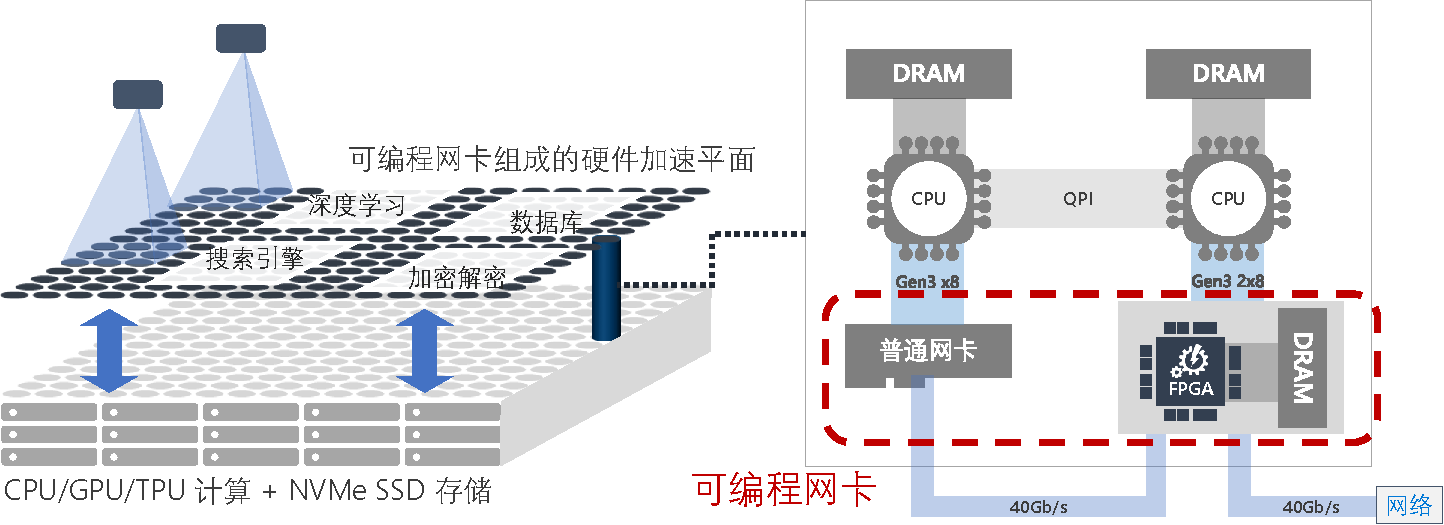
\includegraphics[width=0.8\textwidth]{figures/azure_fpga.pdf}
	\caption{微软基于 FPGA 的可编程网卡。}
	\label{background:fig:azure_fpga}
\end{figure}


FPGA(SmartNIC)对每个虚拟机虚拟出一块网卡,虚拟机通过 SR-IOV直接访问这块虚拟网卡。原本在虚拟交换机里面的数据平面功能被移到了 FPGA 里面,虚拟机收发网络数据包均不需要 CPU参与,也不需要经过物理网卡(NIC)。这样不仅节约了可用于出售的 CPU 资源,还提高了虚拟机的网络性能(25 Gbps),把同数据中心虚拟机之间的网络延迟降低了 10 倍 \cite{smartnic}。

这就是微软部署 FPGA 的第三代架构,也是目前 ``每台服务器一块 FPGA'' 大规模部署所采用的架构。FPGA 复用主机网络的初心是加速网络和存储,更深远的影响则是把 FPGA 之间的网络连接扩展到了整个数据中心的规模,做成真正云规模(cloud-scale)的 ``超级计算机'' \cite{configurable-cloud-acceleration}。第二代架构里面,FPGA 之间的网络连接局限于同一个机架以内,FPGA之间专网互连的方式很难扩大规模,通过 CPU 来转发则开销太高。

第三代架构中,FPGA 之间通过轻量级流控协议(Lightweight Transport Layer,LTL)通信。同一机架内延迟在 3微秒以内;8 微秒以内可达 1000 块 FPGA;20 微秒可达同一数据中心的所有 FPGA。第二代架构尽管 8台机器以内的延迟更低,但只能通过网络访问 48 块 FPGA。为了支持大范围的 FPGA 间通信,第三代架构中的 LTL 还支持PFC 流控协议和 DCQCN 拥塞控制协议。

通过高带宽、低延迟的网络互连的 FPGA构成了介于网络交换层和传统服务器软件之间的数据中心加速平面。除了每台提供云服务的服务器都需要的网络和存储虚拟化加速,FPGA上的剩余资源还可以用来加速必应搜索、深度神经网络(DNN)等计算任务。

对很多类型的应用,随着分布式 FPGA 加速器的规模扩大,其性能提升是超线性的。例如 CNN inference,当只用一块 FPGA 的时候,由于片上内存不足以放下整个模型,需要不断访问 DRAM 中的模型权重,性能瓶颈在DRAM;如果 FPGA 的数量足够多,每块 FPGA 负责模型中的一层或者一层中的若干个特征,使得模型权重完全载入片上内存,就消除了DRAM 的性能瓶颈,完全发挥出 FPGA 计算单元的性能。当然,拆得过细也会导致通信开销的增加。把任务拆分到分布式 FPGA集群的关键在于平衡计算和通信。


2016 年 9 月,《连线》(Wired)杂志发表了一篇《微软把未来押注在 FPGA 上》的报道 \cite{microsoft-wired-fpga},讲述了 Catapult 项目的前世今生。紧接着,Catapult 项目的负责人 Doug Burger 在 Ignite 2016 大会上与微软 CEO Satya Nadella 一起做了 FPGA 加速机器翻译的演示。演示的总计算能力是 103 万 T ops,也就是 1.03 Exa-op,相当于 10 万块顶级 GPU 计算卡。

在 MICRO'16 会议上,微软提出了硬件即服务(Hardware as a Service,HaaS)的概念 \cite{configurable-cloud-acceleration},即把硬件作为一种可调度的云服务,使得 FPGA 服务的集中调度、管理和大规模部署成为可能。通过硬件微服务,可以把原本运行在多个 FPGA 上的加速服务集中到少量的 FPGA 上,从而节约一定数量的 FPGA 运行其他类型的工作负载。

在 NSDI'18 会议上,微软发表了自 2015 年起将基于 FPGA 的可编程网卡用于网络虚拟化加速的实践 \cite{smartnic}。利用可编程网卡,Azure 虚拟机之间的吞吐量可高达 31 Gbps。同期,谷歌云平台(Google Cloud Platform,GCP)基于主机 CPU 软件的网络虚拟化实现 \cite{andromeda} 只能达到 16 Gbps 的吞吐量。亚马逊 AWS 基于通用处理器的 Nitro 网络虚拟化加速 \cite{nitro-talk} 只能达到 23 Gbps 的吞吐量。由于通用处理器单核性能的限制,AWS 的单个 TCP 流吞吐量只能达到 10 Gbps,而微软 Azure 和谷歌云平台的单流吞吐量均可达到虚拟机的峰值。这与本文第 \ref{smartnic-architecture} 节关于可编程网卡架构的讨论相符。

在延迟方面,使用 Linux 操作系统 TCP/IP 协议栈,微软 Azure 达到了 10 $\mu$s 的平均虚拟机间延迟,而使用内核绕过的 DPDK \cite{dpdk} 可以达到 5 $\mu$s 的平均延迟。同期,谷歌云平台的平均延迟为 20 $\mu$s,亚马逊 AWS 的平均延迟为 28 $\mu$s。使用 FPGA 加速后,微软 Azure 的尾延迟比平均延迟优势更加明显。例如,在 99.9\% 分位,Azure 的延迟为 20 $\mu$s,谷歌云平台基于主机 CPU 的延迟为 75 $\mu$s,亚马逊 AWS 基于可编程网卡通用处理器的延迟为 32 $\mu$s。在 99.99\% 分位,Azure 的延迟为 25 $\mu$s,而谷歌云平台和亚马逊 AWS 均达到或接近 100 $\mu$s。这是由于硬件流水线比软件处理的延迟更加可控,而软件处理中,由于主机 CPU 上运行着客户虚拟机,延迟不稳定性比可编程网卡上的通用处理器更高。



\subsection{亚马逊 AWS 云}

在 2017 年 12 月的 Re:Invent 大会上,亚马逊 AWS 云发布了名为 ``Nitro'' 的计算加速架构 \cite{nitro-blog}。
根据 2017 年 Re:Invent 大会和 2018 年 AWS 峰会上亚马逊发布的信息 \cite{nitro-talk,nitro-web},AWS 使用了定制 ASIC 来实现多种加速和安全功能。
最初,AWS 在 FPGA 和 ASIC 架构之间权衡,并决定采用 ASIC 方案。
为此,2015 年 1 月,亚马逊用 30 多亿美元收购了 ASIC 设计公司 Annapurna 实验室 \cite{annapurna},该公司以设计基于 ARM 核的片上系统(SoC)见长。

Nitro 项目的发展是分阶段的。与微软 Azure 类似,虚拟机的 I/O 瓶颈最早体现在虚拟网络上。早在 2013 年 11 月,AWS 的 C3 实例就引入了一块独立的网卡以实现高性能网络(enhanced networking),采用 SR-IOV 方式让虚拟机直接访问网卡,绕过虚拟机监控器中的虚拟交换机软件。此技术帮助 Netflix 实现了每秒 200 万个数据包的虚拟机网络吞吐量 \cite{netflix-aws}。

2015 年 1 月,AWS 的 C4 实例开始使用硬件加速弹性块存储(Elastic Block Storage,EBS)。弹性块存储的数据储存在存储节点上,而客户虚拟机运行在计算节点上,因此这是一种远程存储。对客户虚拟机而言,是一块虚拟存储设备,它是由虚拟机监控器 Xen Dom0 中的存储管理软件实现虚拟化的。C4 实例使用高性能网卡而非传统网卡来连接远程的弹性块存储,从而提高了性能。

2017 年 2 月,AWS 的 I3 实例引入了 NVMe 本地存储和专用的存储虚拟化芯片。以往,客户虚拟机访问本地存储,也需要经过虚拟机监控器中的存储管理软件,这是由于一台物理服务器中可能有多台虚拟机,每台虚拟机只能访问属于自己的那一部分存储空间,因此需要隔离。对延迟和吞吐量都很高的 NVMe 存储而言,存储虚拟化软件带来的开销太高了。为此,I3 实例引入的 Nitro 芯片在硬件上实现了存储隔离,因此可以通过 SR-IOV 把 NVMe 存储直通客户虚拟机,实现了每秒 300 万次 I/O 操作的存储性能 \cite{aws-local-storage}。

2017 年 11 月,AWS 的 C5 实例大幅改变了计算节点虚拟化的架构。首先,C4 实例中的远程存储仍然需要软件实现虚拟化,这一部分也可以像 I3 本地存储一样用硬件实现,不过块存储比本地存储的接口更复杂,因此硬件实现的难度更大。其次,在网络、远程和本地存储都已经使用硬件虚拟化后,事实上虚拟机监控器中的管理软件就只剩下数据平面的中断(APIC)功能和控制平面的管理功能了。控制平面的管理功能较为复杂,用纯数字逻辑显然是不现实的。为了把虚拟网络(VPC)、弹性块存储和虚拟化控制平面全部卸载(offload)到加速卡上,Nitro ASIC 采用了基于 ARM 核的片上系统架构,从而保持了数据平面的可编程性和灵活性,还能把控制平面一并卸载到加速卡上。

采用 Nitro 加速卡后,AWS 重新设计了一个轻量级的虚拟机监控器 Nitro 来取代 Xen,而原来运行在 Xen Dom0 上的控制平面转移到了 Nitro ASIC 里,客户虚拟机可以得到接近裸金属(bare-metal)主机的性能。此后,AWS 发布了裸金属实例,客户代码直接在物理机上运行,而所有的存储和网络资源都由 Nitro 卡提供。

Nitro 系列芯片主要包括三种芯片 \cite{nitro-blog,nitro-talk,nitro-web}:
\begin{enumerate}
	\item 云网络(VPC)和弹性块存储(EBS)加速芯片,一边连接数据中心网络,一边以 PCIe 卡的形式连接 CPU;
	\item 本地 NVMe 存储虚拟化芯片,作为 CPU 和 NVMe 存储设备之间的代理;
	\item 安全芯片,用于验证服务器中各种设备固件的版本,以及在裸金属服务器切换租户时重刷固件清除痕迹。
\end{enumerate}

Nitro 芯片的作用可以分为降低成本、提高性能和提高安全性三方面。下面详细讨论。

\textbf{节约 CPU 核。}
网络和存储虚拟化需要占用大量的 CPU 资源来处理每个网络包和存储 I/O 请求。
根据 ClickNP \cite{li2016clicknp} 估计,每个客户虚拟机的 CPU 核,需要预留另外 0.2 个 CPU 核来实现虚拟化。
如果这些功能可以被卸载到专用硬件,所节省的 CPU 核就可以用来安装客户虚拟机。
不管是考虑公有云虚拟机上每个 CPU 核的售价,还是考虑 Xeon CPU 每个核的硬件成本,用专用硬件都能获得明显的成本节约 \cite{smartnic}。

\textbf{提高最大核数。}
节约 CPU 核不仅能够降低成本,还能够提高大型虚拟机实例的最大核数。因为各大公有云厂商都从 Intel 等相同的厂商购买 CPU,因此同一时期能买到的最大 CPU 核数是相对固定的。虚拟化被卸载到硬件后,所有 CPU 核都用于运行客户虚拟机,因此 AWS 的 M5 实例最多可达 96 个 CPU 核。如果不使用硬件卸载,将只有 80 个 CPU 核可用于客户虚拟机,从而降低对追求极致性能客户的吸引力。

\textbf{提高单核频率。}
由于功耗墙的限制,CPU 的核心数目与平均核心频率不可兼得。同一代 CPU 架构下,较高核心频率的 CPU 核数一般较少。对于核数相等的虚拟机实例,如果使用传统的软件虚拟化,物理机就需要 1.2 倍的 CPU 核数,从而平均核心频率就可能降低。例如,在 C5 实例推出前的 72 核 EC2 实例,CPU 基频为 2.7 GHz,但采用同一代 Skylake 架构的 C5 实例虚拟机,CPU 基频就可以达到 3.0 GHz。

\textbf{提高本地存储性能。}
首先,在裸金属服务器上,本地 NVMe 存储可以达到每盘高达 400 K IOPS(I/O 操作每秒)的吞吐量。AWS I3 实例有 8 块 NVMe SSD,达到 3 M IOPS 的吞吐量。而对于常见的存储虚拟化协议栈,每个 CPU 核只能处理 100 K IOPS 左右的吞吐量,这意味着要占用 30 个 CPU 核才能让虚拟机充分利用 NVMe 存储的吞吐量,这个开销太高了。即使只有一块 NVMe 存储,4 个 CPU 核之间的负载均衡仍然是个难题 \cite{li2017kv}。如第 \ref{smartnic-architecture} 节所讨论的,由于硬件分配和处理任务是流水线式而非多个处理单元简单并行,硬件能够比多核软件更好地保证服务质量(QoS)。

其次,在延迟方面,裸金属服务器的 NVMe 存储平均延迟约为 80 微秒。虚拟化软件不仅会增加 20 微秒的平均延迟,而且由于操作系统调度、中断、缓存不命中等因素的影响,在高负载下的尾延迟(tail latency)可高达 1 毫秒(1000 微秒)。采用硬件卸载可以降低平均延迟 20\%,并降低高负载下的尾延迟 90\% 以上。

\textbf{提高远程存储性能和安全性。}
与本地存储类似,硬件加速可以提高远程存储性能。还有一点额外的优势:远程存储被公有云的所有租户共享,对可靠性和安全性要求更高。传统上远程存储协议在虚拟机监控器中运行,虽然逻辑上与客户虚拟机隔离,但由于共享 CPU、内存等资源,仍然不能排除零日(0-day)漏洞和边信道攻击的潜在安全隐患。把远程存储协议从主机 CPU 卸载到 Nitro 卡后,就有了更高的隔离性和更小的攻击表面(attack surface)。

\textbf{提高网络性能和安全性。}
在 Nitro 卡上实现网络虚拟化后,虚拟机可以直接通过 SR-IOV 访问网卡,达到数据中心网络 25 Gbps 的理论上限,尤其是对小数据包应用场景的性能提升明显。根据 ClickNP \cite{li2016clicknp} 估计,对 25 Gbps 线速(line-rate)的 64 字节小数据包,每秒高达 37 百万个,如果用软件虚拟交换机处理,将需要 60 个 CPU 核,这显然是不可接受的。因此大多数云服务商对虚拟网络(VPC)对吞吐量不仅有字节数的限制,还有数据包数的限制。大多数公有云的虚拟网络只支持数百万数据包每秒的吞吐量,需要处理大量小请求的远程过程调用(RPC)、键值存储(KVS)服务器就会遇到性能瓶颈。在延迟方面,软件虚拟化的 AWS 端到端延迟可达 100 微秒以上,而使用 Nitro 虚拟化加速后延迟就降低到 50 微秒以内了。硬件虚拟化对虚拟网络的尾延迟、服务质量和安全性的提升,也与远程存储相似。

\textbf{提高裸金属服务器安全性。}
最后,裸金属服务器上的客户代码可以直接访问服务器内的各种硬件设备,甚至可能烧写带外服务器管理(BMC)等组件的固件 \cite{bare-metal-security}。如果固件内被嵌入了恶意代码,并在下一个租户使用该裸金属服务器时被激活,后果不堪设想。事实上很大一部分客户选择裸金属服务器,正是出于对虚拟机隔离性的担忧。为了在租户开始使用裸金属服务器时提供安全和一致的硬件环境,Nitro 安全芯片会对固件进行重烧写。Nitro 还会在系统启动时进行完整性检查,这类似 UEFI 可信启动技术,但验证的范围不仅包括操作系统引导器,还包括硬件固件。

\subsection{阿里云、腾讯云、华为云、百度}

2018 年,我国云计算服务商也积极地在数据中心部署了可编程网卡。阿里云和腾讯云部署可编程网卡的首要目的是支持裸金属(bare-metal)服务器。相比虚拟机,裸金属服务器可以消除虚拟化带来的开销,实现同样硬件条件下最高的性能;方便部署客户自己的虚拟化软件(如 VMWare);与客户在自有数据中心(on-premises)的部署环境完全相同,降低客户上云的迁移开销;方便使用不支持虚拟化或虚拟化后性能有较大损失的硬件,如 GPU 和 RDMA 网卡;不与其他租户共享服务器硬件,隔离性和安全性更强,也能符合一些客户的合规要求。

在公有云中使用裸金属服务器的主要技术挑战是访问数据中心内的虚拟网络(VPC)和远程存储(EBS)等资源。一种简单的方法是在同一个机架(rack)内放置若干虚拟网络和存储服务器,部署相应的软件;并在柜顶交换机(ToR switch)上配置转发规则,使裸金属服务器的所有网络数据包经过虚拟网络和存储服务器。这种方法需要增加额外的服务器资源,提高了成本。另一种方法是把虚拟网络和存储的数据平面卸载到柜顶交换机上。但是,柜顶交换机的编程灵活性一般较差 \cite{tencent-smartnic},不足以支持虚拟存储的应用层协议和虚拟网络的安全规则等。

因此,在服务器上增加一块可编程网卡便成为支持裸金属服务器性能最高的方案。阿里和腾讯采用了 FPGA 数据平面与多核 CPU 控制平面结合的 SoC 方案。2018 年,阿里云发布的 ``神龙'' 裸金属服务器使用自研的 MOC 卡 \cite{alicloud-smartnic,alicloud-xdragon} 实现类似 AWS Nitro 的网络、存储虚拟化。腾讯云在 APNet’18 上发布了基于 FPGA 的可编程网卡方案,主要用于网络虚拟化 \cite{tencent-smartnic}。腾讯仅用 10 个硬件工程师,就在三个月内完成了 FPGA 逻辑设计,用四个月做出了可编程网卡的板卡,并在一年内部署 \cite{tencent-smartnic}。这是 FPGA 编程也可以实现敏捷开发的例证。腾讯正在把可编程网卡的应用范围从裸金属服务器扩展到普通虚拟机,并对两种应用场景使用统一的可编程网卡架构。

华为基于海思半导体的技术积累,发布了两款可编程网卡,同时也用于华为云虚拟网络的加速。SD100 系列可编程网卡 \cite{sd100} 采用了基于多核 ARM64 CPU 的 SoC 架构,数据平面和控制平面都运行在 ARM CPU 上。IN5500 系列可编程网卡 \cite{in200} 采用网络处理器(NP)提供数据平面的可编程性,可达到 100 Gbps 性能。利用可编程网卡,华为云发布了 C3ne 网络增强虚拟机实例,在国内云厂商中率先实现了每秒千万级的数据包转发 \cite{huawei-smartnic}。

百度虽然尚未发布可编程网卡加速的虚拟机实例,但在 FPGA 加速数据中心计算密集型应用方面是先行者。
早在 2010 年,百度就将 FPGA 用于数据压缩 \cite{ouyang2010fpga}。
2014 年,百度发布了将 FPGA 用于深度学习推理的 SDA 框架 \cite{ouyang2014sda},随后将 FPGA 用于数据库 SQL 处理 \cite{baidu-fpga-sql}。
2017 年,百度提出了基于 FPGA 的数据中心全栈加速器 XPU,将 FPGA 用于各种计算加速场景 \cite{ouyang2017xpu}。